\documentclass{subfile}


\begin{document}
	
	\section{Definitions and Propositions}
	Let us start from the very basics. Whenever you encounter a definition, try to make sense of it with examples. Try to get used to these terms and divisibility notation. It will not only make your life a lot easier, but also keep your solutions or ideas concise. So try not to get bored with the definitions\watermark.
	\begin{definition}\label{def:remainder}
		When an integer $a$ is divided by another integer $b$, we can write $a=bq+r$ for some integers $q$ and $r$. In this general case, we call $r$ the \textit{remainder} of the division.
		
		However, if we choose $q$ such that $0\leq r< |b|$, then we say $r$ is the \textit{minimum remainder} of the division\footnote{$|x|$ is the absolute value of $x$.}.
		
		At times, it is convenient to carry out the division so that $b$ is as close as possible to an integral multiple of $a$. Then we can write $a = bq + r$, with $|r| \leq |\frac{b}{2}|$ for some integer $q$.  In this case, we call $r$ the \textit{minimum absolute remainder}.  
	\end{definition}
	
	\begin{note}[1]
		We will prove later that the minimum remainder is unique. That is, there exists exactly one value for $r$ such that $a=bq+r$ and $0 \leq r <b$. Because of its uniqueness and positivity, remainder in this book will mean minimum remainder unless stated otherwise.
	\end{note}
	
	\begin{note}[2]
		When we talk about the the minimum absolute remainder in the division $a=bq+r$, note that if $b$ is odd, we will have a unique $r$. That is, there exist only one possible value for $r$ such that $|r| \leq |\frac{b}{2}|$. However, if $b$ and $a$ both are even, there can be two possible values for $r$. For example, if $b=20$ and $a=8$, the division can be done as both $20=8\cdot2+4$ and $20=3\cdot8-4$ and we would have two values for $r$: $4$ and $-4$. To force $r$ to be unique in this case, we will take the positive value of $r$ as the minimum absolute remainder. Therefore, in our example, $20=2\cdot8+4$ would be accepted as the division equation and $r=4$ is the minimum absolute remainder.
	\end{note}

In the next definition, we have swapped $a$ and $b$ and written $b=aq+r$ instead of $a=bq+r$. So, read carefully.
	
	\begin{definition}
		If $b=aq+r$ is the proper division of $b$ by $a$ (that is, a division in which $r$ is the minimum remainder), $b$ is the \textit{dividend}, $a$ is the \textit{divisor}, and $q$ is the \textit{quotient}.
	\end{definition}
	
	\begin{example}
		Let $b=23$ and $a=5$. The division of $b$ by $a$ can be done in many ways. Take $23=5\cdot2+13$, so we can say $13$ is a remainder of $23$ upon division by $5$, but not a minimum remainder. If we write the division as $23=5\cdot4+3$, then $3$ is the minimum remainder. And if we write it as $23=5\cdot5+(-2)$, then $-2$ is the minimum absolute remainder.
	\end{example}
	
	If we divide $4$ by $2$, we get a zero remainder. In this case, we say that $4$ is \textit{divisible} by $2$ and write it as $2\mid 4$.
	
	\begin{definition}
		Let $a$ and $b$ be two integers. If $b$ leaves a zero remainder upon division by $a$, or equivalently, if there is an integer $k$ for which $b=ak$, we write $a \mid b$ and say that
		\begin{itemize}
			\item $b$ is \textit{divisible} by $a$,
			\item $a$ \textit{divides} $b$,
			\item $a$ is a \textit{divisor} (or a \textit{factor}) of $b$, or
			\item $b$ is a \textit{multiple} of $a$.
		\end{itemize} 
		Likewise, $a\nmid b$ denotes that $b$ is not divisible by $a$. 
	\end{definition}
	
	\begin{remark}
		In some countries, authors use the notation $b\vdots a$ instead of $a|b$, but it is not as common.
	\end{remark}
	
	\begin{definition}
		If $a$ divides $b$ and $|a|<|b|$, the number $a$ is called a \textit{proper divisor} of $b$. Here, $|a|$ denotes the absolute value of $a$. For example, $|-5|=5$ and $|5|=5$.
	\end{definition}
	
	\begin{example}
		$4 \mid 20$ and $5 \mid 20$ but $11\nmid 20$.
	\end{example}
	
	\begin{example}
		$1$ is a divisor of all integers.
	\end{example}
	
	You can also try to make sense of division in this way: $8$ divides $40$ because $40$ has every factor that $8$ has in it. In other words, if $8$ had a factor which was not a factor of $40$, $40$ would not be divisible by $8$. For example, $42$ does not have the factor $4$, which is a factor of $8$, therefore $8 \nmid 42$.
	
	\begin{definition}[Prime and Composite Numbers]
		An integer $n>1$ is called \textit{prime} if it has exactly two distinct (positive) divisors, namely $1$ and $n$ itself. A number greater than $1$ which is not a prime is \textit{composite}. In other words, an integer $n$ is composite if it has a proper divisor other than $1$.
	\end{definition}
	
	\begin{note}
		When we say $a$ is a divisor of $b$, unless otherwise stated, we usually mean $a$ is a \textit{positive} divisor of $b$. This is distinguished because negative divisors exist as well.
	\end{note}

	\begin{question}
		Is $1$ a prime number? If so, why? If not, how is it a composite number? You may be already familiar with prime numbers and in that case, the definition may seem a little different. Try to understand why we chose to stick with this definition rather than \textit{a positive integer $n$ that is not divisible by any positive integer other than $1$ and $n$ is a prime}.
	\end{question}
	
	\begin{definition}[Parity]
		Parity is the property of an integer being {\it even} or {\it odd}. An even number is one which is divisible by $2$. Odd numbers, on the other hand, leave a remainder of $1$ when divided by $2$.
	\end{definition}
	
	\begin{example}
		$2$ and $4$ have the same parity, they are both even. $5$ and $10$ are of different parity, $5$ is odd and $10$ is even.
	\end{example}
	
	\begin{example}
		$11$ is a prime because no positive integer greater than $1$ and less than $11$ divides it. Similarly $2,3,$ and $29$ are primes, but $169$ (divisible by $13$) and $1001$ (why?) are composites. If a number is divisible by $2$, it is composite. Thus, the only even prime is $2$.
	\end{example}
	
	If we add or subtract two numbers of the same parity, the answer will be even. Conversely, the result of addition or subtraction of two numbers with different parities is always an odd number. Using these two facts, you can easily find many properties of integers related to parity. For instance, we can say that if we add or subtract an even number to or from a positive integer $n$, the parity does not change; i.e., parity remains {\it invariant} in this case. Moreover, any odd multiple of $n$ has the same parity as $n$.
	
	We usually deal only with positive integers in divisibility relations. However, sometimes negative integers or zero also come into play.
	
	\begin{proposition}[Basic Properties of Divisibility]\slshape\label{prop:basicdiv}
		For any three integers $a,b$, and $c$, the following statements are true.
		\begin{enumerate}
			\item $a\mid 0$.
			\item $a\mid a$.
			\item $1\mid a$ and $-1\mid a$.
			\item If $a$ is non-zero, then $0 \nmid a$. In the case when $a=0$, since $0/0$ is undefined,  $0\mid 0$ is also meaningless.
			\item If $a \mid b$, then $a\mid -b$, $-a\mid b$, and $-a\mid -b$.
			\item If $a\mid b$, then $a\mid bk$ for all integers $k$.
			\item If $a\mid b$, then $ak\mid bk$ for all integers $k$.
			\item If $ak\mid bk$ for some non-zero integer $k$, then $a\mid b$.
			\item If $a\mid b$ and $b\mid c$, then $a\mid c$. 
			
			\textit{Keith Conrad} states this as a mantra: A factor of a factor is a factor.
			\item If $a\mid b$ and $b$ is non-zero, then $|b| \geq |a|$. In other words, if $a\mid b$ and $|a|>|b|$, then we have $b=0$.
			\item If $a\mid b$, then $a^n\mid b^n$ for all non-negative integers $n$.
			\item If $a^n \mid b^n$ for some positive integer $n$, then $a\mid b$.
		\end{enumerate}
		
	\end{proposition}
	
	\begin{proof}
		Most of the parts are trivial and we prove only the important ones. A general approach to solve this kind of problems is simply transforming them into equations. That is, when $x\mid y$, write $y=kx$ for some integer $k$. 
		\begin{enumerate}
			\setcounter{enumi}{3}
			\item $0\mid a$ means that $a=0k$ for some integer $k$. So $a=0$.
			\setcounter{enumi}{5}
			\item $a|b$ means that $b=aq$ for some $q$. Multiply both sides of this equation by $k$ to get $bk = akq=aq'$. Therefore $a|bk$.
			\setcounter{enumi}{8} 
			\item $a\mid b$ and $b|c$, so $b=aq_1$ and $c=bq_2$ for some integers $q_1, q_2$. Combine these two equations to get $c = aq_1q_2 = aq$ and thus $a|c$.
			\setcounter{enumi}{9} 
			\item $a\mid b$, so $b = ak$ for some integer $k$. Rewrite this equation in absolute value terms: $|b| = |ak| = |a| \cdot |k|$. Since $k$ is a non-zero integer, the smallest value for $|k|$ is $1$, so $|b| = |a| \cdot |k| \geq |a|$.
			\setcounter{enumi}{11}
		\end{enumerate}
	\end{proof} 
	Let us talk about $(12)$ a bit. You may think that it is straightforward. It kind of is, however, not that straightforward. The reason is we need to prove that if $\frac{b^n}{a^n}=\left(\frac{b}{a}\right)^n$ is an integer, so is $\frac{b}{a}$. This is not obvious (try to make sense why).
	
	\begin{proposition}\slshape\label{prop:bothdivide}
		If $a \mid b$ and $b \mid a$, then  $|a|=|b|$. In other words, $a=\pm b$.
	\end{proposition}
	
	\begin{proof}
		The proof is quite simple using part $10$ of the previous proposition. In fact, we get $|b| \geq |a|$ and $|a| \geq |b|$, which means $|a| = |b|$ or $a = \pm b$.
	\end{proof}
	The above proposition often comes handy when you want to prove that two expressions are equal. If you can show that each expressions divides the other one and that they have the same sign (both positive or both negative), you can imply that their values are equal.
	
	\begin{proposition}\slshape
		For fixed positive integers $a$ and $b$, there are unique integers $q$ and $r$ so that $b=aq+r$ with $0\leq r<a$. In other words, the quotient and the minimum remainder of the division are unique.
	\end{proposition}
	
	\begin{proof}
		We can easily rule out the case $r=0$. Just notice that $a|b$.
		
		So, we can now assume that $a\nmid b$. So $b$ must have a nonzero remainder upon division by $a$, say $r$. One can rewrite the equation $b=aq+r$ as $aq=b-r$ or $q=(b-r)/a$. This simply means that uniqueness of $r$ implies the uniqueness of $q$. Therefore, we only need to prove that $r$ is unique. Assume that there exist integers $q'$ and $r'$ so that
		\begin{align*}
			b=aq+r=aq'+r'.
		\end{align*}
		This implies $a(q-q')=r'-r$, which shows that $r'-r$ is divisible by $a$. Is it possible? The answer is clearly no. Since $r'$ and $r$ are both less than $a$, we have $|r'-r|<a$. By part $10$ of proposition \eqref{prop:basicdiv}, we must have $|r'-r|=0$, which gives $r'=r$. This means two remainders are the same and the minimum remainder is unique. The proof is complete.
	\end{proof}
	
	%	\begin{corollary}\slshape
	%		If $b$ leaves a remainder of $r$ when divided by $a$, then we can write $b=aq+r$ for some integer $q$.
	%	\end{corollary}
	
	\begin{question}
		We know that $4\mid 20$ and $4\mid 16$. Do they imply $4\mid 20+16$? Again, this is not too obvious. Try to prove it first.
	\end{question}
	
	\begin{proposition}\slshape\label{prop:a|bx+cy}
		If $a\mid b$ and $a\mid c$ then $a\mid bx+cy$ where $x,y$ are arbitrary integers. In particular, $a\mid b\pm ak,a\mid b+c$, and $a\mid b-c$.
	\end{proposition}
	
	\begin{proof}
		Since $a\mid b$, there is an integer $k$ so that $b=ak$. Similarly, there is an integer $\ell$ so that $c=a\ell$. Therefore, 
		\begin{align*}
			bx+cy=akx+a\ell y=a(kx+\ell y),
		\end{align*}
		which is certainly divisible by $a$ since it has a factor $a$ in it.
	\end{proof}
	
	\begin{note}
		Here, $x$ and $y$ can be negative integers as well. That is how negative numbers may come into play even when we start off with positive integers.
	\end{note}
	
	\begin{question}
		Let $a,b$, and $n$ be positive integers such that $a\mid n$ and $b|n$. Do we have $ab \mid n$?
	\end{question}
	This is a very common mistake among new problem solvers. Consider an integer that is divisible by both $6$ and $4$. Is that integer divisible by $4\cdot6=24$? If you think the answer is yes, think again! How about $12$?
	
	In general, the answer is a big NO. Try to find a few more counterexamples and then find the condition when we can be certain that $ab \mid n$ if $a\mid n$ and $b\mid n$. We will now focus on prime divisors.
	
	\begin{proposition}\slshape
		Any integer $n$ greater than $1$ has a prime divisor.
	\end{proposition}
	
	\begin{proof}
		If $n$ itself is a prime, we are done. So, assume $n$ is composite. By definition, $n$ has a proper divisor, i.e., there is an integer greater than $1$ and less than $n$ which divides $n$. Call this divisor $d$. Now, if $d$ is not a prime, then $d$ has a divisor too. We can continue like this until we reach a point where $d$ does not have a proper divisor greater than $1$. We know by definition that only a prime number does not have a proper divisor other than $1$. Therefore, that divisor must be a prime.
	\end{proof}
	
	\begin{corollary}\slshape\label{cor:smallestdivisor}
		Let $n$ be a positive integer larger than $1$. The smallest divisor of $n$ is a prime.
	\end{corollary}
	
	You should be able to prove the following proposition by yourself. Even if you can not prove it formally, at least make sense of why this is true. We will not prove it here. Try not to skip it and move on. Can you use induction\footnote{A traditional induction process. Prove the claim for a base case, say $n_0$. Assume the claim is true for $n=m$, then prove it for $n=m+1$.} to prove it? How about using the facts you already know?
	
	\begin{proposition}[Euclid's Lemma]\slshape\label{prop:euclidslemma}
		Let $a$ and $b$ be two integers. If $p$ is a prime and $p\mid ab$, then $p\mid a$ or $p\mid b$.
	\end{proposition}
	
	\begin{corollary}\label{cor:euclidgeneral}
		If a prime divides the product of some integers, it divides at least one of them.
	\end{corollary}
	
	\begin{proposition}\slshape\label{factorsqrt}
		Every composite $n$ has a prime factor less than or equal to $\sqrt{n}$.
	\end{proposition}
	
	\begin{proof}
		Since $n$ is composite, it has at least one proper prime divisor. {\it Consider the smallest prime factor $p$ of $n$} and write $n=pk$ for some integer $k$. Of course $p\leq k$, because otherwise according to corollary \eqref{cor:smallestdivisor}, the smallest prime factor would be $k$ or one of its divisors. Therefore,
		\begin{align*}
			n=pk\geq p^2,
		\end{align*}
		which in turn implies $p\leq \sqrt{n}$.
	\end{proof}
	
	This proposition is quite useful to test if a number is prime or not. It implies that it suffices to check if $n$ is divisible by any of the primes less than or equal to $\sqrt{n}$. If it is, then $n$ is not a prime. Check this with some simulations by hand, say for $11,25,$ and $479$. However, the test can be quite lengthy and tedious if $n$ is too large and its smallest prime factor is not small. If you are curious how lengthy this test can be, take the number $357879581$ and try finding its smallest prime divisor.
	
	\begin{definition}[Prime Factorization]
		Prime factorization is the process of finding all the prime factors of a positive integer.
	\end{definition}
	
	The fact that every positive integer greater than $1$ has a prime factorization gives birth to the \textit{Fundamental Theorem of Arithmetic}.
	
	\begin{theorem}[Fundamental Theorem of Arithmetic]\slshape
		Every positive integer $n$ larger than $1$ can be written as a product of primes \textit{in a unique way}. We write this factorization as
		\begin{equation}
			n=p_1^{e_1}p_2^{e_2}\cdots p_k^{e_k},\label{eqn:one}
		\end{equation}
		where $p_1,p_2,\dots p_k$ are different primes and $e_1,e_2,\dots e_k$ are positive integers. Using product notation, we can write equation \eqref{eqn:one} as
		\begin{align*}
			n &=\prod\limits_{i=1}^{k}p_i^{e_i}, \text{or}\\
			n  &=\prod\limits_{p|n}p^e.
		\end{align*}
		In the second equation above, $p$ runs through different primes dividing $n$ and $e$ is the maximum power of $p$ that divides $n$.\footnote{Make sure you understand the notations $\sum$ and $\prod$ well.}
	\end{theorem}
	
	\begin{proof}
		We first prove by induction that the factorization indeed exists. Suppose that all numbers $k$ such that $1<k<n$ have a factorization. If $n$ is a prime, its factorization is obvious. Otherwise, there exist positive integers $a$ and $b$ both less than $n$ such that $ab=n$. By induction hypothesis, $a$ and $b$ both have factorizations. Let $a=p_1^{\a_1}p_2^{\a_2}\dots p_k^{\a_k}$ and $b=q_1^{\b_1}q_2^{\b_2}\dots q_l^{\b_l}$ be prime factorizations of $a$ and $b$. Then,
		\begin{align*}
			n = ab = p_1^{\a_1}p_2^{\a_2}\cdots p_k^{\a_k}q_1^{\b_1}q_2^{\b_2}\cdots q_l^{\b_l}.
		\end{align*}
		This is a prime factorization for $n$ and induction is complete.
		
		Now, let us prove that the prime factorization of $n$ is unique. Suppose that there are two factorizations for $n$. That is,
		\begin{align}
			p_1^{\a_1}p_2^{\a_2}\cdots p_s^{\a_s}=q_1^{\b_1}q_2^{\b_2}\cdots q_t^{\b_t} \label{eq:fundamentalarith-eq1}
		\end{align}
		are two factorizations for $n$, where $p_i$ and $q_j$ are primes and $\a_i$ and $\b_j$ are positive integers ($1 \leq i \leq s, 1 \leq j \leq t$). The above equation implies that $p_1$ divides $q_1^{\b_1}q_2^{\b_2}\dots q_t^{\b_t}$. By generalization of Euclid's lemma (Corollary \eqref{cor:euclidgeneral}), $p_1$ must divide at least one of $q_1^{\b_1},q_2^{\b_2},\dots ,$ or $q_t^{\b_t}$. Without loss of generality, suppose that $p_1|q_1^{\b_1}$. Since $q_1$ is a prime, the only prime divisor of $q_1^{\b_1}$ is $q_1$. This means that $p_1=q_1$ and $\a_1=\b_1$. Divide both sides of equation \eqref{eq:fundamentalarith-eq1} by $p_1$ to obtain
		\begin{align*}
			p_2^{\a_2}p_3^{\a_3}\cdots p_s^{\a_s}=q_2^{\b_2}q_3^{\b_3}\cdots q_t^{\b_t}.
		\end{align*}
		With similar reasoning, we can deduce that $p_2^{\a_2}$ is equal to some other $q_j^{\b_j}$, say $q_2^{\b_2}$. Continuing this process, one soon realizes that $t=s$ and all prime powers in the left side of equation \eqref{eq:fundamentalarith-eq1} appear in the right side, but maybe in a different order. In other words, the two factorizations of $n$ are the same and the uniqueness of factorization is implied.
	\end{proof}
	
	\begin{example}
		Try to understand the following examples and match them with the factorization formula:
		\begin{itemize}
			\item $12=2^2\cdot3$. Here, $p_1=2,e_1=2,p_2=3,e_2=1$.
			\item $180=2^2\cdot 3^2\cdot 5$. So,  $p_1=2,e_1=2,p_2=3,e_2=2,p_3=5,e_3=1$.
		\end{itemize}
		The factorization of $n$ is unique no matter in what order you factor out the primes. Also, note that all the powers are positive. We could bring primes with power zero but that does not make any sense (because any number to the power of zero yields $1$ and the product would not be changed).
	\end{example}
	
	\begin{note}
		In the product $n=\prod\limits_{i=1}^{k}p_i^{e_i}$, $k$ is the number of distinct prime factors of $n$. For example, if $n=12$, then $k=2$ since $12$ has only two distinct prime factors: $2$ and $3$. If $n=180$, then $k=3$ because $2,3,$ and $5$ are the only prime factors of $n$.
	\end{note}
	
	As explained above, one way to factorize a number $n$ is to divide it by all primes less than $\sqrt n$. Dividing a number by another would be pretty boring for large numbers. In order to simplify the process, next section provides some rules for divisibility by some specific numbers like $3, 5, 7, 11$, etc.
	
\subsection{Divisibility by Certain Numbers}\label{subs:divrules}

As soon as one is introduced to the concept of natural numbers, one can make sense of odd and even numbers. We all know that an even number, namely a number that is divisible by $2$, must have an even rightmost digit (ones digit). We also know the \textit{rules of divisibility} for $5$: a number is divisible by $5$ if and only if its ones digit is. Let us make our knowledge concrete and write a proof for these two simple facts.

	\begin{proposition}[Divisibility by $2$]
		A number is divisible by $2$ if and only if its last digit is even (one of $0,2,4,6,8$).
	\end{proposition}

	\begin{proof}
		Suppose that one has the number $x = \overline{x_{k-1}x_{k-2} \ldots x_0}$, where $x_i$ ($0 \leq i \leq k-1$) are its digits (so the number has $k$ digits). One can write
			\begin{align*}
				x &= \overline{x_{k-1} x_{k-2} \ldots x_1 0} + x_0 = 10 \cdot \overline{x_{k-1} x_{k-2} \ldots x_1} + x_0.
			\end{align*}
		It is now clear that the first term in the right-hand side of the latest equation is divisible by $2$ (because $2 \mid 10$). So, $x$ is divisible by $2$ if and only if $x_0$ is even.
	\end{proof}

The proof of the rule of divisibility by $5$ is very similar and left as an exercise for the reader.

	\begin{proposition}[Divisibility by $5$]
		A number is divisible by $5$ if and only if it has $0$ or $5$ as last digit.
	\end{proposition}

So far, we discovered and proved the rules of divisibility by $2$ and $5$. Is it always possible to find a divisibility rule for division by a given arbitrary number $n$? Maybe the question is somehow unclear at the moment. We need to define a \textit{divisibility rule} first:

	\begin{definition}
		Let $n>1$ be any integer. A divisibility rule for $n$ is defined to be a process which leads to determining whether a given natural number is divisible by $n$. 
	\end{definition}

Let's think about the question again. Can we find a divisibility rule for any $n>1$? The answer is obviously yes. With our definition of a divisibility rule, you can consider division by $n$ as a divisibility rule. One can always divide a natural number by $n$ and find the remainder of the division. The number is divisible by $n$ if and only if this remainder is equal to zero.

Well, of course, that is not what we had in mind. We are looking for divisibility rules that make our life simpler, not the ones which ask you to do it by brute force. So, it would be wise to refine our definition:
	
	\begin{definition}
		Let $n>1$ be any integer. A \textit{proper} divisibility rule for $n$ is a divisibility rule which uses a recursive algorithm. From now on, by a divisibility rule, we mean a proper one.
	\end{definition}

As an example, recall the rule of divisibility by $3$. To find out the remainder of a number upon division by $3$, we add up all the digits to create a smaller number. This is the \textit{recursive} step: we are doing a simple process (adding the digits) to transform our initial given number (which we suppose is large) into a new number which is smaller in size. Then, we find the remainder of the new smaller number by $3$. We know from high school (or elementary school) that the remainder of the new number when divided by $3$ is the same as that of the original number.

In general, we are looking for divisibility rules which explain a method for creating a smaller number from an initially large given number. This new number has one thing in common property with the initial number: its remainder when dived by $n$. We can repeat this algorithm as many times as we wish until we reach numbers small enough for us to do the division by hand. We know that our iterative algorithm will terminate at some point because you cannot go smaller than $1$.

It is quite easy to see that the algorithm for checking divisibility by $3$ is indeed very fast and terminates quickly. That is, the algorithm is \textit{time-efficient}. Suppose that you have a $100$ digit number and you want to check its divisibility by $3$. Dividing the number by $3$ to find the remainder is the worst thing to do because there is probably no calculator which can do this task for you and you would need to do the division by hand. Now, if you use the algorithm provided above, you would need to sum up all the digits of the number, which would be at most $100 \times 9 = 900$ (in case where all the digits are the largest, $9$), and then find the remainder of this sum upon division by $3$. If you are reading this text right now, you must be able to divide any three digit number by $3$ without using a calculator. So, this algorithm terminates after one iteration in this case because you will find the remainder right after finding the sum of the digits. Considering we started with a $100$ digit number, that is assumed to be a pretty fast algorithm.

Let's see the mathematical idea behind the divisibility rule for $3$.


	\begin{proposition}[Divisibility by $3$]
		A number is divisible by $3$ if and only if the sum of digits of the number is divisible by $3$.
	\end{proposition}
	
	\begin{example}
		Take the number $951$ which has a sum of digits $9+5+1=15$, divisible by $3$. According to our claim, $951$ should be divisible by $3$ and indeed it is: $951=3\cdot317$.
	\end{example}	
	
	\begin{proof}
		The secret lies behind the fact that $10 = 3 \cdot 3 + 1$. Write your initial number $x = \overline{x_{k-1} x_{k-2}\ldots x_0}$ as
			\begin{align*}
				x & = 10^{k-1}x_{k-1} + 10^{k-2}x_{k-2} + \cdots + 10x_1 + x_0\\
				&= (3 \cdot 3 + 1)^{k-1}x_{k-1} + (3 \cdot 3 + 1)^{k-2}x_{k-2} + \cdots + (3 \cdot 3 + 1)x_1 + x_0
			\end{align*}
		Try to show as an exercise that the remainder of division of $(3 \cdot 3 + 1)^{i}$ (for $1 \leq i \leq k-1$) is always equal to $1$ (hint: you might want to use theorem \eqref{thm:binomial-theorem} (binomial theorem)). In other words, there exist integers $q_i$ (for $1 \leq i \leq k-1$) such that $(3 \cdot 3 + 1)^{i} = 3q_i + 1$. Therefore,
			\begin{align*}
				x &= (3 \cdot 3 + 1)^{k-1}x_{k-1} + (3 \cdot 3 + 1)^{k-2}x_{k-2} + \cdots + (3 \cdot 3 + 1)x_1 + x_0\\
				&= (3q_{k-1}+1)x_{k-1} + (3q_{k-2}+1)x_{k-2} + \cdots  + (3q_{1}+1)x_{1} + x_{0}\\
				&= 3(q_{k-1} + q_{k-2} + \cdots + q_1)  + x_{k-1} + x_{k-2} + \cdots + x_1 + x_0
			\end{align*}
		It is now clear that $3(q_{k-1} + q_{k-2} + \cdots + q_1)$ is always divisible by $3$. This means that the remainder of $x$ upon division by $3$ is the same as that of $x_{k-1} + x_{k-2} + \cdots + x_1 + x_0$, which is the sum of digits of $x$. It remains to verify the other direction, but all we did can be reversed and so the other direction also follows. The proof is complete.
	\end{proof}

You might be curious if we can find such simple proper divisibility rules for other numbers. Unfortunately, the recursive algorithms we find for (most of) other numbers are not always time-efficient like that of $3$ and it is possible that we need to wait for several iterations for the algorithm to terminate. 

Another issue that we need to discuss is the following: for which numbers $n$ do we really need a divisibility rule? For instance, now that we know the divisibility rules for $2$ and $3$, do we really need another rule for divisibility by $6$? No! We know that a number is divisible by $6$ if and only if it is divisible by both $2$ and $3$. If the previous sentence is not clear for you, think about it for a few minutes and investigate some examples to see why it is true. You don't need to know a rigorous proof of this fact; just convince yourself that it is true.


\begin{proposition}[Divisibility by $6$]
	A number is divisible by $6$ if and only if it is even and divisible by $3$.
\end{proposition}

We got that there is no need for us to define a divisibility rule for $6$ because we already know rules for $2$ and $3$. There is nothing special about $6=2 \cdot 3$. In general, we do not need a divisibility rule for $pq$, where $p$ and $q$ are distinct primes, if we already have rules for $p$ and $q$.

\begin{proposition}[Divisibility by $pq$] \label{prop:divisibility-pq}
	Let $p$ and $q$ be distinct primes. A number is divisible by $pq$ if and only if it is divisible by both $p$ and $q$.
\end{proposition}

\begin{proof}
	The only if part is pretty obvious: if $n$ is divisible by $pq$, then it is divisible by both $p$ and $q$. To prove the if part, assume that a positive integer $n$ is divisible by both $p$ and $q$. From divisibility by $p$, we can write $n=pk$ for some integer $k$. Since $p$ and $q$ are different, $p$ is not divisible by $q$. Since $n=pk$ is divisible by $q$, we must have that $q$ divides $k$. This means that $k=ql$ for an integer $l$. Finally, $n=pql$, which implies that $n$ is divisible by $pq$.
\end{proof}


You have probably figured out where this is going: we only need divisibility rules for $n$ when $n$ is either a prime or a power of a prime. The other cases would follow from the next corollary of proposition \eqref{prop:divisibility-pq} (can you explain why?).

\begin{corollary}
	Let $m$ and $n$ be two positive integers (not necessarily primes) which do not share any common divisors. Then, a number is divisible by $mn$ if and only if it is divisible by both $m$ and $n$.
\end{corollary}

We said that in order to find divisibility rules for all natural numbers, we need a divisibility rule for primes as well as their powers. Finding divisibility rules for powers of primes other than $2$, $3$, and $5$ would not be something of interest for our book. We will discuss only divisibility rules for powers of $2$. Let's see the most basic case, $4=2^2$.
 
\begin{proposition}[Divisibility by $4$]
	A number is divisible by $4$ if and only if the number formed by its last two digits is divisible by $4$.
\end{proposition}
	
\begin{example}
	$202\, 390\, 2348$ has the last two digits $4$ and $8$ which make the number formed by its last two digits $48$. Since $48$ is divisible by $4$, the number $202\, 390\, 2348$ is divisible by $4$.
\end{example}
	
What about $2^3=8$?

\begin{proposition}[Divisibility by $8$]
	A number is divisible by $8$ if and only if the number formed by its last three digits is divisible by $8$.
\end{proposition}

If you have a curious mind, you should already notice a pattern in the divisibility rules for $2,4$, and $8$. For $2$, we only check the last digit. For $4$, we check the last two digits and for $8$, the last three digits. Do you see the pattern now? $2=2^1,4=2^2$ and $8=2^3$. You can easily check that the same is true if we take $16=2^4$. To check divisibility by $16$, it suffices to test the number formed by the last $4$ digits. We can generalize this result for $2^k$.

\begin{theorem}[Divisibility by $2^k$]\slshape
	Let $k$ be a positive integer. A number $x$ is divisible by $2^k$ if and only if the number formed by the last $k$ digits of $x$ is divisible by $2^k$.
\end{theorem}

\begin{proof}
	To prove this one, suppose that you have an $n$ digit number $x$, represented as $$x = \overline{x_{n-1} \dots x_k x_{k-1} \dots x_1 x_0 }.$$ Then, note that
	\begin{align*}
		x &= \overline{x_{n-1} \dots x_{k+1} \underbrace{000\dots 0}_{k \text{ times}}} + \overline{x_k x_{k-1} \dots x_1 x_0} \\
		&= 10^k \cdot \overline{x_{n-1} \dots x_{k+1}} +  \overline{x_k x_{k-1} \dots x_1 x_0}.
	\end{align*}
	Since $10^k=2^k \cdot 5^k$ is divisible by $2^k$, we get the conclusion.
\end{proof}

Let's find a divisibility rule for $7$.
	

\begin{proposition}[Divisibility by $7$]\label{prop:divisibility-7}
	A number is divisible by $7$ if and only if the difference of the number formed by the last three digits and the rest of digits is divisible by $7$.
\end{proposition}

\begin{proof}
	Notice that if $x = \overline{x_{n-1} \dots x_1 x_0 }$, then
		\begin{align*}
			x &= \overline{x_{n-1} \dots x_1 x_0 }\\
			  &= \overline{x_{n-1} \dots x_3 000 } +  \overline{x_{2} x_1 x_0 }\\
			  &= 10^3 \cdot \overline{x_{n-1} \dots x_3} +  \overline{x_{2} x_1 x_0 }.
		\end{align*}
	The remainder of division of $1000$ by $7$ is $6$. So, there exists a positive integer $q$ such that $1000 = 7q - 1$ (why is that? find $q$). Hence,
		\begin{align*}
			x &= (7q-1) \cdot \overline{x_{n-1} \dots x_3} +  \overline{x_{2} x_1 x_0 }\\
			  &= 7q \cdot \overline{x_{n-1} \dots x_3} + \left(\overline{x_{2} x_1 x_0 } - \overline{x_{n-1} \dots x_3}\right).
		\end{align*}
	Now, if $x$ is divisible by $7$, then so must be $\overline{x_{2} x_1 x_0 } - \overline{x_{n-1} \dots x_3}$ and vice versa. The proof is complete.
\end{proof}


\begin{example}
	Take the number $13\, 111$. To see if it is divisible by $7$ or not, first separate the number into two parts: Form a number with last three digits and another with the other part. In this case, we have $111$ and $13$. Their difference is $98$, which is divisible by $7$. According to the rule of divisibility by $7$, this number is divisible by $7$.
\end{example}

There are other rules for divisibility as well, and we are just suggesting a selected one for each number. You might have seen other divisibility rules for $7$ (and other numbers). Another famous divisibility rule for $7$ is the following: take the last digit of the number, double it, and then subtract the result from the number formed by the rest of the digits. The resulting number would have the same remainder upon division by $7$. For instance, the steps for $13\, 111$ would be
	\begin{align*}
		13\, 111 & \implies 1\,311 - 2 = 1\, 309\\
		1\, 309  & \implies 130 - 18 = 112\\
		112 &\implies 11 - 4 = 7,
	\end{align*}
and this verifies that $13\, 111$ is divisible by $7$. Try to prove this new divisibility rule for $7$.

It is very important to bear in mind that each divisibility rule is time-efficient when applied to a number with proper number of digits. For instance, the divisibility rule for $7$ given in proposition \eqref{prop:divisibility-7} works best for numbers with a few digits (say, $6$ to $10$ digit numbers) and if your number has, say, $100$ digits, you would need to wait for a long time for the algorithm to terminate because you are removing three digits from your number at each step and a $97$ digit number is not much different from a $100$ digit number when it comes to computation: they are both huge! Try to figure out for what range of numbers the other divisibility rule for $7$ works best.


	\begin{proposition}[Divisibility by $9$]
		A number is divisible by $9$ if and only if the sum of its digits is divisible by $9$.
	\end{proposition}
	
	
	\begin{proposition}[Divisibility by $11$]
		A number is divisible by $11$ if and only if the difference of sums of alternating digits is divisible by $11$.
	\end{proposition}
	
	\begin{example}
		Take $12 \, 047 \, 816$. The sum of digits in even places is $2+4+8+6=20$ and sum of digits in odd places $1+0+7+1=9$. Their difference is $20-9=11$, which is divisible by $11$. You can easily check that $$12 \, 047 \, 816=11\cdot1 \,095\, 256,$$ which verifies our test.
	\end{example}
	
	\begin{proposition}[Divisibility by $13$]
		A number is divisible by $13$ if and only if the result of addition of four times the last digit and the the number formed by rest of the digits is divisible by $13$.
	\end{proposition}
	
	\begin{example}
		\begin{align*}
			8658 & \implies \ 865 + 4 \cdot 8 = 897 \\
			897 & \implies  \ 89 + 4 \cdot 7 =   117 \\
			117 & \implies \ 11 + 4 \cdot 7 =  39.
		\end{align*}
		And $39 = 13 \cdot 3$, so $8658$ is divisible by $13$. 
	\end{example}
	
	\begin{proposition}[Divisibility by $17$]
		A number is divisible by $17$ if and only if the result of subtraction of five times the last digit from the number formed by rest of the digits is divisible by $17$.
	\end{proposition}
	
	\begin{example}
		\begin{align*}
			11\, 322 & \implies \ 1\, 132 - 5 \cdot 2 = 1\, 122 \\
			1\, 122 & \implies  \ 112 - 5 \cdot 2 =   102 \\
			102 & \implies \ 10 - 5 \cdot 2 =  0.
		\end{align*}
		So $11\, 322$ is divisible by $17$. 
	\end{example}
	
	\begin{proposition}[Divisibility by $19$]
		A number is divisible by $19$ if and only if the result of addition of two times the last digit and the the number formed by rest of the digits is divisible by $19$.
	\end{proposition}
	
	\begin{example}
		\begin{align*}
			12 \, 654 & \implies \ 1\, 265 + 2 \cdot 4 = 1\, 273 \\
			1\, 273 & \implies  \ 127 + 2 \cdot 3 =   133 \\
			133 & \implies \ 13 + 2 \cdot 3 =  19.
		\end{align*}
		Therefore $12\, 654$ is divisible by $19$. 
	\end{example}
	
	Although the above propositions can be easily proved by modular arithmetic, it would be a great exercise for the reader to prove them with elementary tools we have discussed so far. 
	
	\begin{problem}
		Find a divisibility rule for $37$.
	\end{problem}
	
	\begin{hint}
		Use the fact that $999=1000-1$ is divisible by $37$.
	\end{hint}
	
	\section{gcd and lcm}\label{sec:gcd-lcm}
	Consider $18$ and list all its divisors in your mind. Do the same for $27$. What do these two lists have in common? If you have done the calculations correctly, you should come up with $1,3$, and $9$. Among these \textit{common divisors} of $18$ and $27$, $9$ is the largest. So, we say that $9$ is the \textit{greatest common divisor} of $18$ and $27$. 
	
	Consider $18$ and $27$ again. This time, list all their integral multiples mentally. The list of multiples of $18$ is $$18,36,54,72,90,108, \dots,$$ whereas the list of multiples of $27$ is $$27,54,81,108, \dots.$$ There are infinitely many common numbers shared by these two lists: $54, 108,\dots$. The smallest number in the latter list is $54$, which we call the {\it least common multiple} of $18$ and $27$.
	
	You may ask, what makes you think there will even be a common element in both sets? Well, we will have at least $1$ common as a divisor since it divides all the integers.
	\begin{definition}[\texorpdfstring{$\boldsymbol{\gcd}$}{gcd} and \texorpdfstring{$\boldsymbol{\lcm}$}{lcm}]
		For two integers $a$ and $b$ which are not zero at the same time, the \textbf{g}reatest \textbf{c}ommon \textbf{d}ivisor of $a$ and $b$, denoted by $\gcd(a,b)$, is the greatest positive integer which divides both $a$ and $b$. For brevity, we denote this by $(a,b)$ in this book. 
		
		The \textbf{l}east \textbf{c}ommon \textbf{m}ultiple of $a$ and $b$, denoted by $\lcm(a,b)$, is the smallest positive integer that is divisible by both $a$ and $b$. Again, for brevity, we denote this by $[a,b]$ in this book.
	\end{definition}
	
	The concept of $\gcd$ and $\lcm$ is the same for more than two integers. The greatest common divisor of $a_1,a_2,\dots,a_n$ is the largest positive integer which divides them all. We denote this by $(a_1,a_2,\dots,a_n)$. One can define $[a_1,a_2,\dots,a_n]$ in a similar way.
	
	\begin{example}
		$(18,27)=9$ and $[18,27]=54$. $(18,27,36)=9$ and $[18,27,36]=108$.
	\end{example}
	
	\begin{note}
		The above definition of $\gcd$ is equivalent to the following: if $(a, b)$ equals $g$, then $g$ divides both $a$ and $b$. Furthermore, if there is a positive integer $c$ for which $c|a$ and $c|b$, then $g \geq c$. Analogously, if $[a, b]$ equals $\ell$, then $\ell$ is divisible by both $a$ and $b$. Moreover, if there is a positive integer $c$ for which $a|c$ and $b|c$, then $c \geq \ell$.
	\end{note}
	
	\begin{proposition}[Properties of \texorpdfstring{$\boldsymbol{\gcd}$}{gcd} and \texorpdfstring{$\boldsymbol{\lcm}$}{lcm}]\slshape\label{prop:basicgcd}
		Let $a$ and $b$ be two positive integers. The following statements are true.
		\begin{enumerate}
			\item 	$(a, b) = (b, a) = (a, -b) = (-a, -b)$ and $[a, b]=[b, a] = [a, -b] = [-a, -b]$.
			\item 	$(a,0)=a$, $[a,0]=0$, $(a,1)=1$ and $[a,1]=a$.
			\item 	$(a,a)=[a,a] = a$.
			\item   $[a,b] \geq (a,b)$.
			\item	$a|b$ if and only if $(a,b)=a$. Similarly, $a|b$ if and only if $[a,b]=b$
			\item   For any integer $k$, $ (a, b+ak) = (a, b)$ and $(ka,kb)=k(a,b)$. Furthermore, $[ka,kb]=k[a,b]$.
			\item   For any non-negative integer $n$, we have $(a^n,b^n)=\left((a,b)\right)^n$ and $[a^n,b^n]=\left([a,b]\right)^n$.
			\item 	For any two integers $x$ and $y$, we have $(a,b)|ax+by$.
			\item 	If $p$ is a prime divisor of $a$ or $b$, then $p|[a,b]$.
			\item 	For any prime divisor $p$ of $(a, b)$, we have $p\mid a$ and $p\mid b$.
			\item 	If $p$ is a prime, then
			\begin{align*}
				(a,p) & = 
				\begin{cases}
					p,& \text{if } p\mid a\\
					1,& \text{otherwise}
				\end{cases}
			\end{align*}
		\end{enumerate}
	\end{proposition}
	
	The proofs are pretty obvious and the reader is encouraged to prove them as an exercise. We only provide a hint for part $4$: use part $10$ of proposition \eqref{prop:basicdiv}.
	
	We will now prove part $12$ of proposition \eqref{prop:basicdiv} as a problem.
	
	\begin{problem}
		For integers $a$ and $b$, if $a^n \mid b^n$ for some positive integer $n$, then $a\mid b$.
	\end{problem}
	
	\begin{solution}
		Let $g=(a,b)$. By part $7$ of proposition \eqref{prop:basicgcd}, $g^n = (a^n,b^n)$. On the other hand, $a^n|b^n$ implies $(a^n, b^n)=a^n$ by part $5$ of the same proposition. Hence, $(a, b)^n=a^n=g^n$. Taking root $n$, we find $(a,b)=a=g$. Using part $5$ again, one obtains $a|b$. The proof is complete.
		
	\end{solution}
	
	\begin{proposition}\slshape\label{prop:dividegcd}
		For positive integers $a, b$, and $c$, if $c \mid a$ and $c\mid b$, then $c\mid (a,b)$. Analogously, if $a\mid c$ and $b\mid c$ then $[a,b]\mid c$.
	\end{proposition}
	
	\begin{definition}
		Two positive integers are \textit{coprime} or \textit{relatively prime to each other} if their greatest common divisor is $1$. We shall use $a\perp b$ to denote that $(a,b)=1$, i.e., that $a$ and $b$ are coprime.
	\end{definition}
	
	\begin{example}
		$3\perp4$, but $4\not\perp6$ since $2$ divides both $4$ and $6$.
	\end{example}
	
	\begin{proposition}\slshape\label{prop:cpdiv}
		Let $a, b$, and $c$ be three integers. The following statements hold true.
		\begin{enumerate}
			\item If $a\perp b$, $a\mid c$, and $b\mid c$, then $ab\mid c$.
			\item If $a \bot b$ and $a\mid bc$, then $a\mid c$. 
			\item If $a\perp b$ and $a\perp c$, then $a\perp bc$.
			\item If $a\perp b$, then $a^m\perp b^n$ for all non-negative integers $m,n$.
			\item If $a \perp b$, then $[a,b]=ab$.
			\item If $a \perp b$, then $(a,bc)=(a,c)$.
			\item If $p$ and $q$ are distinct primes, then $p \perp q$.
		\end{enumerate}
	\end{proposition}
	
	\begin{note}[1]
		Part $2$ is really useful in solving problems. It is actually the general form of proposition \eqref{prop:euclidslemma}. Be careful not to use this part incorrectly. To be precise, one cannot imply from $a\mid bc$ that $a\mid c$ unless $a \bot b$. We state a proof to this part in the solution of problem \eqref{prob:a|bc}.
	\end{note}
	
	\begin{note}[2]
		If $a\perp b$ and $a\perp c$, it is not necessary that $b \bot c$. Can you think of an example?
	\end{note}
	
	Given integers $a$ and $b$, how can we calculate $(a,b)$? Chances are you already know how to do this from elementary school. There are two common ways to do that. The first way is to factorize both numbers and find their common factors. Although we use this method a lot, it may not be wise to factorize very large numbers just to find their $\gcd$. In such cases, the second way comes helpful: the Euclidean algorithm.
	
	\begin{theorem}[Euclidean Algorithm]\slshape
		Let $a$ and $b$ be two positive integers. Divide $b$ by $a$ and write $b=aq+r$, where $q$ is an integer and $0\leq r<a$. Then $(a,b)=(a,r)$.
	\end{theorem}
	
	\begin{proof}
		Let $g= (a,b)$. We already know that $g|a$ and $g|b$. Since $b=aq+r$, it follows that $g|aq+r$. On the other hand, $g\mid a$ implies $g|aq$. As established in proposition \eqref{prop:a|bx+cy}, we can subtract these two divisibility relations and find $g\mid aq+r-aq$, or $g\mid r$. This means that $g$ divides $r$ too. That is, the greatest common divisor of $a$ and $b$ is a divisor of $r$ too. In order to show that $g=(a,r)$, there is only one thing remained to prove: if there exists some $c$ for which $c\mid a$ and $c|r$, then $g \geq c$. We will prove a stronger argument: if such a $c$ exists, then $c|g$ (since $c$ and $g$ are both positive, $c\mid g$ implies $g \geq c$). Note that $c|a$ gives $c|aq$. Adding the latter relation with $c|r$ yields $c\mid aq+r = b$. From proposition \eqref{prop:dividegcd}, we see that $c\mid (a,b)=g$. The proof is complete.
	\end{proof}
	
	Euclidean algorithm\footnote{An algorithm means a set of operations in a certain process to solve a problem or to find something.} is pretty useful because it helps us find the $\gcd$ only by a series of divisions. Suppose that you have two extremely large numbers $a$ and $b$ such that $b>a$. First, find the remainder $r$ of $b$ upon division by $a$. The remainder is strictly less than $a$, and there is a chance that it would be much smaller than $b$ because $b>a>r$. According to Euclidean algorithm, instead of finding $\gcd$ of $a$ and $b$, we can calculate $(a,r)$. In the next step, find the remainder $r_1$ of $a$ upon division by $r$. Then $(a,b)=(a,r)=(r,r_1)$. As you might have noticed, the numbers are becoming smaller and smaller. Continuing the divisions, you will reach a point where the numbers are small enough to compute the $\gcd$ by hand.
	
	\begin{corollary}
		Let $n, a$, and $b$ be positive integers such that $n\mid a-b$. Then $(n,a)=(n,b)$.
	\end{corollary}
	
	The proof of this corollary is exactly the same as the previous theorem. If you look closely, you will find that we did not make use of the given inequality $0 \leq r < a$ in the process of proving Euclidean algorithm. In fact, that condition is given only to make the algorithm more efficient. 
	
	To make sense of Euclidean algorithm, follow the next example. 
	\begin{example}
		Let's find $(112,20)$. The first division $112=20\cdot 5+12$ gives $(112,20)=(20,12)$. By performing the second division, $20=12\cdot1+8$, we obtain$(20,12)=(12,8)$. The next steps result in $(12,8)=(8,4)$ and $(8,4)=(4,0)$. The $\gcd$ of any number and zero is the number itself. So, $(20,112)=4$. If you understood the process correctly, you will know that the algorithm terminates when one of $a$ or $b$ becomes $0$.
	\end{example}
	
	The other way of finding the greatest common divisor relies on factorization. Before stating the related proposition for this method, we solve the previous example again by factorizing.
	
	\begin{example}
		First, factorize both $20$ and $112$:
		\begin{align*}
			20  &= 2^2\cdot5,\\
			112 &= 2^4\cdot7.
		\end{align*}
		You can easily find that since the prime factor $5$ does not appear in the factoring of $112$, $5$ cannot appear in $(20,112)$. For the same reason, $7$ will not appear in the $\gcd$ as well. In other words, we just have to consider the primes that are in both $112$ and $20$. We are left with the only prime $2$. The point is to pay attention to the power of $2$ that divides the numbers. $112$ is divisible by $2^4$. However, $20$ is divisible by $2^2$ but not by any higher power of $2$. Therefore, $(20, 112)$ cannot have a power of $2$ greater than $2^2$ (otherwise it will not divide $20$). Since we are looking for the \textit{greatest} common divisor, we will take $2^2$ as proper power of $2$ in the $\gcd$. Since there is no other prime to take care of, we have $(112,20)=2^2$.
	\end{example} 
	
	This method works for the $\lcm$ as well:
	\begin{example}
		Take $180=2^2\cdot3^2\cdot5^1$ and $105=3^1\cdot5^1\cdot7^1$. The $\lcm$ of these two numbers is divisible by both of them, so it must contain all their prime factors. That is, $[180, 105]=2^a3^b5^c7^d$ for some positive integers $a,b,c$, and $d$. Since we are looking for the \textit{least} common multiple, we need $a,b,c$, and $d$ to be as small as possible. The smallest value for $a$ is $2$ because otherwise $a=1$, then the $\lcm$ would not be divisible by $4$ and consequently not divisible by $180$ either. Similarly, the smallest values of $b,c$, and $d$ are the largest power of $3, 5,$ and $7$, respectively, which divide $180$ and $105$. Finally, $b=2, c=1, d=1$, and $[180, 105] = 2^2\cdot3^2\cdot5^1 \cdot 7^1 = 1260$.
	\end{example}
	Do the simulation for a few more examples to convince yourself. The following proposition formalizes this method.
	
	\begin{proposition}\slshape\label{prop:gcdfactorization}
		Let $a$ and $b$ be two positive integers. If $a=p_1^{e_1}p_2^{e_2}\cdots p_k^{e_k}$ and $b=p_1^{f_1}\cdot p_2^{f_2}\cdots p_k^{f_k}$, where $p_i$ are primes and $e_i,f_i\geq0$ are integers for $1\leq i\leq k$, then: \footnote{Try to find out why $e_i\geq0$ whereas we consider only $e_i\geq1$ when we first introduced prime factorization.}
		\begin{align*}
			(a,b) & =p_1^{\min(e_1,f_1)}p_2^{\min(e_2,f_2)}\cdots p_k^{\min(e_k,f_k)}, \\
			[a,b] &= p_1^{\max(e_1,f_1)}p_2^{ \max (e_2,f_2)}\cdots p_k^{\max(e_k,f_k)}.
		\end{align*}
		In other words, using  the product notation, 
		\begin{align*}
			(a,b) & =\prod_{i=1}^kp_i^{\min(e_i,f_i)},\\
			[a,b] & =\prod_{i=1}^kp_i^{\max(e_i,f_i)}.
		\end{align*}
	\end{proposition}
	
	\begin{note}
		This idea can be generalized for finding $\gcd$ or $\lcm$ of $n$ integers. Just factorize the numbers and select the proper powers of primes.
	\end{note}
	\begin{proposition}\slshape\label{prop:gcduncommon}
		For two integers $a$ and $b$ with $g=(a,b)$, there exist integers $m$ and $n$ such that $a=gm$ and $b=gn$. Moreover, $m$ and $n$ are relatively prime.
	\end{proposition}
	
	\begin{proof}
		Integers $m$ and $n$ exist because $g|a$ and $g|b$, but why are $m$ and $n$ coprime? This is true because if there were any other common factor between $m$ and $n$, that would have been included in $g$ too. Otherwise, $g$ could not remain the greatest common divisor since we can make a bigger one multiplying that common factor with $g$. We can think of $m$ and $n$ as the \textit{uncommon} factors between $a$ and $b$.
	\end{proof}
	
	\begin{example}
		Consider $18$ and $27$. $(18,27)=9$ and we can write $18=9\cdot2$ and $27=9\cdot3$. Now, $9$ is the largest common factor. Here, $2$ is the uncommon factor from $18$ which $27$ does not have besides $9$, and $3$ is the uncommon factor of $27$ which $18$ does not have apart from $9$. Thinking about $m$ and $n$ in this way may make more sense to you.
	\end{example}
	
	\begin{proposition}\slshape\label{prop:lcmvalue}
		Let $g$ and $\ell$ be the greatest common divisor and the least common multiple of positive integers $a$ and $b$, respectively. If we write $a=gm$ and $b=gn$ with $(m,n)=1$, then $\ell=gmn$.
	\end{proposition}
	
	\begin{proposition}\slshape
		Let $g=(a,b)$ and $\ell = [a,b]$. Then $ab=g\ell$. In words, the product of two positive integers is equal to the product of their $\gcd$ and $\lcm$.
	\end{proposition}
	
	
	\begin{proof}[First proof]
		By proposition \eqref{prop:gcduncommon}, there exist coprime positive integers $m$ and $n$ such that $a=gm$ and $b=gn$. Therefore $ab=gm\cdot gn=g^2mn$. On the other hand, by proposition \eqref{prop:lcmvalue}, $gl=g\cdot gmn=g^2mn$.
	\end{proof}
	
	The following proof uses prime factorization and is somewhat more rigorous. But the previous one makes more sense. Even though it may look uglier, it shows how to invoke prime factorization.
	\begin{proof}[Second Proof (Using Prime Factorization)]
		Assume that we have the prime factorization of $a$ and $b$ (as in proposition \eqref{prop:gcdfactorization}):
		\begin{align*}
			a =p_1^{e_1}\cdots p_k^{e_k} \quad \text{and} \quad b =p_1^{f_1}\cdots p_k^{f_k}.
		\end{align*}
		Now, can you understand the simple fact that $\min(x,y)+\max(x,y)=x+y$? If so, then the proof should be clear to you. In fact,
		\[ab=p_1^{e_1}\dots p_k^{e_k}\cdot p_1^{f_1}\dots p_k^{f_k}=p_1^{e_1+f_1}\dots p_k^{e_k+f_k}.\]
		On the other hand, from proposition \eqref{prop:gcdfactorization}, 
		\begin{eqnarray*}
			(a,b)\cdot[a,b] 
			& = & p_1^{\min(e_1)}\cdots p_k^{\min(e_k)}\cdot p_1^{\max(e_1,f_1)}\cdots p_k^{\max(e_k,f_k)}\\
			& = & p_1^{\min(e_1,f_1)+\max(e_1+f_1)}\cdots p_k^{\min(e_k,f_k)+\max(e_k,f_k)}\\
			& = & p_1^{e_1+f_1}\cdots p_k^{e_k+f_k}\\
			& = & ab.
		\end{eqnarray*}
	\end{proof}
	
	\begin{question}
		Let $a,b$, and $c$ be positive integers. Does the equation
		\begin{align*}
			abc=(a,b,c)\cdot[a,b,c]
		\end{align*}
		hold? If not, why?
	\end{question}
	
	\section{Numeral Systems}
	\subsection{Introduction}
	There is a rumor that \textbf{Pascal} once promised $1000000$ dollars to anyone who marries his daughter. Later, when the son-in-law asked for the money, Pascal gave him only $64$ dollars. Poor guy! If you got the joke, you are probably good with bases. If not, do not worry, keep reading and you will get the point.
	
	In daily mathematics, meaning the math you face in real life, you unconsciously express numbers in decimal system. That is, when you say you have $15$ apples, you are using base $10$ without ever realizing it. The question here is that what is this \textit{base} actually? Let us start with a simple example.
	\begin{example}
		Consider the number $573$. Have you ever thought why we write digits in this way to denote a number? The reason is that every digit in the number represents the coefficient of a power of ten. That is,
		\begin{align*}
			573 = 5 \cdot 10^2 + 7 \cdot 10^1 + 3 \cdot 10^0.
		\end{align*}
	\end{example}
	Rigorously talking, each integer has to be written in a \textit{base} for it to make sense. For example, the number $15$ has different values when expressed in base $6$ and in base $10$. Actually, $15$ in base $6$ is equal to $11$ in base $10$. Probably it still does not make sense. If so, just keep reading.
	
	All of our calculations in daily life are done in base $10$, which is called the \textit{decimal system}. However, this does not mean that we cannot present numbers in any other bases other than $10$. There are a limited number of \textit{digits} in each base (to be precise, the number of digits is the same as the value of base). These digits run from $0$ to the largest integer smaller than the base. Therefore, in base $10$ the digits are $0,1,\dots,9$\footnote{Take a wild guess why we use base $10$ and not any other base.}. Similarly, in base $b$ the digits will be $0,1,\dots,b-1$. Observe the base-$10$ representation of $573$ in the above example again. The rightmost digit is multiplied by $1$. The middle digit, $7$, is multiplied by $10$ (hence the name \textit{tenths digit}). Finally, the leftmost digit is multiplied by $100$ (the \textit{hundredths digit}). In simpler words, each time we go left, we multiply the multiplier by $10$. If it were base $b$ instead of base $10$, we would multiply by $b$ each time. So, the multipliers would be $1,b,b^2,\dots$ and so on. You should understand the formal representation of an integer in base $b$ (for $b>1$ an integer). Note that it is pointless to take base $1$ since we do not have any meaningful digit (recall that $0$ is not a meaningful digit). You can think of these multipliers as weights (or contribution) of those digits.
	
	\begin{definition}[Base $b$ Representation]\label{def:base}
		Let $x$ and $b$ be positive integers such that $b>1$. In a numeral system\footnote{A numeral system (or system of numeration) is a writing system for expressing numbers using digits or symbols.}, the number $x$ and its \textit{base} $b$ are written together as $(x)_b$. If the digits of an $n$-digits number $x$ are represented as $\overline{x_{n-1}x_{n-2}\dots x_0}$ in base $b$, then
		\begin{align*}
			(x)_b = (x_{n-1}x_{n-2}\dots x_1x_0)_b=b^{n-1} x_{n-1} + b^{n-2} x_{n-2} + \dots + b^1x_1 + x_0,
		\end{align*}
		where $x_0, x_1, \dots, x_{n-1}$ are non-negative integers less than $b$.  
	\end{definition}
	
	The base is written in the subscript, while the digits are inside the bracket (or a line is drawn over the digits) to clarify it is not a product. An important note to be mentioned is the fact that $x_{n-1}$ is always non-zero, because if it is zero, then there is no point in keeping it as the leftmost digit. That is, we can remove this digit until we get a nonzero digit as the leftmost digit. The rightmost digit of $x$ is denoted by $x_0$, and it is called the \textit{least significant digit} of $x$. Analogously, the leftmost digit, $x_n$, is called the \textit{most significant digit} of $x$. You should already be able to guess where these names come from! For instance, in decimal system, observe that the rightmost digit has multiplier $1$, and so contributes the least. The largest digit $9$ contributes $9$ if it is in the rightmost position. On the other hand, if $1$ is the leftmost digit (say thousandth), then it has multiplier (you can think of it as a weight in this regard as well) $1000$, which is a lot more than $9$. So, $1$ contributes the most, and naturally it is the most significant digit. Same explanation applies for the least significant digit.
	\begin{example}
		The number $(327)_8$ is calculated as
		\begin{align*}
			(327)_8 = 3 \cdot 8^2 + 2 \cdot 8 + 7 = 215.
		\end{align*}
	\end{example}
	
	\begin{note}
		When the base is absent in a representation, it is regarded to be $10$ by default.
	\end{note}
	Different bases maybe used in different systems. For example, in computer science, it is conventional to represent the numbers in base $16$ or $8$. Another example is base $60$ which was used by ancient Summerians in the $3^{rd}$ millennium BC. In order to avoid repeating the base numbers, we use a specific name for popular bases. You can find a list of such names in the following table.
		\begin{table}
			\centering
		\begin{tabular}{ | c | c | }
			\hline
			\textbf{Base} & \textbf{System Name} \\ \hline
			2 & Binary \\ \hline
			3 & Ternary \\ \hline
			4 & Quaternary \\ \hline
			8 & Octal \\ \hline
			10 & Decimal \\ \hline
			16 & Hexadecimal \\ \hline
			36 & Hexatrigesimal \\ \hline
			60 & Sexagesimal \\ \hline
		\end{tabular}
	\caption{Common numeral systems and their names.} \label{tab:numeral}
	\end{table}
	\subsection{Base Conversion}
	After defining bases, the first problem that we face is defining the relationship between the numbers in different bases. For many of us, we can only make sense of numbers when they are represented in decimal system. For example, you may have no clue about the real value of $(1234)_{5}$, but you surely know what is $1234$ (if we do not write the base, it is $10$ by default).
	\subsubsection{Conversion from Base $b$ to Base $10$}
	In order to understand the meaning of numbers (their value) in a particular base $b$, we need to convert them to a number in base $10$. In the previous given example, we showed how to convert $(327)_8$ to base $10$. The process of converting base $b<10$ to base $10$ is directly resulted from definition \eqref{def:base}. However, we have an issue when the base is larger than $10$. Before stating the process of conversion, think about this: what happens if the base, $b$, is greater than $10$? Then we have a problem in representing the digits. For example, in the \textit{hexadecimal system} with base of $16$, the digits must be less than $16$. Therefore, we should be able to represent digits $10$ to $15$ in hexadecimal system. But how is it possible to have a two-digits number as one digit in an hexadecimal number? In order to avoid the confusion, we use the following notation for digits bigger than ten: 
	\begin{align*}
		10 = \mathtt{A}, \quad 11 = \mathtt{B}, \quad 12 = \mathtt{C}, \quad 13 = \mathtt{D}, \quad 14 = \mathtt{E}, \quad 15 = \mathtt{F}.
	\end{align*}
	
	\begin{example}
		\begin{align*}
			(2\mathtt{F}\mathtt{E}05)_{16} & = 2 \cdot 16^4 + 15 \cdot 16^3 + 14 \cdot 16^2 + 0 \cdot 16 + 5 \\
			& = 131,072 + 61,440 + 3,584 + 5\\
			& = 196,101.
		\end{align*}
	\end{example}
	We know how to convert numbers in any base to a number in base $10$. The next step is exactly the opposite: converting numbers in decimal system to other bases. This is quite interesting as well. Even it is possible that you have learned the method from school. However, instead of focusing on the method, let us focus on finding a way to do it.
	\subsubsection{Conversion from Base $10$ to Base $b$}
	Suppose that we want to convert the number $y$ in decimal system to a number in base $b$. In other words, we want to write $y$ as $(x_{n}x_{n-1}\dots x_1x_0)_b$ so that $x_0, x_1, \dots x_n$ are the digits of $y$ when represented in base $b$. By definition, we know that $y$ can be written as 
	\begin{align}\label{representation_in_base_b}
		y = b^{n} x_{n} + b^{n-1} x_{n-1} + \dots + b^1x_1 + x_0,
	\end{align}
	where $0 \leq x_i < b$ for $0 \leq i \leq n$. Our aim is to find the value of $x_i$'s. Look at the equation carefully and try to understand how we can retrieve the digits in base $b$. If you are stuck, then go forward. Rewrite equation \eqref{representation_in_base_b} as
	\begin{align*}
		y = b \cdot \underbrace{\left( b^{n-1} x_{n} + b^{n-2} x_{n-1} + \dots + x_1  \right)}_{y_1} + x_0.
	\end{align*}
	We have written $y$ as $y=by_1 + x_0$, which means that the remainder of $y$ when divided by $b$ is $x_0$. In fact, the rightmost digit of $y$ in base $b$ ($x_0$ here) is the remainder of $y$ when divided by $b$. As you can see, we are simply using the division theorem here (does it make sense now?). Bases are related to divisibility after all!
	
	To find the next digit, $x_1$, we have to divide the quotient of the above division, $y_1$, by $b$. The reason is the same as above: rewrite $y_1$ as
	\begin{align*}
		y_1 = b \cdot \underbrace{\left( b^{n-2} x_{n} + b^{n-3} x_{n-1} + \dots + x_2  \right)}_{y_2} + x_1.
	\end{align*}
	Therefore, $x_1$ is the remainder of $y_1$ when divided by $b$. We can find the next digit $x_2$ by finding the remainder of $y_2$ when divided by $b$. The digits $x_3, x_4, \dots, x_{n-1}$ can be found similarly by continuing this process. The leftmost digit, $x_n$, is the \textbf{quotient} of the last division because we can no longer divide it by $b$ (since the digits are all less than $b$).
	
	\begin{example}
		Let us find the representation of $215$ in base $8$ and base $2$. Start with base $8$ first. We initialize the process by dividing the given number by $8$. The remainder of this division is the rightmost digit of $215$ in base $8$. Then we divide the quotient by $8$ again. The remainder of this division is the digit before the rightmost one. Since the quotient of this division is less than $8$, the process is over. Using long division:
			\begin{figure}[H]
				\begin{align*}
				\longdiv{215}{8}
				\qquad
				\longdiv{26}{8}
			\end{align*}
		\caption{Conversion process of $215$ from decimal system to octal (base $8$).}
		\label{fig:base8-1}
			\end{figure}
		In different countries, people use different ways to demonstrate long division. The above way is usually used in English-speaking countries such as USA or Canada. In European and Asian countries, people (mostly) use the following way of doing long division:
			\begin{figure}[H]
				\begin{align*}
				\opidiv[displayintermediary=all,voperation=top]{215}{8}
				\qquad
				\opidiv[displayintermediary=all,voperation=top]{26}{8}
				\end{align*}
			\caption{Conversion process of $215$ from decimal to octal with divisions done in a different way (common in Europe and Asia).}
			\label{fig:base8-2}
			\end{figure}
%		\begin{align*}
%			\opidiv[displayintermediary=all,voperation=top,remainderstyle.5.1=\chiffre{A}]{215}{8}
%			\entoure{A}{A}
%			\quad
%			\opidiv[displayintermediary=all,voperation=top,remainderstyle.3=\chiffre{B}]{26}{8}
%			\entoure{B}{B}
%		\end{align*}
		Thus, $215=(327)_8$, which matches the result in previous section. To find $215$ in base $2$, we do the divisions as follows. If this is not how you do long divisions, just do them in your own way.
		\begin{figure}[H]
		\begin{align*}
			\longdiv{215}{2}
			\qquad
			\longdiv{107}{2}
			\qquad
			\longdiv{53}{2}
			\qquad
			\longdiv{26}{2}
			\qquad
			\longdiv{13}{2}
			\qquad
			\longdiv{6}{2}
			\qquad
			\longdiv{3}{2}
		\end{align*}
		\caption{Conversion process of $215$ from decimal to binary (base $2$).}
		\label{fig:base2}
		\end{figure}
		Reading from right to left, the quotient of the first division is the leftmost digit, and the remainders of divisions form the other digits. So, the result is $(11010111)_2$.
	\end{example}
	
	\begin{example}
		Assume we want to convert the number $196\,101$ to base $16$.
%		\begin{align*}
%			\longdiv{196101}{16}
%			\qquad
%			\longdiv{12256}{16}
%			\qquad
%			\longdiv{766}{16}
%			\qquad
%			\longdiv{47}{16}
%		\end{align*}
\begin{figure}[H]
	\begin{align*}
	\opidiv[displayintermediary=all,voperation=top,remainderstyle.5.1=\chiffre{A}]{196101}{16}
	\entoure{A}{A}
	\quad
	\opidiv[displayintermediary=all,voperation=top,remainderstyle.3=\chiffre{B}]{12256}{16}
	\entoure{B}{B}
	\quad
	\opidiv[displayintermediary=all,voperation=top,remainderstyle.2.1=\chiffre{C},remainderstyle.2.2=\chiffre{D}]{766}{16}
	\entoure{C}{D}        
	\quad
	\opidiv[displayintermediary=all,voperation=top,remainderstyle.1.1=\chiffre{E},remainderstyle.1.2=\chiffre{F},resultstyle.1=\chiffre{G}]{47}{16}
	\entoure{F}{E}
	\entoure{G}{G}
	\end{align*}
	\caption{Conversion process of $196\,101$ from decimal to hexadecimal (base $16$).}
	\label{fig:base16}
\end{figure}
		If you write down the divisions like we did\footnote{Thanks to Andr\' eC for writing the LaTeX code for the figure.} in figure \eqref{fig:base16}, you can see that the last quotient is the most significant digit and the remainders of the divisions (from right to left) form the other digits (as you move from the last remainder to the first one, the significance of the digits decreases). We have drawn circles around those digits. Finally, writing $15$ as $\mathtt{F}$ and $14$ as $\mathtt{E}$, we have
		\begin{align*}
			196\,101 = (2\mathtt{F}\, \mathtt{E}05)_{16}.
		\end{align*}
	\end{example}
	\subsubsection{Conversion Rules for Certain Bases}	
	Assume that we want to convert a number in base $2$ to base $8$. How should it be done? One approach is to convert the number to base $10$ first, and then convert it to base $8$. You should be able to do this procedure by now. However, we prefer to do the conversion in one step, if possible, rather than two steps.
	
	Let $x = (a_{n}a_{n-1}\dots a_1a_0)_2$ be our binary number, where $a_i$ is either $0$ or $1$ for $0\leq i \leq n$. Assume that we have converted this number to base $8$ and the result is $x = (b_{m}b_{m-1}\dots b_1b_0)_8$, where $0\leq b_j \leq 7$ for $0 \leq j \leq m$. Our aim is to find the relation between $a_i$'s and $b_j$'s. It might seem a bit difficult to find a relation, but it will be clear if you write the expansion of $x$ in both bases. For base $2$, we can represent $x$ as
	\begin{align*}
		x =  2^{n} a_{n} + 2^{n-1} a_{n-1} + \dots + 2^1a_1 + a_0.
	\end{align*}
	Start clustering $a_i$ digits in groups of $3$, starting at the right. For convenience, assume that $n+1$ is divisible by $3$ (because there are $n+1$ digits $a_0, a_1, \dots, a_n$ and we are putting them in groups of size $3$). Other cases when number of digits is not divisible by $3$ will be discussed later. Then, $x$ can be represented as
	\begin{multline*}
		 \left(2^{n} a_{n} + 2^{n-1} a_{n-1} + 2^{n-2} a_{n-2} \right) + \\ \left(2^{n-3}  a_{n-3} + 2^{n-4} a_{n-4} + 2^{n-5} a_{n-5} \right) +\dots + \left( 2^2a_2 + 2^1a_1 + a_0 \right),
	\end{multline*}
	which is equal to
	\begin{multline*}
		2^{n-2}\left(2^2 a_{n} + 2 a_{n-1} + a_{n-2} \right) + \\ 2^{n-5} \left(2^2 a_{n-3}  +  2 a_{n-4} + a_{n-5} \right)+  \dots + 2^0\left( 2^2a_2 + 2a_1 + a_0 \right).
	\end{multline*}
	Since $2^{a}=8^{a/3}$ for all real numbers $a$, we can write the above as
	\begin{multline*}
   		8^{\frac{n-2}{3}} \underbrace{\left(2^2 a_{n} + 2 a_{n-1} + a_{n-2} \right)}_{b_m} + \\ 8^{\frac{n-5}{3}}  \underbrace{\left(2^2 a_{n-3} + 2 a_{n-4} + a_{n-5} \right)}_{b_{m-1}} + \dots + 8^0 \underbrace{\left( 2^2a_2 + 2a_1 + a_0 \right)}_{b_0}.
	\end{multline*}
	The power of $8$ in all of the terms in the above sum is an integer (why?). Note that the number $2^2 a_i + 2 a_{i-1} + a_{i-2}$ is actually $(a_{i}a_{i-1}a_{i-2})_2$, and so it is a non-negative integer less than or equal to $(111)_2 = 7$. This means that $2^2 a_i + 2 a_{i-1} + a_{i-2}$ is acceptable as a digit in base $8$ (remember that digits in base $b$ should be less than $b$ and non-negative). Now look at the last line of the above equations. It is of the form $8^m b_m + 8^{m-1}b_{m-1} + \dots + 8b_1+b_0$. We have therefore found a relation between digits in base $2$ and base $8$:
	\begin{align*}
		m=\frac{n-2}{3}, \quad b_j = 2^2a_{3j+2} + 2a_{3j+1} + a_{3j} = (a_{3j+2}a_{3j+1}a_{3j})_2 \text{ for } 0 \leq j \leq m. 
	\end{align*}
	There is only one point remaining: we first assumed the number of digits of the binary number is divisible by $3$ so that we can group them. What if number of digits is not divisible by $3$? It is not actually a problem. Put one or two zeros at the left side of the binary number and make the number of digits divisible by $3$, then continue the process.
	
	The above result looks a bit scary, but it is really simple in plain English, explained in the following theorem.
	
	\begin{theorem}[Base $2$ to $8$ Conversion Rule]\slshape
		To convert a binary number to base $8$ directly, start grouping the $0$ and $1$ digits of the number in groups of $3$. If number of digits of the binary number is not divisible by $3$, put one or two zeros at the left side of the number to make it so, and then group the digits. Then convert each of these groups into one octal digit (a digit in base $8$)and rewrite the number. Conversion is done.
	\end{theorem}
	
	\begin{example}
		Let us convert $({1\,010\,011\,010})_2$ to base $8$. Number of digits is $10$, which is not divisible by $3$. So we add two zeros to the left and start the process with the number $({001\,010\,011\,010})_2$. Now,
		\begin{align*}
			({001})_2 = (\textbf{1})_8, \quad ({010})_2 = (\textbf{2})_8,  \quad ({011})_2 = (\textbf{3})_8, \quad ({010})_2 = (\textbf{2})_8.
		\end{align*}
		Hence, $({1\,010\,011\,010})_2 = ({1232})_8$.
	\end{example}
	To convert a number from base $8$ to base $2$ one can do the converse process. For the sake of completeness, we include it here.
	\begin{theorem}[Base $8$ to $2$ Conversion Rule]
		To convert an octal number to base $2$ directly, convert each digit to a three digit number in base $2$ and put all these three digit numbers together.
	\end{theorem}
	
	\begin{example}
		Let us convert $(2051)_8$ to a binary number. We have
		\begin{align*}
			(2)_8=(\textbf{010})_2, \quad (0)_8=(\textbf{000})_2, \quad (5)_8=(\textbf{101})_2, \quad (1)_8=(\textbf{001})_2,
		\end{align*}
		and the result is
		\begin{align*}
			(2051)_8 = (10\,000\,101\,001)_2.
		\end{align*}
		Notice that the zero as the most significant digit is meaningless and must be removed after the conversion is done. We suggest you to do the conversion in a two-step method (from base $8$ to base $10$ and then to base $2$) to verify the answer.
	\end{example}
	You can convert a binary number to base $16$ just by clustering the digits into groups of $4$ and convert each group to a hexadecimal number. In general, one can use a similar approach to convert a binary number to base $2^n$ (and vice versa). However, the cases where $n$ is larger than $4$ are rarely used.
	
	Similar approaches can be used for conversion between other numbers as well. For example, to convert base $3$ to base $9$, one should start grouping the digits in groups of $2$ and then do the conversion. The theorems are pretty similar to the above and we do not mention them here.
	
\subsection{Logarithms}\label{sec:logarithm}
	\subsubsection{Introduction}
	You are already familiar with the concept of \textit{exponentiation}, which means raising a number to an exponent. Take for example $16=2^4$. Here, $2$ is called the \textit{base} and $4$ is called the \textit{exponent} or \textit{power}.
	
	The \textit{logarithm}, first introduced by \textit{John Napier} in $1614$, is the inverse operation of exponentiation. For instance, the logarithm of $64$ in base $2$ is $6$ because $64=2^6$.
	
	\begin{definition}
		Let $x$ and $b$ be positive real numbers such that $b \neq 1$. The logarithm of $x$ to base $b$ is the exponent by which $b$ must be raised to yield $x$.  In other words, the logarithm of $x$ to base $b$ is the solution $y$ to the equation
		\begin{align*}
			b^y = x.
		\end{align*}
		We denote this by $y = \log_b x$.
	\end{definition}
	
	\begin{remark}
		$ $
		\begin{enumerate}
			\item The base of the logarithm cannot be equal to $1$. The reason is simple: the equation $1^x = 1^y$ holds for all the values of $x$ and $y$, and the definition of logarithm to base $1$ would be pointless\watermark.
			
			\item Some books use the notation $\log x$ (no base presented) to mean \textit{common logarithm}\footnote{or decimal logarithm.}. That is, logarithm to base $10$. For example, $\log 1000=3$.
			
			\item The logarithm to the base of mathematical constant $e$ is called the \textit{natural logarithm}.\footnote{$e\approx 2.71828.$} The natural logarithm of $x$ is generally written as $\ln x$. 
		\end{enumerate}
	\end{remark}
	
	\begin{example}
		$ $
		\begin{enumerate}
			\item Let $a \neq 1$ be a positive real number. Then $\log_a a=1$ and $\log_a 1 = 0$.
			\item $\log_5 \dfrac{1}{125}=-3$.
			\item $\log_{1/7} 49 = -2$.
			\item $\log_{49} \sqrt 7 = 0.25$.
			\item $\log 0.0001 = -4$.
		\end{enumerate}
	\end{example}
\subsubsection{Laws of Logarithms}


	As in exponentiation where you can write $a^x \cdot a^y = a^{x+y}$, a similar relation for logarithms can be written. This, along with a few other properties of logarithms, are introduced in the following proposition.
	
	\begin{proposition}[Laws of Logarithms]\label{prop:log_laws}
		Let $a$ and $b$ be positive reals not equal to $1$. For any two positive reals $x$ and $y$, we have
		\begin{enumerate}
			\item $\log_a xy = \log_a x + \log_a y$.
			\item $\log_a \dfrac{x}{y} = \log_a x - \log_a y$.
			\item $\log_{a^n} x^m = \dfrac{m}{n}\log_a x$ for any real $m$ and $n$ (with $n \neq 0$).
			\item $\log_a b = \dfrac{1}{\log_b a}$.
			\item $\log_a x = \dfrac{\log_b x}{\log_b a}$.
		\end{enumerate}
	\end{proposition}
	
	\begin{proof}
		The proofs are rather straightforward. We prove the first and the last parts and leave others as exercises for the reader. For the first part, let $\log_a x= m$ and $\log_a y =n$. Then by definition, $x=a^m$ and $y=a^n$. Thus,
			\begin{align*}
				xy=a^{m+n},
			\end{align*}
			which in turn gives $\log_a xy = m+n$. For the last part, assume $\log_b x = m$ and $\log_b a=n$. Then $x=b^m$ and $a=b^n$ and so by part $3$,
			\begin{align*}
				\log_a x &= \log_{b^n} b^m = \frac{m}{n} \log_b b =\frac{m}{n} \\
				&=\dfrac{\log_b x}{\log_b a},
			\end{align*}
			since $\log_b b =1$.
	\end{proof}
	
	\begin{note}
		Both $\log_a (x+y) = \log_a x + \log_a y$ and $\log_a (x+y) = \log_a x \cdot \log_a y$ are \textbf{false}. Do not use them.
	\end{note}
	
	\begin{example}
		Suppose that you know the logarithm of every number to base $e$. How would you find $\log_3 5$? The answer would be to use the last part of proposition \eqref{prop:log_laws}:
		\begin{align*}
			\log_3 5 &= \frac{\ln 5}{\ln 3} \approx \frac{1.6094}{1.0986} \approx 1.4649.
		\end{align*}
		You can easily find the values of $\ln 5$ and $\ln 3$ using a simple scientific calculator.
	\end{example}
	
	\begin{example}
		Given that $\log_2 3 \approx 1.5849$, let's find $\log_{0.125} 36$. Notice that $0.125=1/8=2^{-3}$ and $36=2^2 \cdot 3^2$. Therefore,
		\begin{align*}
			\log_{0.125} 36 &= \log_{2^{-3}} \left(2^2 \cdot 3^2\right)= \log_{2^{-3}} 2^2 + \log_{2^{-3}} 3^2\\
			&= \frac{2}{-3} \log_2 2 + \frac{2}{-3} \log_2 3 \approx -\frac{2}{3}(1+1.5849)\\
			&\approx -1.7232.
		\end{align*}
	\end{example}

\begin{figure}[t]
	\centering
	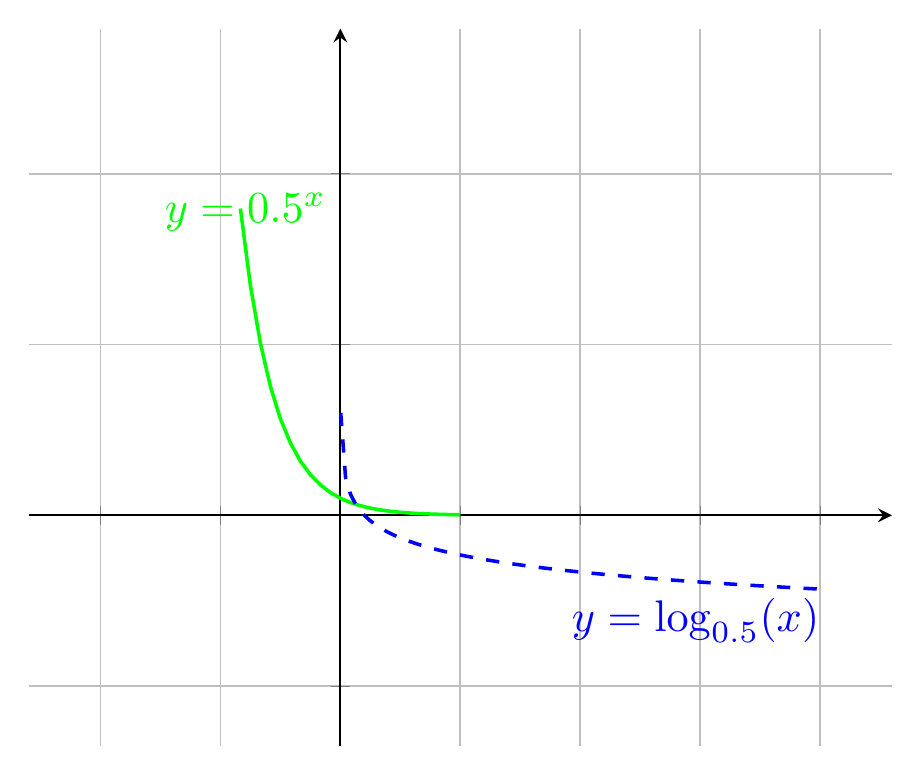
\begin{tikzpicture}[scale = 1.6]
	\begin{axis}[grid=both,
	xmin=-10,xmax=20,ymin=-10,ymax=25,
	yticklabels={,,},
	xticklabels={,,},
	axis lines=middle,
	restrict y to domain=-15:21,
	enlargelimits]
	\addplot[green, thick]  {pow(0.5,x)} node[pos=0.1, above]{$y=0.5^x$};
	\addplot[blue,domain=1/2^6:20,samples=100, thick, dashed]  {ln(x)/ln(0.5)} node[pos=0.8,below] {$y=\log_{0.5}(x)$};
	\end{axis}
	\end{tikzpicture}
	\caption{Plot of functions $y=\log_{0.5} x$ and $y=0.5^x$.}
	\label{fig:log_exp_0.5}
\end{figure}

	\begin{proposition}\label{prop:log_strict}
		Let $b, x_1, x_2$ be positive real numbers such that $b\neq 1$. Then
		\begin{enumerate}
			\item if $b>1$, $x_1>x_2$ if and only if $\log_b x_1 > \log_b x_2$,
			\item if $b<1$, $x_1>x_2$ if and only if $\log_b x_1 < \log_b x_2$.
		\end{enumerate}
	\end{proposition}
	
	\begin{proof}
		We illustrate the proof with two sample cases. In Figure \ref{fig:log_exp_2}, you can see the plot of $y=\log_2 x$ for $x \in [0, 10]$. As seen in the figure, logarithm to the base $2$ is strictly increasing. That is, if $x_1>x_2$, then $\log_2 x_1 > \log_2 x_2$. Now, let's prove that if $\log_2 x_1 > \log_2 x_2$, then $x_1>x_2$. In the same figure, you can see the plot of $y=2^x$, which is, again, strictly increasing. It means that for any two reals $x_1$ and $x_2$, if $x_1>x_2$, then $2^{x_1} > 2^{x_2}$. By definition, we can find positive reals $y_1$ and $y_2$ such that $x_1 = \log_2 y_1$ and $x_2=\log_2 y_2$. Now, the relation
		\begin{align*}
			x_1>x_2 \implies 2^{x_1} > 2^{x_2},
		\end{align*}
		transforms to
		\begin{align*}
			\log_2 y_1 > \log_2 y_2 \implies y_1 > y_2,
		\end{align*}
		which is what we wanted. Analogously, as shown in Figure \ref{fig:log_exp_0.5}, the functions $y=\log_{0.5} x$ and $y=0.5^x$ are both strictly decreasing and the proof of part $2$ is almost the same as the previous part.
		\end{proof}
	
\begin{figure}[t]
	\centering
	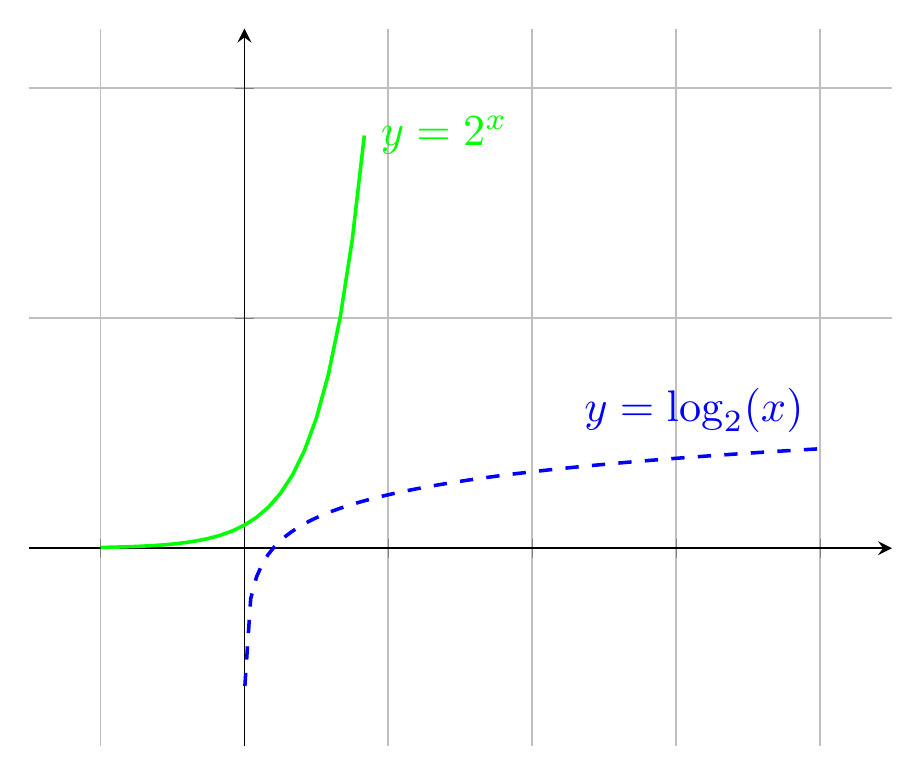
\begin{tikzpicture}[scale = 1.6]
	\begin{axis}[grid=both,
	xmax=20,ymax=20,
	yticklabels={,,},
	xticklabels={,,},
	axis lines=middle,
	restrict y to domain=-7:21,
	enlargelimits]
	\addplot[green, thick]  {pow(2,x)} node[right]{$y=2^x$};
	\addplot[blue,domain=1/2^6:20,samples=100,thick, dashed]  {ln(x)/ln(2)} node[above left] {$y=\log_2(x)$};
	\end{axis}
	\end{tikzpicture}
	\caption{Plot of functions $y=\log_2 x$ and $y=2^x$.}
	\label{fig:log_exp_2}
\end{figure}


\subsection{Number of Digits}
	There is a reason why we have explained logarithms in details even though they are part of elementary school teachings. A good number of students can not understand the meaning of logarithm properly. Let's show a problem so you realize what we mean.
	\begin{question}
		How many digits does $57$ have in base $2$?
	\end{question} 
	
	\begin{solution}
		First, think of a much simpler question: how many digits does $57$ have in base $10$? The answer is obviously $2$ digits. The reason is that any number between $10$ and $100$ has two digits in decimal system. In other words, the inequality $10<57<10^2$ tells us that $57$ has two digits in base $10$. 
		
		In general, in order to find number of digits of an integer $n$ in base $b$, we must find two consecutive powers of $b$ such that $n$ lies between them. In fact, if $b^m < n <b^{m+1}$, then $n$ has $m+1$ digits in base $b$.
		
		In case where $n=57$ and $b=2$, the required inequality is $2^5 < 57 <2^6$. Therefore, $57$ has six digits when written in binary. Indeed, $57 = (111001)_2$.
	\end{solution}
	We can now generalize this problem to the following proposition.
	\begin{proposition}
		Let $b$ and $n$ be integers bigger than $1$. Number of digits of $n$ when presented in base $b$ is $\lfloor \log_b n\rfloor +1$.
	\end{proposition}
	
	\begin{proof}
		As stated in the above solution, suppose that $m$ is the unique integer for which $b^m < n <b^{m+1}$. Then, the number of digits of $n$ in base $b$ is $m+1$. That is, it suffices to prove that $m=\lfloor \log_b n\rfloor$. Since $b$ is larger than $1$, we know from proposition \eqref{prop:log_strict} that logarithm to base $b$ is a strictly increasing function. This means that we can take logarithm to base $b$ from $b^m < n <b^{m+1}$ and the direction of the inequalities will not change. In other words,
		\begin{align*}
		\log_b b^m < \log_b n < \log_b b^{m+1},
		\end{align*}
		which gives $m<\log_b n<m+1$. Since $m$ is an integer, by definition of floor function, $m=\lfloor \log_b n \rfloor$.
	\end{proof}
	\section{Some Useful Facts}\label{sec:theoremsindiv}
	In this section, we provide some theorems which may help you solve problems more easily. Though you will find that we have emphasized not to be dependent on theorems or making them the core of solving problems, they help us a great deal and make our lives a lot easier. Therefore, you will find a lot of theorems in this book. But it does not mean in any way that theorems are the best way to improve in number theory. They merely help us speed up the process of solving problems. Nothing more. One could rediscover all the theorems while solving a problem and the end result would still be the same. The point is: you can get to the top of a mountain in many ways and the view is same. But the pleasure might be different based on the approach you take. If you use a helicopter to reach the peak of the mountain or climb all the way to the top. But definitely the latter approach brings you more pleasure. Anyway, we hope you understand our primary intention.
	
	\begin{theorem}\slshape
		Two integers $a$ and $b$ are of the same parity if and only if their sum and difference is even. Equivalently, they are of different parity if their sum and difference is odd.
	\end{theorem}
	
	\begin{corollary}\slshape\label{cor:sumparity}
		Exactly one of the two integers $a$ and $b$ is even if and only if $a\pm b$ is odd.
	\end{corollary}
	
	\begin{theorem}\slshape\label{thm:factorizeintopowersoftwo}
		Every positive integer $n$ can be written in the form $n=2^ks$, where $k$ is a non-negative integer and $s$ is an odd positive integer.
	\end{theorem}
	
	\begin{note}
		$ $
		\begin{enumerate}
			\item Here, $k$ is the largest power of $2$ that divides $n$. Therefore, $s$ must be odd. Moreover, $s$ is the largest odd divisor of $n$. Notice that if $n$ is odd, then $k=0$ and $s=n$.
			\item  One can write any positive integer $n$ as $n=p^ks$, where $p$ is a prime, $k$ is a non-negative, and $s$ is an integer coprime to $p$. The case $p=2$ (above theorem) is usually used in problem solving (and sometimes even in some combinatorics problems).
		\end{enumerate}
	\end{note}

	\begin{problem} 
		Let $n$ be a positive integer and let $S=\{1,2,\dots,2n\}$. Choose $n+1$ numbers $a_1,a_2,\dots, a_{n+1}$ out of $S$ so that
		\begin{align*}
			a_1<a_2<\dots <a_{n+1}.
		\end{align*}
		Prove that $a_i\mid a_j$ for some integers $1 \leq i,j \leq n+1$ with $i\neq j$.
	\end{problem} 
	
	\begin{solution}
		Write all members of $S$ in the form $2^{\a}\b$, where $\a$ is non-negative and $\b$ is the odd factor. There are exactly $n$ odd numbers among $1,2,\dots,2n$. Therefore, by pigeonhole principle\footnote{The pigeonhole principle states that if $n$ items are put into $m$ containers, with $n > m$, then at least one container must contain more than one item.}, among $n+1$ selected numbers $a_1,a_2,\dots, a_{n+1}$, there exist at least two numbers $a_i$ and $a_j$ (with $i\neq j$) which have the same odd factor. In other words,
		\begin{align*}
			a_i = 2^{\alpha_1}\beta \quad \text{and} \quad a_j = 2^{\alpha_2}\beta.
		\end{align*}
		Now, $a_i\mid a_j$ if $\alpha_1\leq \alpha_2$, and $a_j\mid a_j$ otherwise.
	\end{solution}
	
	\begin{theorem}\slshape
		Every composite positive integer $n$ can be written as $ab$ where $a$ and $b$ are coprime positive integers larger than $1$.
	\end{theorem}
	
	\begin{theorem}\slshape
		$(n-1)!$ is divisible by $n$ if and only if $n>4$ is a composite integer or $n=1$.\label{thm:cpfct}
	\end{theorem}
	
	\begin{proof}
		The case $n=1$ is trivial. For $n=2,3,4$ we can check by hand. For $n>4$, if $n$ is a prime, $n$ does not share a factor with any of $1,2,\dots,n-1$. Consequently, $n$ does not divide their product $(n-1)!$. If $n$ is composite, we can write $n=ab$ with $a$ and $b$ larger than $n$ and $a\neq b$. Since $a\neq b$ and $(n-1)!$ contains both $a$ and $b$ in the product, $n=ab|(n-1)!$.
	\end{proof}
	
	\begin{theorem}[Four Numbers Theorem]\slshape
		Let $a, b, c$, and $d$ be four positive integers such that $ab=cd$. Then there exist four positive integers $r,s,t$ and $u$ so that
		\begin{align*}
			a = rs, \quad b = tu, \quad	c = rt, \quad \text{and}\quad d = su.
		\end{align*}
	\end{theorem}
	
	\begin{proof}
		Let $(a,c)=g_1$. By proposition \eqref{prop:gcduncommon}, there exist integers $x_1$ and $y_1$ such that $a=g_1x_1$ and $c=g_1y_1$ with $x_1\perp y_1$. Also, let $(b,d)=g_2$, then there exist integers $x_2$ and $y_2$ such that $b=g_2x_2$ and $d=g_2y_2$ with $x_2\perp y_2$. Substitute these equations into the given equation $ab=cd$ to get
		\begin{align*}
			g_1g_2x_1x_2 & =g_1g_2y_1y_2,
		\end{align*}
		or simply $x_1x_2 =y_1y_2$. We claim that $x_1=y_2$ and $x_2=y_1$. To prove this claim, we use a trick. Observe that $x_1x_2=y_1y_2$ means $x_1 | y_1y_2$. The second part of Proposition \eqref{prop:cpdiv} tells us that since $x_1 \perp y_1$, we must have $x_1 | y_2$. With the same reasoning, one can show that $y_2|x_1$. It follows by proposition \eqref{prop:bothdivide} that $x_1 =y_2$. One can similarly show that $x_2=y_1$. Compare the  parameters in the theorem with the ones we just used and take $r=g_1, s=x_1, t=x_2 $, and $u=g_2$. The proof is complete.
	\end{proof}
	
	\begin{theorem}\slshape
		For positive integers $a, b, n$, and $e$, suppose that $a\perp b$ and $ab=n^e$. Then there exist positive integers $x$ and $y$ such that $a=x^e$ and $b=y^e$. In other  words, if product of two coprime positive integers is a perfect $e^{th}$ power, then both of them should be perfect $e^{th}$ powers. \label{thm:copower}
	\end{theorem}
	
	\begin{proof}
		Let us consider the prime factorization of $a$ and $b$ as the following.
		\begin{align*}
			a  = p_1^{e_1}\dots p_k^{e_k}\quad \text{and} \quad b = q_1^{f_1}\dots q_\ell^{f_\ell}.
		\end{align*}
		Then,
		\begin{align*}
			ab &= p_1^{e_1}\dots p_k^{e_k}q_1^{f_1}\dots q_\ell^{f_\ell}.\\
		\end{align*}
		From uniqueness of prime factorization, the only prime factors of $n$ must be $p_1,\dots,p_k$ and $q_1,\dots,q_\ell$. Let $n = p_1^{a_1}\dots p_k^{a_k}q_1^{b_1}\dots q_\ell^{b_\ell}$. Then
		\begin{align*}
			n^e  = p_1^{a_1e}\dots p_k^{a_ke}q_1^{b_1e}\dots q_\ell^{b_\ell e}.
		\end{align*}
		Since $ab=n^e$, we get
		\begin{align*}
			p_1^{e_1}\dots p_k^{e_k}q_1^{f_1}\dots q_\ell^{f_\ell} & = p_1^{a_1e}\dots p_k^{a_ke}q_1^{b_1e}\dots q_\ell^{b_\ell e}.
		\end{align*}
		The exponents of the primes in both sides must be equal. Therefore, $e_i=a_ie$ (for $i=1,2,\ldots,k$) and $f_j=b_je$ (for $j=1,2,\ldots,\ell$). Therefore, 
		\begin{align*}
			a = \Big(p_1^{a_1}\dots p_k^{a_k}\Big)^e \quad \text{and} \quad b = \left(q_1^{b_1}\dots q_\ell^{b_\ell}\right)^e,
		\end{align*}
		which proves the claim.
	\end{proof}
	
	\begin{note}
		You should think about why we considered the prime factorization and try to understand what led us into that way of thinking.
	\end{note}
	
	\begin{corollary}\slshape
		If $a$ and $b$ are relatively prime positive integers such that $ab$ is a perfect square, then $a$ and $b$ both are perfect squares.\label{cor:sqr}
	\end{corollary}
	
	\begin{theorem}\slshape
		Let $a,b$, and $c$ be positive integers such that $ab=c^2$. Then there exist integers $g,u,$ and $v$ with $u\perp v$ so that
		\begin{align*}
			a = gu^2,\quad b = gv^2, \quad \text{and} \quad c = guv.
		\end{align*}
	\end{theorem}
	
	\begin{proof}
		Let $g=(a,b)$. Then there exist coprime integers $x$ and $y$ such that $a=gx$ and $b=gy$. Then $g^2xy=c^2$ so that $g^2|c^2$, or $g|c$ (see the example provided right after proposition \eqref{prop:basicgcd} for a proof). This implies that there exists some positive integer $k$ for which $c=gk$. Substituting this into the equation, we find $k^2=xy$ with $x\perp y$. From corollary \eqref{cor:sqr}, there exist integers $u$ and $v$ such that $x=u^2$ and $y=v^2$. Thus, $a=gu^2,b=gv^2$, and $c=guv$.
	\end{proof}
	Now, we introduce a simple but really useful method for factorization: \textbf{Simon's Favorite Factorization Trick}\footnote{Named after Simon Rubinstein-Salzedo, a member of AoPS.}, or \textbf{SFFT} in brief.
	\begin{proposition}[SFFT]
		For any real numbers $x,y, j$, and $k$, the following relation holds:
		\begin{align*}
			xy+xk+yj+jk=(x+j)(y+k).
		\end{align*}
		Two special common cases are $$xy + x + y + 1 = (x+1)(y+1),$$ and $$xy - x - y +1 = (x-1)(y-1).$$
	\end{proposition}
	Let's see the motivation behind this trick. Once Mr. Simon was studying number theory, he found this problem: find all positive integers $x$ and $y$ such that $xy-x+y=49$. Simon probably hates expressions of this form because he cannot factorize them. However, if he adds $-1$ to both sides of his equation, he finds the nice and factored form $(x+1)(y-1)=48$, which is much easier to solve than the original equation. In fact, to solve the factorized equation, he only needs to find the divisors of $48$ (see theorem \eqref{thm:nos} for more details). If you look closely, SFFT is inspired by the so-called \textbf{Completing the Square Method}:
	\begin{align*}
		x^2+kx+\frac{k^2}{4}=\left(x+\frac{k}{2}\right)^2.
	\end{align*}
	In fact, the act of adding ${jk}$ to ${xy}+{xk}+{yj}$ in order to be able to factor it could be called \textbf{completing the rectangle} in analogy to the famous \textit{completing the square} trick.
	\begin{theorem}\slshape\label{thm:lcmfactor}
		If $N$ is the least common multiple of positive integers upto $n$, that is, $N=[1,2,\dots,n]$, then for a prime $p$, the maximum  integer $\a $ for which $p^\a |N$ is the unique non-negative integer $\a $ so that $p^\a \leq n<p^{\a +1}$. In other words, if $p_i$ is a prime less than or equal to $n$, and for that prime, $\a_i$ is the unique integer such that $p_i^{\a _i}\leq n<p_i^{\a _i+1}$ then,
		\begin{align*}
			N & = p_1^{\a _1}\dots p_k^{\a_i}.
		\end{align*}\label{thm:lcm}
		We can write $\a _i$ in terms of $n$ and $p_i$ using logarithm. Actually, $\a_i$ is the greatest non-negative integer less than or equal to $\log_{p_i}(n)$.
	\end{theorem}
	The proof in fact follows from the definition of least common multiple. Try some examples yourself and prove it. Also, we often use this kind of argument using logarithm to find some boundaries in some problems.
	
	\begin{theorem}\slshape
		The square of every odd integer leaves a remainder of $1$ when divided by $8$.
	\end{theorem}
	
	\begin{proof}
		We can write each odd integer $n$ in the form $n=2k-1$ for some $k\in\mathbb{Z}$. Then
		\begin{align*}
			n^2 = (2k-1)^2  = 4k^2-4k+1 = 4k(k-1)+1.
		\end{align*}
		Since one of $k$ or $k-1$ must be even (why?), we can write $k(k-1)=2\ell$ for some integer $\ell$. Then $n^2=8\ell+1$, and so $n^2$ leaves a remainder of $1$ when divided by $8$.
	\end{proof}
	
	\begin{theorem}\label{thm:4k+3prime}
		Every number of the form $4k+3$ has at least one prime factor of the form $4k+3$.
	\end{theorem}
	
	\begin{proof}
		The idea comes from the fact that if we multiply two numbers of the form $4k+1$, say $4a+1$ and $4b+1$, the result will be
		\begin{align*}
			(4a+1)(4b+1)=16ab+4a+4b+1=4(4ab+a+b)+1,
		\end{align*}
		which is, again, of the form $4k+1$. Clearly, all prime factors of a number $n$ of the form $4k+3$ are odd, and therefore are either of the form $4k+1$ or $4k+3$. If all prime factors of $n$ are of the form $4k+1$, then by the logic represented in above lines, any product of powers of these primes, including $n$, should be of the form $4k+1$. So, we get a contradiction and there exists at least one prime factor of $n$ which is of the form $4k+3$.
	\end{proof}
	\begin{theorem}\slshape\label{thm:nos}
		Let $n$ be a positive integer. The number of pairs $(a,b)$ of positive integers which satisfy the equation
		\begin{align*}
			ab & = n
		\end{align*}
		is $\tau(n)$, where $\tau(n)$ is the number of positive divisors of $n$.
	\end{theorem}
	
	The following example gives you an idea for the proof.
	
	\begin{example}
		Take $n=6$. The only positive divisors of $n$ are $1,2,3,$ and $6$. Therefore, $\tau(6)=4$. On the other hand, the equation $ab=6$ has exactly four solutions $(1,6), (2,3),(3,2)$, and $(6,1)$. 
	\end{example}
	
	We will study $\tau(n)$ in details in Chapter \ref{ch:arithfunc}.
	
	\begin{theorem}\slshape
		Every prime greater than $3$ is either of the form $6k+1$ or of the form $6k-1$.
	\end{theorem}
	
	\begin{proof}
		Consider an integer $n$. By definition \eqref{def:remainder}, the minimum absolute remainder $r$ of $n$ upon division by $6$ has the property that $|r| \leq 6/2=3$. In other words, $r$ can have the values $1,2,3,-1,-2$, and $-3$. For this reason, we can write an integer in exactly one of the following forms:
		\begin{align*}
			6k-2,6k-1,6k,6k+1,6k+2,6k+3.
		\end{align*}
		Numbers of the form $6k-2, 6k+2, 6k, 6k+3$ cannot be prime because the first two are divisible by $2$ and the last two are divisible by $3$. Thus, if $n$ is a prime, it must be either $6k-1$ or $6k+1$.
	\end{proof}
	Using the above theorem, we can prove the following.
	\begin{theorem}\slshape
		For a prime $p>3$, $24|p^2-1$.
	\end{theorem}
	
	\begin{proof}
		We can assume $p=6k\pm1$ for some integer $k$. So
		\begin{align*}
			p^2 = (6k\pm1)^2 = 36k^2\pm12k+1 = 12k(3k\pm1)+1.
		\end{align*}
		Note that $(k)+(3k\pm1)$ is odd. From corollary \eqref{cor:sumparity}, $k$ and $3k\pm1$ have different parity and $k(3k\pm1)$ is divisible by $2$. Let $k(3k\pm1)=2\ell$, then $p^2=24\ell+1$, or $p^2-1=24\ell$, which proves the theorem.
	\end{proof}
	
	\begin{theorem}\slshape
		If the sum of two positive integers is a prime, they are coprime to each other.
	\end{theorem}
	
	\begin{proof}
		Assume that $a+b=p$, where $p$ is a prime. If $(a,b)=g$ then there exist coprime positive integers $x$ and $y$ for which $a=gx$ and $b=gy$. So,
		\begin{align*}
			p = a+b = g(x+y),
		\end{align*}
		which means $g$ divides $p$. Since $p$ is a prime, its only divisors are itself and $1$. Hence, the only possible values for $g$ are $1$ and $p$. However, $g=p$ cannot happen since otherwise $x+y=1$ would lead to one of $x$ or $y$ being zero. Thus, $(a,b)=g=1$.
	\end{proof}
	
	
	\begin{theorem}\slshape\label{id:fatandthin}
		For any positive integer $n$,
		\begin{align*}
			a^n-b^n=(a-b)\Big(a^{n-1}+a^{n-2}b+\dots+b^{n-1}\Big).
		\end{align*}
		Furthermore, if $n$ is odd, then
		\begin{align*}
			a^n+b^n=(a+b)\Big(a^{n-1}-a^{n-2}b+\dots+b^{n-1}\Big).
		\end{align*}
		\label{thm:powDiv}
	\end{theorem}
	\begin{proof}
		We can just use induction on $n$, but we will try to avoid using induction as much as possible. For the first identity, define
		\begin{align*}
			S & =a^{n-1}+a^{n-2}b+\dots+b^{n-1}.
		\end{align*}
		Then, $aS=a^n+a^{n-1}b+\dots+b^{n-1}a$ and $bS=a^{n-1}b+a^{n-2}b^2+\dots+b^n$. Subtracting, we obtain
		\begin{align*}
			(a-b)S & =a^n-b^n,
		\end{align*}
		which finishes the proof. The second identity can be proved by using the first identity and the fact that when $n$ is odd, we have $a^n+b^n=a^n-(-b)^n$.
	\end{proof}
	
	\begin{corollary}\slshape
		\label{cor:a-b|a^n-b^n}
		Let $a$ and $b$ be any two integers. Then $a-b$ divides $a^n-b^n$ for all positive integers $n$. Also, $a+b$ divides $a^n+b^n$ for odd $n$.
	\end{corollary}
	
	
	\begin{theorem}\slshape\label{thm:powerdiv}
		Let $a,m,$ and $n$ be positive integers. Then, $a^m-1|a^n-1$ if and only if $m|n$.
	\end{theorem}
	
	\begin{proof}
		We will first show that if $m|n$, then $a^m-1|a^n-1$. Notice that if $m|n$, that there exists a positive integer $h$ such that $n=mh$, and so,
		\begin{align*}
			a^n-1 = a^{mh}-1 = \left( a^m\right)^h -1.
		\end{align*}
		Let $x=a^m$. By corollary \eqref{cor:a-b|a^n-b^n}, $x-1=a^m-1$ divides $x^h-1=a^n-1$, as desired.
		
		Let us now show the other side. If $a^m-1|a^n-1$, then,
		\begin{align*}
			a^m-1\mid a^n-1-(a^m-1)=a^n-a^m=a^m(a^{n-m}-1).
		\end{align*}
		Since $a^n-1\perp a^m$ (why?), we have $a^n-1\mid a^{n-m}-1$ by second part of proposition \eqref{prop:cpdiv}. Repeating the same process, we find $a^n-1\mid a^{n-2m}-1$. This suggests us to take $n=mq+r$ so that $0\leq r<m$. Then, we will have $a^n-1\mid a^{n-mq}-1=a^r-1$. Evidently, $a^r-1<a^m-1\leq a^n-1$, which forces $a^r-1=0$. So, $r=0$ and $n=mq$. The proof is complete.
	\end{proof}
	
	\begin{theorem}\slshape
		\label{thm:a^k-1prime}
		If $a^k-1$ is a prime for positive integers $a$ and $k>1$, then $a=2$ and $k$ must be a prime.
	\end{theorem}
	
	\begin{proof}
		As we already know,
		\begin{align*}
			a^k-1 & = (a-1)(a^{k-1}+a^{k-2}+\dots+a+1).
		\end{align*}
		If $a>2$, then $a-1$ will divide $a^k-1$ which is absurd because $a^k-1$ is a prime. So, $a$ must be $2$. Suppose that $k$ is composite. Then, $k=p\ell$ for some prime $p$ and integer $\ell>1$. Therefore,
		\begin{align*}
			a^k-1&=\left(a^p\right)^\ell -1\\
			&= (a^p-1)\left(a^{p(\ell-1)}+a^{p(\ell-2)}+\dots+1\right),
		\end{align*}
		which is impossible. Hence, $k$ must be a prime.
	\end{proof}
	
	\begin{remark}
		The numbers of the form $2^n-1$ are called \textit{Mersenne numbers} and denoted by $M_n$. According to the theorem, if $M_n$ is a prime, then $n$ must also be a prime.
	\end{remark}
	
	\begin{theorem}\slshape\label{thm:primec}
		Let $a$ and $k$ be positive integers. If $a^k+1$ is an odd prime, then $a$ is even and $k$ is a power of $2$.
	\end{theorem}
	
	See Problem \ref{prob:prime=poweroftwoplusone} for a proof.
	
	\begin{remark}
		For the particular case when $a=2$, the numbers $2^{2^n}+1$ are called \textit{Fermat numbers} and denoted by $F_n$. Notice that the reverse of the above theorem does \textit{not} hold. That is, not all Fermat numbers are primes. For instance,
		\begin{align*}
			F_5 = 2^{2^5}+1 = 4\, 294\, 967\, 297 = 641 \times 6\, 700\, 417.
		\end{align*}
	\end{remark}
	
	\begin{theorem}\slshape
		For two relatively prime positive integers $a$ and $b$,
		\begin{align*}
			(a^m-b^m,a^n-b^n)=a^{(m,n)}-b^{(m,n)}.
		\end{align*}
	\end{theorem}	
	
	\begin{proof}
		Here, we will use Euclidean algorithm as the idea is applicable to many similar problems. If $m=n$, the result is trivial since both sides are $a^m-b^m$. So, we can take $m>n$ without loss of generality\footnote{Wherever there is symmetry, don't forget to use this trick!}. Then we can write $m=n+k$ for some $k\in\N$. Therefore,
		\begin{eqnarray*}
			a^m-b^m & = & a^{n+k}-b^{n+k}\\
			& = & a^n(a^k-b^k)+b^k(a^n-b^n)
		\end{eqnarray*}
		Thus, by Euclidean algorithm,
		\begin{align*}
			(a^m-b^m,a^n-b^n) & = (a^n(a^k-b^k)+b^k(a^n-b^n),a^n-b^n)\\
			&=(a^n(a^k-b^k),a^n-b^n).
		\end{align*}
		Since $a$ and $b$ are coprime, $a^n\bot a^n-b^n$ (why?). This gives us
		\begin{eqnarray*}
			(a^m-b^m,a^n-b^n) & = & (a^n-b^n,a^k-b^k).
		\end{eqnarray*}
		Note that, this is the descending step of Euclidean algorithm! If we repeat the same process a couple of times, we would eventually reach $(m,n)$ in the exponent.
	\end{proof}
	
As a conclusion to this chapter, we define \textit{factorial} and \textit{binomial coefficient}.
	
		\begin{definition}[Factorial]
			Let $n$ be a positive integer. The \textit{factorial} of $n$, denoted by $n!$, is the product of all positive integers less than or equal to $n$. That is,
				\begin{align*}
					n! = 1 \times 2 \times \dots \times n.
				\end{align*}
			For convenience, we define $0!$ to be one\footnote{We can argue combinatorially as well, but let us put that aside for now.}.
		\end{definition}
		
		\begin{definition}[Binomial Coefficient]
			Let $n$ and $k$ be non-negative integers such that $k \leq n$. The \textit{Binomial Coefficient} indexed by $n$ and $k$ is denoted by $\displaystyle \binom{n}{k}$ (read ``\textit{$n$ choose $k$}'') and is equal to
				\begin{align*}
					\binom{n}{k} = \frac{n!}{k!(n-k)!}.
				\end{align*}
		\end{definition}
		
		\begin{note}
			It can be proved combinatorially that there are $\binom{n}{k}$ ways to choose $k$ elements, disregarding their order, from a set of $n$ elements. Although we may use this combinatorial fact in some problems, we only deal with the number theoric definition of binomial coefficients in this book.
		\end{note}
		
		\begin{proposition}
			The binomial coefficient is an integer.
		\end{proposition}
		
		\begin{hint}
			Use Problem \ref{prob:productdividesfactorial} in chapter \ref{ch:solved}.
		\end{hint}
	You are probably familiar with the \textit{binomial theorem}. We state this theorem here because of its high importance but do not prove it. Interested reader may see a proof of binomial theorem along with several useful related identities in Appendix \ref{ch:null}.
		\begin{theorem}[Binomial Theorem]\slshape
			For any positive integer $n$,
				\begin{eqnarray*}
					(a+b)^n & = & a^n+\binom{n}{1}a^{n-1}b+\binom{n}{2}a^{n-2}b^2+\dots+\binom{n}{1}ab^{n-1}+b^n.
				\end{eqnarray*}
		\end{theorem}
		
		\begin{theorem}\slshape\label{thm:binpdiv}
			Let $n$ be a positive integer. Then, $n$ is a prime if and only if $n$ divides $\binom{n}{k}$ for all $0<k<n$.
		\end{theorem}% requires the only if part.
		
	For now, we will be proving only the first part.
	
		\begin{proof}
			From identity number \ref{id:binomreduction} of theorem \eqref{thm:binom} in Appendix \ref{ch:null}, we know that
				\begin{align*}
					k\binom{p}{k} & = p\binom{p-1}{k-1}.
				\end{align*}
			Obviously, the right side is divisible by $p$, so must be the left side. From the definition of prime numbers, $p\bot k$. So, by the second part of the previous proposition, we can say $p$ must divide $\binom{p}{k}$.
		\end{proof}
	
\section{Solved Problems}	
	Well, now that we have a basic understanding of how divisibility relations work, it is the time to see how to apply those propositions to solve problems. Let us start with some really easy problems so that the reader has a firm idea about how to approach a problem. We will gradually discuss more difficult problems. Most importantly, we will not focus on how to use theorems to solve problems or implement them. We want to improve the intuitive ability of the reader instead.
	
		\begin{problem}
			Find all positive integers $n$ so that $n$ divides $n+3$.
		\end{problem}
		
	This can be solved in a variety of ways. Before we solve this, it would be pleasant to share some experience. This may not directly help readers understand how to solve the problem, but it may help them understand how different people think when they encounter a problem. 
	
	Masum was coaching a group of average students who barely had the idea of problem solving back in $2014$. After showing them some basic facts about divisibility, he threw this problem at them. Here is how they approached it: most of them started trial and error to find the solution. They were checking different values for $n$ to see if they satisfy the condition. Not all student could realize that this method will not work in general \textit{for all numbers} even if you find some initial solutions. One or two of the students went for the idea that if $n$ divides $n+3$, then $n+3$ is at least twice $n$. However, when increasing $n$, $2n$ becomes larger than $n+3$ after some $n$, and this leads to a solution. Another student solved the problem in the old fashioned way: by division process. That is, he divided $n+3$ by $n$ and found out that $n$ must divide $3$. Other than those few students, most of them got that $n=1$ and $n=3$ work but could not prove that these are the only solutions. In fact, that is the most difficult part of solving a number theory problem. 
	
	When you encounter a problem in mathematics, you probably come up with an assumption. For instance, in this problem, you may assume that the only solutions are $1$ and $3$. Most of the times our observations are true, but in many cases there are counter examples or some cases where our assumption fails. In our problem, if we just say the only solutions to the problem are $1$ and $3$ without proving it, we must tolerate comments such as ``How do you know there is not any large $n$ which is also a solution?'' That is why we have to prove everything we claim is true. Of course, if our claim is implied from a well-known theorem in mathematics, we can skip the proof and refer to the theorem. However, if the claim is totally new or relies on theorems which are not well known, we have to provide a proof. Obviously, the reader of your proof defines the famousness of the theorems you are allowed to use. There must be a huge difference in the way you solve a problem when you are explaining it to a math teacher or to a sixth grade student. By the way, when writing a solution to a problem at an olympiad test (or any other sophisticated exam), be careful not to consider every theorem obvious or well known. Whatever the problem is, try to prove every claim that you make.
	
	A suggestion: while reading a solution, try to find the motivation behind its idea rather than understanding it or learning the technique used in the solution. 
	
		\begin{solution}[Old-fashioned Way]
			Since $n|n+3$, the fraction $\dfrac{n+3}{n}=1+\dfrac{3}{n}$ is a positive integer. This shows that $\dfrac{3}{n}$ must be an integer. Therefore, $n$ divides $3$ and the only possible values for $n$ are $1$ and $3$.
		\end{solution}
		
		\begin{solution}[A Smarter Way]
			We know that if $a|b$ and $a|c$, then $a|b-c$. But how can we know what to subtract? If $m$ is a given constant, we can easily find all numbers $n$ such that $n|m$ just as in the previous solution. See that the right side of $n|n+3$ has a variable $n$ which is not constant. So, we need to remove it somehow. This is where divisibility rules come into play. We can now subtract $n|n$ from $n|n+3$ from to obtain $n|(n+3)-n=3$ or $n|3$. In words, $n$ is a divisor of $3$ which has namely two divisors $1$ and $3$. Thus, $n$ can be $1$ or $3$.
		\end{solution}
		
		\begin{solution}[Another Smart Solution]
			For positive integers $a$ and $b$, if $a|b$, $b\geq a$. Now, since $n+3$ cannot be equal to $n$, if it has to be divisible by $n$, it must be at least twice $n$, i.e., $n+3\geq2n$. This forces $3\geq n$ and so $n$ is one of $1,2$, or $3$. There are only three values so we can check them by hand and get the answer.
		\end{solution}
	Note the difference between the first and the second solution. There are pretty much no differences other than the fact that the latter is more systematic. You will eventually find that solving problems this way is particularly useful in Olympiads.
	
	For now, we will keep the use of inequality in store and solve a few problems by twisting up left and right sides of divisibility relations.
		\begin{problem}
			Find all $n \in \N$ so that $n|2n+3$.
		\end{problem}
		
		\begin{solution}
			This time we have to remove $n$ like before, but notice that there is an extra $2$ attached.
			
			We can overcome this easily: just see that $n|2n$ and then it is the same as the previous problem: $n|2n+3-2n=3$.
		\end{solution}
		
		\begin{problem}
			Find all $n \in \N$ so that $n+1\mid 3n+4$.
		\end{problem}
		
		\begin{solution}
			The left side contains more than just a $n$, but it does not make any difference. We have $n+1 \mid 3(n+1)=3n+3$ and it is given in the problem that $n+1 \mid 3n+4$. Subtracting,
				\begin{align*}
					n+1|3n+4-(3n+3)=1,
				\end{align*}
			which means $n+1$ must be $1$. This is impossible because $n+1$ is a positive integer greater than $1$.
		\end{solution}
		
		\begin{note}
			When dealing with a divisibility relation $k|m$ in which $m$ is constant, there are $\tau(m)$ possible values for $k$, where $\tau(m)$ is the number of positive divisors of $m$ (why?).
		\end{note}
	Try to do the following problem yourself before reading the solution.
		\begin{problem}
			Find all $n\in\N$ which satisfies $4n+2|6n+5$.
		\end{problem}
		
		\begin{solution}
			There are coefficients on both sides of divisibility now. Still it can be overridden but it is a bit tricky. See that $4n+2|3(4n+2)=12n+6$ and also $4n+2 \mid 2(6n+5)=12n+10$. Now that the coefficients are matched, we can subtract and find
				\begin{align*}
					4n+2|12n+10-(12n+6)=4.
				\end{align*}
			So, $4n+2$ must be one of $1,2$, or $4$. None of these values give a valid solution for $n$.
		\end{solution}
	If you have not noticed already, this idea can be generalized to find all $n$ satisfying $an+b|cn+d$, where $a,b,c,$ and $d$ are integers. Then what shall we multiply both sides with? Here is a hint: consider the $\lcm$ of $a$ and $c$. Why $a$ and $c$?
		\begin{problem}\label{prob:ex1}
			Find all positive integers $n$ for which $8n+9|12n+5$.
		\end{problem}
		
		\begin{solution}
			Our working principle is: we want to eliminate the variables on the right side so we get a constant value. That is, we want the right side to be a number, not a variable. In order to do this, we must construct two divisibility relations to subtract from each other and get a constant value. In other words, we have to find $a$ and $b$ such that the difference of right sides of $8n+9 \mid a(8n+9)$ and $8n+9 \mid b(12n+5)$ does not include $n$. So, the coefficients of $n$ must be equal in the two. The minimum value for this common coefficient will be the $\lcm$ of $8$ and $12$, which is $[8,12]=24$. Therefore, $a=3$ and $b=2$ and hence,
				\begin{align*}
					8n+9 & \mid 3(8n+9) =24n+27,\\
					8n+9 & \mid 2(12n+5) =24n+10.
				\end{align*}
			Thus, $8n+9\mid 24n+27-(24n+10)=17$ and $8n+9$ is either $1$ or $17$. The equation $8n+9=1$ does give a valid solution. So, the only solution is obtained from $8n+9=17$, which gives $n=1$.
		\end{solution}
		
		\begin{problem}[Dhaka Divisional Olympiad, 2010]
			Find all positive integers $n$ greater for which divides $n+4$ and $n+12$ for some positive integer $n$.
		\end{problem}
		
		\begin{solution}
			We are asked to find positive integers which would divide $n+4$ and $n+12$ both, no matter what. If $d$ is such a positive integer then
				\begin{align*}
					d|n+4 & , d|n+12\\
					\iff d|(n+12)&-(n+4)=8
				\end{align*}
			We immediately get that $d\in\{1,2,4,8\}$.
		\end{solution}
	
		\begin{problem}
			Find all primes $p$ so that $9p+1$ is also a prime.
		\end{problem}
		
		\begin{solution}
			This can be done easily considering parity. When you encounter a problem with primes (especially if you are asked to find a prime), it may be helpful to separate the problem into two cases. The first case is $p=2$ which works here. The second case is when $p$ is odd. It is trivial that as $p$ is odd, $9p+1$ is even. However, we want $9p+1$ be a prime. This is a contradiction because $9p+1$ is larger than $2$. Therefore, the only solution is $p=2$ for which $9p+1=19$ is also a prime.
		\end{solution}
		
		\begin{problem}
			Find all positive integers $n$ so that $7n+1\mid 8n+55$.
		\end{problem}
		
		\begin{solution}
			Since $[8,7]=56$, the two required relations would be
				\begin{align*}
					7n+1 & \mid 8(7n+1)=56n+8,\\
					7n+1 & \mid 7(8n+55)=56n+385.
				\end{align*}
			By subtracting, we find $7n+1\mid 377$. Now, we have to find divisors of $377$. When you are stuck with finding divisors, instead of trying random numbers or testing the numbers $2,3,4,5,\ldots$ serially to find if they divide $377$, try a more efficient approach which reduces your effort significantly. By proposition \eqref{factorsqrt}, if $n$ is composite, then it must have a prime factor less than or equal to $\sqrt{n}$.  Since $\sqrt{377} \approx 19.4$, it suffices to check which primes less than or equal to $19$ divide $377$. These primes are $2,3,5,7,11,13,17,19$. 
				\begin{itemize}
					\item $2 \nmid 377$ since the rightmost digit is odd,
					\item $3 \nmid 377$ since the sum of digits is $17$,
					\item $5 \nmid 377$ because the number ends in $7$,
					\item $7 \nmid 377$ because $377=7\cdot53+6$,
					\item $11 \nmid 377$ as the difference of sum of altering digits is $(3+7)-7=3$,
					\item $13 \mid 377$ because $37 + 4 \cdot 7 = 65 = 13 \cdot 5$.
				\end{itemize}
			So, we find the factorization of $377$ to be $377=13 \cdot 29$. This means that $7n+1$ is a divisor of $13 \cdot 29$. Notice that $7n+1$ is a number which leaves remainder $1$ when divided by $7$. Therefore, look for numbers among $13, 29, 13, $ and $377$ which leave a remainder of $1$ when divided by $7$. The only possibility is $7n+1=29$, which gives $n=4$.
		\end{solution}

		\begin{problem}\label{prob:n+3|n^2+2}
			Find all $n\in\N$ for which $n+3$ divides $n^2+2$.
		\end{problem}
	We should again remove the variables from the rights side of $n+3\mid n^2+2$. Here are two solutions for the problem.
		\begin{solution}[First Solution]
			 First, multiply $n+3$ by $n$ to get
				\begin{align*}
					n+3 \mid n^2+3n.
				\end{align*}
			Now, subtract this from the given relation to find
				\begin{align*}
					n+3 \mid 3n-2.
				\end{align*}
			The problem is now similar to the ones we solved earlier. In fact, subtracting
				\begin{align*}
					n+3 \mid 3n+9 \text{ and } n+3 \mid 3n-2,
				\end{align*}		
			we obtain $n+3|11$ which immediately gives $n=8$ as the only solution.
		\end{solution}
		
		\begin{solution}[Second Solution]
			This one is more elegant. In order to avoid the second step, we can directly multiply $n+3$ by $n-3$ to obtain
			\begin{align*}
				n+3  |n^2-9.
			\end{align*}
			Subtracting from the original relation, $n+3 \mid n^2+2-(n^2-9)$ or $n+3|11$, and we find the same solution as before.
		\end{solution}
		
		\begin{problem}
			Find the greatest positive integer $x$ for which
				\begin{align*}
					x+10|x^3+10.
				\end{align*}
		\end{problem}
	
		\begin{solution}
			Since $3$ is odd, we can use corollary \eqref{cor:a-b|a^n-b^n} to write $x+10 \mid x^3+10^3$. So,
				\begin{align*}
					x+10|(x^3+1000)-(x^3+10)=990,
				\end{align*}
			and the answer is $x=980$.
		\end{solution}
		
		\begin{problem}
			Find all positive integers $n$ so that $n^6+n^4$ is divisible by $7n+1$.
		\end{problem}
		
		\begin{solution}
			How do we approach this problem? One idea is to go ahead like we did in the first solution of problem \eqref{prob:n+3|n^2+2}, by eliminating powers of $n$ one by one. Here is a better solution.
			
			First write it as, $7n+1 \mid n^4(n^2+1)$. The problematic part is $n^4$. Many beginners make mistakes in such situations claiming that $7n+1$ does not divide $n^4$, and so $7n+1 \mid n^2+1$. This is \textbf{wrong}. In general, the following statement is wrong: 
			\begin{displayquote}
				For positive integers $a,b$, and $c$, if $a|bc$ and $b$ is not divisible by $a$, then $a|c$.
			\end{displayquote}
			This is another common  mistake new problem solvers make. You can check this using an example: $14$ divides $28=7\times4$ but $14$ does not divide $7$. But in this problem, we can still take $n^4$ off because $n^4$ is coprime to $7n+1$. Just notice that $7n+1$ leaves a remainder of $1$ when divided by $n$, so $n\perp7n+1$. Evidently, $n^4\perp7n+1$ by part $4$ of proposition \eqref{prop:cpdiv}. Using part $2$ of the same proposition, we can cancel out $n^4$ and get 
				\begin{align*}
					7n+1  \mid n^2+1.
				\end{align*}
			Multiply $n^2+1$ by $49$ to find $ 7n+1 \mid 49n^2+49$. On the other hand, $7n+1$ divides $(7n+1)(7n-1)=49n^2-1$, and so,
				\begin{align*}
					7n+1 \mid (49n^2+49)-(49n^2-1) = 50.
				\end{align*}
			Note that $7n+1$ leaves a remainder of $1$ when divided by $7$. Therefore, we look for divisors of $50$ which leaves a remainder $1$ when divided by $7$. The divisors of $50$ are $1,2,5,10,25$, and $50$. Only $1$ and $50$ leave the desired property among these numbers. Since $n$ is a positive integer, $7n+1\geq7\cdot1+1=8$. Therefore, $7n+1=50$ or $n=7$.
		\end{solution}
		
		\begin{remark}
			We could handle the last part in another way. Write $7n+1\mid (n^2+1)-(7n+1)$, so that
				\begin{align*}
					7n+1  \mid n^2-7n \implies 7n+1\mid  n(n-7).
				\end{align*}
			Again, $n\perp7n+1$ implies $7n+1|n-7$. If $n=7$, we have a solution. Otherwise, $7n+1$ would have a larger value than $|n-7|$ and we get a contradiction.
		\end{remark}
		
		\begin{problem}
			If $ax+by=1$, find $(a,b)$.\label{prob:d1}
		\end{problem}
		
		\begin{solution}
			Assume that $(a,b)=g$. Then we can find two coprime integers $m$ and $n$ so that $a=gm$ and $b=gn$. Setting these into the given equation, we observe $g(mx+ny)=1$. This implies that $g$ divides $1$, and so $g=1$.
		\end{solution}
		
		\begin{note}
			We can similarly show that $(x,y)=(x,b)=(a,y)=1$.
		\end{note}
		
		\begin{problem}
			Find the number of solutions to the equation
			\begin{align*}
				\dfrac{1}{x}+\dfrac{1}{y}=\dfrac{1}{2015}
			\end{align*}
			in positive integers.
		\end{problem}
		
		\begin{solution}
			We can rewrite the equation as
				\begin{align*}
					\dfrac{x+y}{xy} & = \dfrac{1}{2015}.
				\end{align*}
			Multiplying both sides by $2015xy$, we find $xy=2015(x+y)$. This can be represented as
				\begin{align*}
					(x-2015)(y-2015) & = 2015^2.
				\end{align*}
			According to theorem \eqref{thm:nos}, we get that the number of solutions is the number of positive divisors of $2015^2$, $\tau(2015^2)$. 
		\end{solution}
		
		\begin{note}
			Did you realize that this was actually SFFT? And what do you think the result would be if we considered solutions in integers (not necessarily positive)?
		\end{note}
		
		\begin{problem}
			Find all $n\in\N$ such that $2^n+n|8^n+n$.
		\end{problem}
		
		\begin{solution}
			There is $8$ on the right side and $2$ on the left side. Since $8=2^3$, this should certainly provoke us to use the fact that $a+b|a^3+b^3$. In this case,
				\begin{align*}
					2^n+n   & \mid (2^n)^3+n^3 \\
					\implies  2^n+n & \mid 8^n+n^3\\
					\implies 2^n+n	& \mid (8^n+n^3)-(8^n+n)\\
					\implies 2^n+n & \mid n^3-n.
				\end{align*}
			Now we need to find all $n$ such that $2^n+n\mid n^3-n$. If you play around with the small values of $n$, you will clearly see that $2^n$ grows a lot faster than $n^3$. Since $2^n+n|n^3-n$, we must have
				\begin{align*}
					2^n+n & \leq n^3-n.
				\end{align*}
			The following lemma gives us the limit we need for $n$. Once again, you have to prove it. You can use induction to do so (can you use logarithm?).
				\begin{lemma}
					For $n>9$, the inequality $2^n+n>n^3-n$ holds.
				\end{lemma}
			By the lemma, if $n>9$, there are no solutions. Now we are left with a few possibilities for $n$ because $n$ must be less than or equal to $9$. We can easily check by hand that there are no solutions for this case as well.
		\end{solution}
		
		\begin{problem}[IMO 1959, Problem 1]
			Prove that for any integer $n$, the fraction $$\dfrac{14n+3}{21n+4}$$ is irreducible.
		\end{problem}
	
	\begin{solution}
		We must make sense of the problem first. It asks to prove that a fraction is irreducible. That means the fraction cannot be simplified anymore. In other words, we must prove that the numerator ($14n+3$) and denominator ($21n+4$) of the fraction are coprime to each other. How do we prove this? We will show this in two ways: 
		\begin{enumerate}
			\item Let $g=(14n+3,21n+4)$. Then,
			\begin{align*}
				g & \mid 14n+3,\\
				g & \mid 21n+4.
			\end{align*}
		We already know we have to prove that $g=1$. So, let us try to remove the $n$ on the right side. Since $[14,21]=42$ and $42=14\cdot3=21\cdot2$, we can make use of the following two relations:
			\begin{align*}
				g & \mid 3(14n+3) = 42n+9,\\
				g & \mid  2(21n+4)= 42n+8.
			\end{align*}
		Thus, $g|(42n+9)-(42n+8)=1$ and $g=1$.
		
			\item Take $14n+3=gx$ and $21n+4=gy$ for some integers $x$ and $y$. Note that $3(14n+3)-2(21n+4) = 1$, and so
			\begin{align*}
				 3gx-2gy  & = 1,
			\end{align*}
		or $g(3x-2y) = 1.$ So, $g|1$ and this gives us the same result $g=1$.
		\end{enumerate}
	\end{solution}
	
	\begin{remark}
		You should understand that both solutions are essentially the same, but with different approaches or thinking styles.
	\end{remark}
	
	\begin{problem}\label{prob:prime=poweroftwoplusone}
		Show that if a prime is of the form $2^n+1$, then $n=2^m$ for some integer $m$.
	\end{problem}
	
	\begin{solution}
		According to theorem \eqref{thm:factorizeintopowersoftwo}, write $n=2^ms$, where $s$ is an odd positive integer. By theorem \eqref{id:fatandthin}, we can write
			\begin{align*}
				p = 2^n+1 &= 2^{2^{m}s}+1 = \left(2^{2^{m}}\right)^s+1\\
				   		  &=\left(2^{2^m}+1\right)\left(2^{2^{m}(s-1)}+2^{2^{m}(s-2)}+ \cdots + 2^{2^{m}}+1\right).
			\end{align*}
		Clearly, as $p$ is a prime, this is impossible unless $s=1$. So $n=2^m$.
	\end{solution}
	
	\begin{problem}
		Find all integer solutions to the equation
			\begin{align*}
				a(b+1)+b(c+1)+c(a+1)+abc=0.
			\end{align*}
	\end{problem}
	
	\begin{solution}
		Yes, this looks similar to \textbf{SFFT}. It has three variables instead of two, so we cannot directly use Simon's trick. However, if you already learned the motivation behind that trick, the form of the problem does not matter. Here, $1$ is missing! Add it to both sides to get
			\begin{align*}
				abc+ab+bc+ca+a+b+c+1=1.
			\end{align*}
		The left hand side shows you how SFFT looks like for three variables. Try to compute $(a+j)(b+k)(c+\ell)$ and remember it. You will soon realize that the left hand side of the above equation factors as $(a+1)(b+1)(c+1)$. Therefore,
			\begin{align*}
				(a+1)(b+1)(c+1)=1.
			\end{align*}
		The rest of the solution is just case work. If the product of three integers equals $1$, what can they be? The solutions are
			\begin{align*}
				(a,b,c)=(0,0,0), (-2,-2,0), (-2,0,-2), (0,-2,-2).
			\end{align*}
	\end{solution}
	
	\begin{problem}[Turkey TST 2014, Day 2, Problem 4]
		Find all odd positive integers $m$ and $n$ such that
			\begin{align*}
				n\mid 3m+1 \mbox{ and } m\mid n^2+3.
			\end{align*}
	\end{problem}
	
	\begin{solution}
		Do not panic! Even some TST problems can be solved using simple tricks. The general idea is to first see if there are infinitely many solutions. Check some numbers and some special values for $m$ and $n$. For instance, put $m=n$ to see if it fits in. In this problem, we cannot find a pattern to construct infinitely many solutions, so we guess that there are finite solutions and continue. To be honest, many of such divisibility problems (with finite solutions) rely heavily on case working, and you need to know how to start the case work. One of the best ways to handle this situation is to find a limit for $m$ and $n$. Remember the properties of divisibility from proposition \eqref{prop:basicdiv}. Limit means boundary, and boundary means inequality (see part 10 of that proposition). Actually, we will use the fact that if $a|b$ for positive integers $a$ and $b$, then $a \leq b$. After we have found the limit, the case work begins.
		
		Write $n|3m+1$ as $3m+1=nk$ or $m=\frac{nk-1}{3}$. Now try to rewrite the second divisibility relation as
			\begin{align*}
				& \frac{nk-1}{3} \bigg| n^2 + 3 \\
				\stackrel{\times 3}{\implies} & nk-1\mid 3n^2+9 \\
				\stackrel{\times k}{\implies} & nk-1\mid 3n^2k+9k.
			\end{align*}
		On the other hand, we know that $nk-1|3n(nk-1)=3n^2k-3n$. Subtract these two last divisibility relations to find
			\begin{align*}
				nk-1 \mid 3n+9k,
			\end{align*}
		which in turn implies $nk-1 \leq 3n+9k$. This inequality can be simplified using \textbf{SFFT} in this way:
			\begin{align*}
				nk-3n-9k\leq 1 \stackrel{\text{add }27}{\implies} (n-9)(k-3) \leq 28.
			\end{align*}
		Notice that we have found the limit we wanted! The solution is almost obvious from here on, because one can manually put all possible values for $n$ and $k$ such that $(n-9)(k-3) \leq 28$ and pick those which satisfy the problem conditions ($n|3m+1$ and $m|n^2+3$). In order to avoid this tedious endeavor, we start a proper case work.
		
		We start case work on the parameter $k$ (you will know why). Since $m$ is odd and $3m+1=nk$, $k$ is even. We check some possible values of $k$:
			\begin{enumerate}[(a)]
				\item If $k=2$, then from $nk-1\mid 3n+9k$ we have $2n-1\mid 3n+18$, and thus
					\begin{align*}
						2n-1|2(3n+18)-3(2n-1)=39.
					\end{align*}
				 This means that $2n-1=1, 3, 13$, or $39$. None of these values make a solution for the problem.
				
				\item If $k=4$, then from $nk-1|3n+9k$ we have $4n-1|3n+36$, and thus
					\begin{align*}
						4n-1|4(3n+36)-3(4n-1)=147.
					\end{align*}
				This means that $4n-1=1, 3, 7, 21, 49$, or $147$. Checking the values of $n$, we find that $n=1$ and $n=37$ satisfy the conditions of the problem and give us the solutions $(m,n)=(1,1)$ and $(m,n)=(49,37)$.
				
				\item If $k\geq 6$, then the inequality $(n-9)(k-3) \leq 28$ can be transformed to
					\begin{align*}
						(n-9) \leq \frac{28}{k-3} \leq \frac{28}{3},
					\end{align*}
				which means $n\leq 9+28/3$. Since $n$ is a positive integer, the latter inequality simplifies to $n \leq 18$ (why?). Also, $n$ is odd, so we have to check only the numbers $n=1, 3, 5, 7, 9, 11, 13, 15$, and $17$. In this case, only $n=13$ gives a valid solution (check it) and it is $(m,n)=(43,13)$.
			\end{enumerate}
		Finally, the solutions are
			\begin{align*}
				(m,n)=(1,1), (49,37), (43,13).
			\end{align*}
	\end{solution}
\newpage
\section{Exercises}
	
	
	\begin{problem}
		Find all pairs of positive integers $(x, y)$ for which
			\begin{align*}
				\frac{x^2+y^2}{x-y}
			\end{align*}
		is an integer that divides $1995$.
	\end{problem}
	
%		\begin{solution}
%			Say $d=\gcd(x,y)$, $x=da$, $y=db$, $\gcd(a,b)=1$. Then $\dfrac{x^2+y^2}{x-y} = \dfrac{d(a^2+b^2)}{a-b}$. But $\gcd(a-b,a^2+b^2) \mid 2$, since $a^2+b^2 = (a-b)^2 + 2ab$ and $\gcd(a-b,ab) =1$. Therefore $a-b \mid 2d$, so $2d = c(a-b)$, and finally we need $c(a^2+b^2) \mid 2\cdot 1995 = 2\cdot 3\cdot 5\cdot 7\cdot 19$. This forces $a^2+b^2 \in \{5,10\}$, so $\{a,b\} \in \{\{1,2\}, \{1,3\}\}$. Thus the solutions come from these pairs, and any $d \mid 3\cdot 7\cdot 19$.
%			
%		\end{solution}
	
	\begin{problem}
		Let $x, y$, and $z$ be integers such that
			\begin{align*}
				(x-y)^2+(y-z)^2+(z-x)^2 = xyz.
			\end{align*}
		Prove that $(x+y+z+6)$ divides $(x^3+y^3+z^3)$.
	\end{problem}
	
%		\begin{solution}
%			Plugging $(x-y)^2+(y-z)^2+(z-x)^2=xyz$ into the identity $x^3+y^3+z^3-3xyz$ $=\frac{1}{2}(x+y+z)((x-y)^2+(y-z)^2+(z-x)^2)$ yields $x^3+y^3+z^3-3xyz$ $=\frac{1}{2}(x+y+z)(xyz)$. Call this $(*)$.  Now if all of $x,y,z$ are odd then $(x-y)^2+(y-z)^2+(z-x)^2$ $=xyz$ cannot hold (just check mod $2$ to get $0\equiv 1\pmod 2$ -- contradiction), thus one of $x,y,z$ is even. Let's say (WLOG) that $x$ is even, so $x=2x_1$. Substituting this into $(*)$ gives $x^3+y^3+z^3-6x_1yz$ $=(x+y+z)(x_1yz)$ $\Rightarrow x^3+y^3+z^3$ $=x_1yz(x+y+z+6)$, so that $x^3+y^3+z^3$ is clearly divisible by $x+y+z+6$. Done.
%		\end{solution}
	
	\begin{problem}
		Let $k$ and $m$, with $k > m$, be positive integers such that the number $km(k^2 - m^2)$ is divisible by $k^3 - m^3$. Prove that $(k - m)^3 > 3km$. %24
	\end{problem}
	
%		\begin{solution}
%			\textit{First Solution.} Let $(k,m)=(ga,gb)$ where $g=\gcd(k,m)$ (and $a>b$). Now $k^3-m^3|km(k^2-m^2)\implies a^3-b^3|gab(a^2-b^2)\implies a^2+ab+b^2|gab(a+b)$.\\ Suppose there exists a prime $p$ such that $p|a^2+ab+b^2$ and $p|ab(a+b)$. So $p$ divides one of $a,b,a+b$. If $p|a$ then $p|a^2+ab$ but also $a^2+ab+b^2$ i.e. $p|b^2$, a contradiction since $a,b$ are coprime. Same goes for the case $p|b$. \\
%			
%			If $p|a+b$ then $p|(a+b)^2=a^2+2ab+b^2$. Then $p|a^2+2ab+b^2-(a^2+ab+b^2)=ab$ so we are back to $p$ dividing one of $a,b$, which we have seen to be impossible. Hence $\gcd(a^2+ab+b^2,ab(a+b))=1$ so $a^2+ab+b^2|g$ -  this implies $g\ge a^2+ab+b^2$.\\ Now $a^2+ab+b^2>3ab$ by AM-GM ($a\not= b$) so that $(a^2+ab+b^2)(a-b)^3>3ab$ since $(a-b)$ is positive and at least one. But $g(a-b)^3\ge (a^2+ab+b^2)(a-b)^3>3ab\implies g^3(a-b)^3>3g^2ab$ i.e. $(k-m)^3>3km$.\\
%			
%			\textit{Second Solution.} If $k^3-m^3|km(k^2-m^2)$, then dividing by $k-m$ we have $k^2+km+m^2|km(k+m)=k^2m+km^2$. \\
%			Trivially, $k^2+km+m^2|k(k^2+km+m^2)=k^3+k^2m+km^2$, which implies $k^2+km+m^2|k^3$. Similarly, $k^2+km+m^2|m^3$.
%			Let $gcd(k,m)=d$. Since then $gcd(k^3,m^3)=d^3$, there exists a linear combination $Ak^3+Bm^3=d^3$. Hence $k^2+km+m^2|d^3$.\\
%			But then $k^2+km+m^2|d^3\left(\frac kd-\frac md\right)^3=(k-m)^3$. Since these are positive numbers, this means that $(k-m)^3$ cannot be smaller than $k^2+km+m^2$, therefore $(k-m)^3\ge k^2+km+m^2>3km$.
%		\end{solution}
	
	\begin{problem}
		Let $F(n) = 13^{6n+1} + 30^{6n+1} + 100^{6n+1} + 200^{6n+1}$ and define
			\begin{align*}
				G(n) = 2F(n) + 2n(n - 2)F(1) - n(n - 1)F(2).
			\end{align*}
		Prove by induction that for all integers $n \geq 0$, $G(n)$ is divisible by $7^3$. %42
	\end{problem}
	
	\begin{problem}
		Prove that for every integer $n \geq 2$, there exist $n$ different positive integers such that for any two of these integers $a$ and $b$, $a+b$ is divisible by $a - b.$ %109
	\end{problem}
	
%		\begin{solution}
%			We build such sets inductively.
%			$\{1,2\}$ is a set with two elements with the given property.\\
%			Suppose we have a set $S_n=\{a_1<...<a_n\}$ with the given property.
%			Let $N,k,m$ be positive integers satisfying the following:
%			$N$ is divisible by all of the pairwise differences in $S_n$\\
%			$k>N+(a_n-a_1)$ and $k!>a_1$
%			$$\frac{k!-a_1}{N}<m\le\frac{k!+k-a_n}{N}.$$
%			
%			We claim that the set $S_{n+1}=\{k!,a_1+mN,a_2+mN,...,a_n+mN\}$ has the given property.
%			It is easy to see that $\{a_1+mN,a_2+mN,...,a_n+mN\}$ has the given property by the definition of $N$.
%			If $x\in S_{n+1}-\{k!\}$ then $0<x-k!\le k$ and hence $(x-k!)|k!\Rightarrow (x-k!)|(x+k!)$.
%		\end{solution}
	
	\begin{problem}[Iran Second Round 1994]
		Let $\overline{a_1a_2a_3\ldots a_n}$ be the representation of a $n-$digits number in base $10.$ Prove that there exists a one-to-one function like $f : \{0, 1, 2, 3, \ldots, 9\} \to \{0, 1, 2, 3, \ldots, 9\}$ such that $f(a_1) \neq 0$ and the number $\overline{ f(a_1)f(a_2)f(a_3) \ldots f(a_n) }$ is divisible by $3.$ %141
	\end{problem}
	
%		\begin{solution}
%			Let digit $i$ appears $x_i$ times in the number, for $i=0,1,2,\ldots,9$. By pigeonhole principle, there exist $x_i,x_j,x_k$ which are congruent in modulo 3.\\ Among the remaining seven integers $\{x_0,x_1,\ldots,x_9\}-\{x_i,x_j,x_k\}$ by pigeonhole principle there exist $x_l,x_m,x_n$ which are congruent in modulo 3.\\ Therefore $x_i+x_j+x_k-x_l-x_m-x_n\equiv0\pmod3$. So we can define the following function: $f(i)=1$, $f(j)=4$, $f(k)=7$, $f(l)=2$, $f(m)=5$, $f(n)=8$, and the other digits are randomly assigned the values 0, 3, 6, 9. Thus we have $$f(a_1)+f(a_2)+\ldots+f(a_n)\equiv x_i+4x_j+7x_k+2x_l+5x_m+8x_n\equiv0\pmod3,$$ i.e., $3|\overline{f(a_1)f(a_2)\ldots f(a_n)}$.\\
%			Edit: I forgot the $f(a_1)\ne0$ part. But we can simply interchange the values 0, 3, 6, 9.
%		\end{solution}
	
	\begin{problem}[Slovenia 2010]
		Let $a,b$, and $c$ be three positive integers. Prove that $a^2+b^2+c^2$ is divisible by $4$ if and only if $a,b$, and $c$ are all even. %148
	\end{problem}
	
%		\begin{solution}
%			If $a,b,c$ are even then indeed $a^2 +b^2 +c^2 \equiv 0 \pmod 4$. \\
%			
%			Now assume that $a^2 +b^2 +c^2 $ is divisible by $4$, but not all the numbers are even. Then we'd have two of the numbers being odd, say $a$ and $b$. Let $a=2k+1$, $b=2q+1$ and $c=2p$, then we'd have: $a^2 +b^2 +c^2=4k^2 +4k +1 +4q^2 +4q +1 +4p^2 $ which is clearly not divisible by $4$. Hence contradiction.
%		\end{solution}
	
	\begin{problem}[ILL 1990, THA1]
		Let $m$ be an odd positive integer not divisible by $3$. Prove that
			\begin{align*}
				\big\lfloor 4^m -(2+\sqrt 2)^m \big\rfloor
			\end{align*}
		is divisible by $112.$ %196
		
		Note: for any real number $x$, $\lfloor x \rfloor$ is the largest integer not exceeding $x$.
	\end{problem}
	
	\begin{hint}
		Show that each term is equal to $4^m-(2+\sqrt 2)^m-(2-\sqrt 2)^m$.
	\end{hint}
	
%		\begin{solution}
%			Let the sequence $a_n$ defined as:\\
%			$a_1=0$\\
%			$a_2=4$\\
%			$a_3=24$\\
%			$a_{n+3}=8a_{n+2}-18a_{n+1}+8a_n$ $\forall n>0$\\
%			
%			It's easy to show that $a_n=4^n-(2+\sqrt 2)^n-(2-\sqrt 2)^n$ and since $1>(2-\sqrt 2)^n>0$ $\forall n>0$ and $a_n\in\mathbb Z$ $\forall n$, we get:
%			$$\left\lfloor4^n-(2+\sqrt 2)^n\right\rfloor=a_n \quad \forall n>0.$$
%			Looking then at $a_n$ modulus $112$, we get $\{0,4,24,8,$ and the repeated cycle $0,48,0,32,80,64\}$. Hence the required result.
%		\end{solution}
	
	\begin{problem}
		Let $P_n = (19 + 92)(19^2 +92^2) \cdots(19^n +92^n)$ for each positive integer $n$. Determine, with proof, the least positive integer $m$, if it exists, for which $P_m$ is divisible by $33^{33}.$ %264
	\end{problem}
	
	
	\begin{problem}
		Prove that we can choose $2^n$ numbers from $2^{n+1}$ positive integers such that their sum is divisible by $2^n$. %334
	\end{problem}
	
	\begin{problem}[Baltic Way 1993]
		Prove that for any odd positive integer $n$, $n^{12}-n^8-n^4+1$ is divisible by $2^9$. %381
	\end{problem}
	
%		\begin{solution}
%			This quantity is $(n^4+1)(n^2+1)^2(n^2-1)^2$ and $2|n^4+1$ and $2^2|(n^2+1)^2$ and $2^6|(n^2-1)^2$.
%		\end{solution}
	
	\begin{problem}
		Let $m$ and $n$ be two positive integers. Does there exist positive integers $a,b$, and $c$ all greater than $m$ such that $abc$ is divisible by $a+n$, $b+n$, and $c+n$? %389
	\end{problem}
	
%		\begin{solution}
%			Yes. Take $a=n(\lambda^2-1),b=c=n\lambda$ and take $\lambda$ arbitrarily large.\\
%			
%			Heuristics:
%			Taking $a,b,c$ as multiples of $n$ is intuitive as we can factor $a+n$ as $n(p+1)$ etc where $\frac{1}{n}(a,b,c)=(p,q,r)$. Then we need $p+1|n^2qr,q+1|n^2rp,r+1|n^2pq$.\\
%			
%			It could prove useful to ignore the $n^2$ and just find numbers $p,q,r$ such that $p+1|qr,q+1|rp,r+1|pq$. Take $p$ as the maximum of $p,q,r$. Then my first idea was to take $p+1=qr$. Then $q+1|rp=r(qr-1)=qr^2-r$. So $qr^2=r\pmod{q+1}\implies r(r+1)=0\pmod{q+1}$. So $q+1|r$ or $q+1|r+1$. Similarly $r+1|q$ or $r+1|q+1$.\\
%			
%			If $q+1|r$ then $q<r$ so $q<q+1<r+1$ but this contradicts $r+1|q$ or $r+1|q+1$. So $q+1|r+1\implies q\le r$. Similarly we can't have $r|q+1$ so $r+1|q+1$ and so $r\le q$. So $q=r$. Then $p=qr=q^2$. Plugging this back in obtains a valid formula for $a,b,c$.
%		\end{solution}
	
	\begin{problem}[Baltic Way 1997]
		Prove that in every sequence of $79$ consecutive positive integers written in the decimal system, there is a positive integer whose sum of digits is divisible by $13$. %465
	\end{problem}
	
%		\begin{solution}
%			Consider consecutive numbers $n,n+1,n+2,...,n+k-1$. Let $a=n\mod 100$. If $a\le 60$, then among $k\le 49$  we have $13|s(n+i)$. Else we get to $a=00=(n+m)\mod 100, m<40$ and among $n+m,n+m+1,...n+m+39$ we get $N$, suth that $13|s(N)$. Obviosly $N\le n+(139-61)=n+78$. Therefore $k\le 79.$
%		\end{solution}
	
	\begin{problem}[Baltic Way 2006]
		A $12-$digit positive integer consisting only of digits $1,5$, and $9$ is divisible by $37$. Prove that the sum of its digits is not equal to $76$\watermark. %508
	\end{problem}
	
%		\begin{solution}
%			Suppose such an integer with sum of digits equals 76 exists. Note that 111111111111 is divisible by 37, so we can reduce each digit by 1, the number now have the following property: It consists only of digits 4 and 8, at most 12 digit, and the sum of digits equals 64. Since $\gcd(4,37)=1$, we can divide the integer by 4, so it consists only of digits 1 and 2, the sum of digits is 16.\\
%			
%			Note that $10^3\equiv1\pmod{37}$. So if we divide the digits into four groups of 3 consecutive digits, the sum of these 3-digit numbers is still divisible by 37. This integer is 7 mod 9 and 0 mod 37, so it must be 259, 592, or 925. But the largest possible digit is 8, we get a contradiction.
%		\end{solution}
	
	\begin{problem}
		Prove that the number $19^{1976} + 76^{1976}$
			\begin{enumerate}
				\item is divisible by the (Fermat) prime number $F_4 = 2^{2^4} + 1$, and
				\item is divisible by at least four distinct primes other than $F_4$.
			\end{enumerate}
	\end{problem}
	
%		\begin{solution}
%			For part (b), we need to use a lemma that $gcd(2^{a}+1,2^{b}+1)=2^{gcd(a,b)}+1$, where $a,b$ is odd number.\\
%			$Proof:$ This is because $gcd(2^{a}+1,2^{b}+1)$ is a factor of $gcd(2^{2a}-1,2^{2b}-1) =2^{2gcd(a,b)}-1 =[2^{gcd(a,b)}-1][2^{2gcd(a,b)}+1]$
%			As $gcd(2^{a}+1,2^{gcd(a,b)}-1)=1$ $gcd(2^{b}+1,2^{gcd(a,b)}-1)=1$
%			Therefore $gcd(2^{a}+1,2^{b}+1)$ is a factor of $2^{gcd(a,b)}+1$
%			Also we know that $2^{gcd(a,b)}+1$ divides $2^{a}+1,2^{b}+1$
%			Therefore $gcd(2^{a}+1,2^{b}+1)=2^{gcd(a,b)}+1$ where $a,b$ is odd number.\\
%			
%			It is easy to see that $19$ is one of the factors.
%			Actually, $2^{13}+1,2^{19}+1,2^{13.19}+1$ are also the factors.\\
%			By using the fact, we know that $2^{13.19}+1$ has factors other than $2^{13}+1,2^{19}+1$. And $gcd(2^{13}+1,2^{19}+1)=3$.\\
%			The last thing we need to show is that $19$ does not divide $2^{13}+1,2^{19}+1,2^{13.19}+1$, which is easily shown by Fermat's Theorem.
%		\end{solution}
	
	\begin{problem}
		Show that $5^{n} -4n+15$ is divisible by $16$ for all positive integers $n$.
	\end{problem}
	
%		\begin{solution}
%			For $n=1$ since $5^n-4n+15=16$ is divisible by $16$.
%			If the problem true with $n=k \in \mathbb{N}$, it means $5^k-4k+15$ is divisibly by $16$.\\
%			We need to prove the problem true with $n=k+1$.
%			We have $5^{k+1}-4(k+1)+15=5 \left( 5^k-4k+15 \right)+16k+64$ is divisible by $16$.
%		\end{solution}
	
	\begin{problem}
		Prove, without using mathematical induction, that  $5^{2n+2} -24 n -25$ is divisible by $576$.
	\end{problem}
	
	
	\begin{problem}[IMO 1979, Problem 1]
		If $p$ and $q$ are positive integers so that
			\begin{align*}
				\frac{p}{q}=1-\frac{1}{2}+\frac{1}{3}-\frac{1}{4}+ \dots -\frac{1}{1318}+\frac{1}{1319},
			\end{align*}
		prove that $p$ is divisible with $1979$. %760
	\end{problem}
	
%		\begin{solution}
%			We first write
%			\begin{align*}
%			\frac{p}{q}
%			&=1-\frac{1}{2}+\frac{1}{3}-\frac{1}{4}+\cdots-\frac{1}{1318}+\frac{1}{1319}\\
%			&=1+\frac{1}{2}+\cdots+\frac{1}{1319}-2\cdot\left(\frac{1}{2}+\frac{1}{4}+\cdots+\frac{1}{1318}\right)\\
%			&=1+\frac{1}{2}+\cdots+\frac{1}{1319}-\left(1+\frac{1}{2}+\cdots+\frac{1}{659}\right)\\
%			&=\frac{1}{660}+\frac{1}{661}+\cdots+\frac{1}{1319}
%			\end{align*}
%			Now, observe that
%			\begin{align*}
%			\frac{1}{660}+\frac{1}{1319}=\frac{660+1319}{660\cdot 1319}=\frac{1979}{660\cdot 1319}
%			\end{align*}
%			and similarly $\frac{1}{661}+\frac{1}{1318}=\frac{1979}{661\cdot 1318}$ and $\frac{1}{662}+\frac{1}{1317}=\frac{1979}{662\cdot 1317}$, and so on. We see that the original equation becomes
%			\begin{align*}
%			\frac{p}{q}
%			=\frac{1979}{660\cdot 1319}+\frac{1979}{661\cdot 1318}+\cdots+\frac{1979}{989\cdot 990}=1979\cdot\frac{r}{s}
%			\end{align*}
%			where $s=660\cdot 661\cdots 1319$ and $r=\frac{s}{660\cdot 1319}+\frac{s}{661\cdot 1318}+\cdots+\frac{s}{989\cdot 990}$ are two integers. Finally consider $p=1979\cdot\frac{qr}{s}$, and observe that $s\nmid 1979$ because $1979$ is a prime, it follows that $\frac{qr}{s}\in\mathbb{Z}$. Hence we deduce that $p$ is divisible with $1979$.
%		\end{solution}
	
	\begin{problem}[ILL 1970--1973, FIN1]
		Prove that $2^{147}-1$ is divisible by $343.$ %839
	\end{problem}
	
%		\begin{solution}
%			This is just $7^3|2^{3\cdot 7^2}-1=7\cdot (8^{7^2-1}+8^{7^2-2}+\ldots+8+1)$. This is equivalent to $7^2|8^{7^2-1}+8^{7^2-2}+\ldots+8+1$. The RHS is a sum consisting of $7^2$ terms, all of them being $1\pmod 7$, so it's divisible by $7^2$.
%		\end{solution}
	
	\begin{problem}[ISL 1998, NT7]
		Prove that for each positive integer $n$, there exists a positive integer with the following properties:
			\begin{itemize}
				\item It has exactly $n$ digits.
				\item None of the digits is zero.
				\item It is divisible by sum of its digits.
			\end{itemize}
	 %854
	\end{problem}
	
%		\begin{solution}
%			We prove by induction.\\
%			First we prove for $ 3^k$ digits. In this case we claim $ 3^k$ $ 1$s will satisfy the sequence.\\
%			$ 111 = 37*3$, so it is true for $ k = 1$. Assume it is true for $ k$. Then $ 3^k|\frac {10^{3^k} - 1}{9}$. So we need to prove $ 3^{k + 1}|\frac {10^{3^{k + 1}} - 1}{9} = (\frac {10^{3^k} - 1}{9})(10^0 + 10^k + 10^{2k})$. We have $ 3^k$ divides what is in the first parentheses, and $ 3$ divides what is in the second, since the sum of the digits of it is $ 3$. so $ 3^{k + 1}$ divides this and we are done.\\
%			
%			Now consider the $ q$ digit long number between $ \frac {10^{3^k} - 1}{9}$ and $ \frac {10^{3^{k - 1}} - 1}{9}$ which works. We construct a number of $ q - 1$ digits which works. We claim subtracting a multiple of $ m = 10^{3^k - r} - 10^{3^k - r - 3^{k - 2}}$ preserves both the sum of the digits and the property that the number is divisible by its digits, where $ r-1$ is the number of digits less than $ 3^k$ we have.\\
%			
%			Indeed, it is clear that subtracting $ m$ (or a multiple of $ m$) preserves the sum of the digits, since it increases one digit by one and decreases another by $ 1$.\\
%			
%			Also, $ 3^k$ divides our number to start with by the inductive hypothesis, and
%			$ 3^k|10^{3^k - r} - 10^{3^k - r - 3^{k - 2}}$ is equivalent to
%			$$ 3^k|10^{3^{k - 2}} - 1.$$
%			But this is clear since we established above that $ 3^k|\frac {10^{3^k} - 1}{9}$.\\
%			
%			We will never be forced to add $ 1$ to a digit which is already $ 9$, since we can terminate the process when all digits are $ 9$, which is when there are $ 3^{k - 1}$ digits.\\
%			This is because $ \frac {3^k}{3^k - r - (3^k - 3^{k - 2} - r)} = 9$, so when each time we remove the front digit we add to the digit $ 1/9$th of the length of the original number along from the digit we subtracted, meaning we will end with $ 3^{k - 2}$ $ 9$s.\\
%			
%			So our construction is essentially as follows: look at a number of $ q$ digits with first digit $ s$ which works. subtract $ m$ $ s$ times. We now have a number of $ q - 1$ digits which works. (This fails for $ k = 1$ and $ k = 0$ since we use $ 3^{k - 2}$, but it is trivial to contruct examples for these cases)\\
%			
%			\noindent For the $ 11111111$ example we have\\
%			$ 111111111$\\
%			$ 21111111$\\
%			$ 3111111$\\
%			$ 411111$\\
%			$ 51111$ (e.g. here $ r=5$, $ k=2$)\\
%			$ 6111$\\
%			$ 711$\\
%			$ 81$\\
%			$ 9$ \\
%			(although we can stop when we reach $ 6111$ since $ 3$ digits is already a power of $ 3$)
%		\end{solution}
	
	\begin{problem}[ISL 1998, NT1]
		Determine all pairs $(x,y)$ of positive integers such that $x^{2}y+x+y$ is divisible by $xy^{2}+y+7$. %894
	\end{problem}
	
%		\begin{solution}
%			\textit{First Solution.} 
%			If $(xy^2+y+7)|(x^2y+x+y)$, then there exists a positive integer $k$  such that $k(xy^2+y+7) = x^2y+x+y$ , or
%			$$7k-y = (xy+1)(x-ky).$$
%			
%			First we claim that all solutions have both sides nonnegative.
%			
%			Suppose $7k-y < 0$ . But then we have
%			
%			$|7k-y| < |y| < |xy+1| < |xy+1||x-ky|$,
%			
%			which is a contradiction. So both sides are nonnegative. Now consider the two cases: (1) both sides are zero, and (2) both sides are positive.\\
%			
%			\textbf{Case 1:} Both sides are zero.
%			
%			Then we have $7k-y = 0 \Rightarrow y = 7k$ . And also $(xy+1)(x-ky) = 0$, but since $xy+1 > 0$ we know $x-ky = 0 \Rightarrow x = ky = 7k^2$ . So we have all solutions of the form $(x,y) = (7k^2, 7k)$ .\\
%			
%			\textbf{Case 2:} Both sides are positive.
%			
%			Then $x > ky$ so the RHS is positive. So we have $7k > 7k-y = (xy+1)(x-ky) > (xy+1) > y^2k+1$. Hence $y < 3$ . So we check $y = 1, 2$.
%			
%			For $y = 1$ , we have $(x+8)|(x^2+x+1)$. Since
%			$$\frac{x^2+x+1}{x+8} = x-7+\frac{57}{x+8},$$
%			we have $(x+8)|57 \Rightarrow x = 11, 49$ , giving the solutions $(11,1)$ and $(49,1)$.\\
%			
%			For $y = 2$ , we have $(4x+9)|(2x^2+x+2) \Rightarrow (4x+9)|(4x^2+2x+4)$ . Since
%			$$\frac{4x^2+2x+4}{4x+9} = x-\frac{7x-4}{4x+9},$$
%			so $(4x+9)|(7x-4)$ . But since $2(4x+9) > 7x-4$ , we must have $4x+9 = 7x-4$ , which does not have an integer solution.\\
%			
%			Hence our only solutions are $(x,y) = (11,1); (49,1); (7k^2, 7k)$ for positive integers $k$.
%			
%			\textit{Second Solution.} 
%			$xy^2+y+7 \mid x^2y+x+y$
%			$\Rightarrow xy^2+y+7 \mid y(x^2y+x+y)-x(xy^2+y+7)$
%			$\Rightarrow xy^2+y+7 \mid y^2-7x$\\
%			
%			Clearly $y^2-7x <xy^2+y+7$ so $y^2-7x=0$ which gives $(x,y)=(7t^2,7t)$ ot $y^2-7x <0$.This gives $7x-y^2 \ge xy^2+y+7 \Rightarrow (x+1)y^2+y+7-7x \le 0 \Rightarrow y \le 2$.$y=2 \Rightarrow 4x+9 \mid 2x^2+x+2 \Rightarrow 4x+9 \mid 4x^2+2x+4-4x^2-9x \Rightarrow 4x+9 \mid 7x-4 \Rightarrow 4x+9 \mid 7(4x+9)-4(7x-4)=79 \Rightarrow$ no solution.\\
%			For $y=1$ we have
%			$x+8 \mid x^2+x+1 \Rightarrow x+8 \mid x^2+x+1 -x^2-8x \Rightarrow x+8 \mid 7x-1 \Rightarrow x+8 \mid 7(x+1)-(7x-1) \Rightarrow x+8 \mid 57 \Rightarrow \boxed{x=11,49}$.\\
%			
%			\textbf{Solutions:} $(x,y)=(7t^2,7t),(11,1),(49,1)$.
%		\end{solution}
	
	\begin{problem}[Ukrain TST‌2008, P6]
		Prove that there exist infinitely many pairs $ (a, b)$ of natural numbers not equal to $ 1$ such that $ b^b + a$ is divisible by $ a^a + b$.
	\end{problem}
	
%		\begin{solution}
%			$ (a,b)=(a,a^{2a-2}-a^{a}+1)$ also work for $ a>1$ being of the form $ 4k+1$, where $ k$ is an integer. After easy calculations we have to prove that $ a^{2a-2}+1|a^{a(a^{2a-2}-a^{a}+1)-1}-1$, which will be proved if we show that $ 2(2a-2)|a(a^{2a-2}-a^{a}+1)-1$, but it's equivalent to $ 4(a-1)|(a-1)(1+a^{a-3}+a^{a-2}+...+a+1)$, or $ 4|1+a^{a-3}+a^{a-2}+\cdots+a+1$, but this holds as $ a=4k+1$,from which the desired conclusion follows.
%		\end{solution}
	
	\begin{problem}[Japan Final Olympiads 2009, P1]
		Find all positive integers $n$ such that $8^n + n$ is divisible by $2^n + n$.  %1187
	\end{problem}
	
%		\begin{solution}
%			$ x^3 + y^3 = (x + y)(x^2 - xy + y^2) \implies 2^n + n|8^n + n^3 \implies 2^n + n | 8^n + n^3 - (8^n + n) = n^3 - n$.\\
%			And it implies that $ n^3 - n = 0$ or $ |n^3 - n| \ge 2^n$.
%			The first case gives $ n = 1$, which is a solution.\\
%			The second case: for $ n \ge 10$, $ 2^n > n^3 > n^3 - n$, by induction: $ 1024 > 1000$, and $ 2^n > n^3$ implies that $ 2^{n + 1} > 2n^3 \ge (n + 1)^3$ because $ 3n^2 + 3n + 1 \le 3n^2 + 3n^2 + 3n^2 = 9n^2 < n^3$ for $ n \ge 10$.
%			So we only need to consider $ 2 \le n \le 9$. The valid solutions are $ n = 2,4,6$. When we include the 1st case, the set of solutions is $ n = 1,2,4,6$. 
%		\end{solution}
%		
	
	\begin{problem}[Romania JBMO TST‌2001]
		Determine all positive integers $a,b,c$, and $d$ in the order $a<b<c<d$ with the property that each of them divides the sum of the other three. %471
	\end{problem}
	
%		\begin{solution}
%			So $(a+b+c)=kd$ but $a+b+c<3d$ and so $k\in\{1,2\}$.\\
%			1) $k=1$ and $d=a+b+c$\\
%			Then $c|a+b+(a+b+c)$ and so $c|2(a+b)$ and $2(a+b)=k_1c$ but $2(a+b)<4c$ and so $k_1\in\{1,2,3\}$\\
%			1.1) $k_1=1$ and $c=2(a+b)$\\
%			The numbers are $a,b,2a+2b,3a+3b$\\
%			And $b|6a+5b$ and so $b|6a$ and, $a|6b$\\
%			Let then $a=a_1u$ and $b=b_1u$ with $a_1<b_1$ coprime.\\
%			We get $b_1|6$ and $a_1|6$ and so $(a_1,b_1)$ is $(1,2),(1,3),(1,6),(2,3),(2,6),(3,6)$\\
%			And solutions :\\
%			$(a,b,c,d)=(u,2u,6u,9u)$\\
%			$(a,b,c,d)=(u,3u,8u,12u)$\\
%			$(a,b,c,d)=(u,6u,14u,21u)$\\
%			$(a,b,c,d)=(2u,3u,10u,15u)$\\
%			
%			
%			1.2) $k_1=2$ and $c=a+b$\\
%			The numbers are $a,b,a+b,2a+2b$\\
%			And $b|4a+3b$ and so $b|4a$ and $a|4b$\\
%			Let then $a=a_1u$ and $b=b_1u$ with $a_1<b_1$ coprime.\\
%			We get $b_1|4$ and $a_1|4$ and so $(a_1,b_1)$ is $(1,2),(1,4)$\\
%			And solutions :\\
%			$(a,b,c,d)=(u,2u,3u,6u)$\\
%			$(a,b,c,d)=(u,4u,5u,10u)$\\
%			
%			1.3) $k_1=3$ and $c=\frac{2a+2b}3$\\
%			The numbers are $a,3t-a,2t,5t$ with $2t<2a<3t$\\
%			And $a|10t-a$ and so $a|10t$ and $10t=ak'$ and since $\frac{20}3a<10t<10a$, we get $10t=7a$ or $10t=8a$ or $10t=9a$\\
%			$10t=7a$ implies $t=7p$ and $a=10p$ and the numbers are $(10p,11p,14p,35p)$ which is not a solution\\
%			$10t=8a$ implies $t=4p$ and $a=5p$ and the numbers are $(5p,7p,8p,20p)$ which is not a solution\\
%			$10t=9a$ implies $t=9p$ and $a=10p$ and the numbers are $(10p,17p,18p,45p)$ which is not a solution\\
%			
%			2) $k=2$ and $d=\frac{a+b+c}2$\\
%			Then $c|a+b+\frac{a+b+c}2$ and so $\frac 32(a+b)+\frac c2=k_1c$ and so $\frac 32(a+b)=(k_1-\frac 12)c$\\
%			And since $a+b<2c$, we get $k_1<3+\frac 12$ and so $k_1\in\{1,2,3\}$\\
%			
%			
%			2.1) $k_1=1$ and $c=3(a+b)$\\
%			Then $d=2(a+b)<c$ and so no solution\\
%			
%			2.2) $k_1=2$ and $c=a+b$\\
%			Then $d=a+b=c$ and so no solution\\
%			
%			2.3) $k_1=3$ and $5c=3(a+b)$\\
%			The numbers are $a,5t-a,3t,4t$ with $4t<2a<5t$\\
%			So $a|12t-a$ and so $a|12t$ and so $12t=k_2a$ but $\frac{24}5a<12t<6a$ and so $12t=5a$\\
%			The numbers are $(12p,13p,15p,20p)$ which is not a solution.\\
%			
%			Hence the set of basis solutions (all other are obtained thru multiplication by any positive integer) :\\
%			$(a,b,c,d)=(1,2,3,6)$\\
%			$(a,b,c,d)=(1,2,6,9)$\\
%			$(a,b,c,d)=(1,3,8,12)$\\
%			$(a,b,c,d)=(1,4,5,10)$\\
%			$(a,b,c,d)=(1,6,14,21)$\\
%			$(a,b,c,d)=(2,3,10,15)$
%		\end{solution}
	
	\begin{problem}[BrMO 2003, Modified]
		Determine all triples $(x,y,z)$ of integers greater than $1$ with the property that $x$ divides $yz-1$, $y$ divides $zx-1$ and $z$ divides $xy-1$. %521
	\end{problem}
	
%		\begin{solution}
%			WLOG $x\ge y\ge z>1$.\\
%			Now $\frac{xy-1}{z},\frac{yz-1}{x},\frac{zx-1}{y}$ are all integers, hence so is their product, i.e.
%			$$xyz|(xy-1)(yz-1)(zx-1)=x^2y^2z^2-x^2yz-x^2yz-xy^2z-xyz^2+xy+yz+zx-1.$$
%			Therefore $xyz|xy+yz+zx-1\implies xyz\le xy+yz+zx-1<xy+yz+zx\le 3xy$ hence $2<z$, which implies $z=2$.\\
%			Then back to the divisibility relation we have $2xy|xy+2x+2y-1$ so that $xy<2x+2y\le 4y\implies xy\le 4x\implies y\in\{2,3\}$.\\
%			If $y=2$ then $2=y|zx-1=2x-1$, a contradiction. Hence $y=3$ so that $x|yz-1=6-1=5\implies x=5$.\\
%			
%			Hence the sole solution $(2,3,5)$ for integers greater than $1$.
%		\end{solution}
	
	\begin{problem}[All Russian Olympiads, P10.7]
		Positive integers $x>1$ and $y$ satisfy the equation $2x^2-1=y^{15}$. Prove that 5 divides $x$. %822
	\end{problem}
	
%		\begin{solution}
%			Suppose what they want is not true. Of course, 2 divides $y+1$ and if we write the equation as $ ((y^5+1)/2)( y^{10}-y^5+1)=x^2$ we observe that $ ((y^5+1)/2, y^{10}-y^5+1)$ is a divisor of 3. If it is 1, then $y^{10}-y^5+1$ is a perfect square, impossible for y at least 2 (we can put it between two consecutive squares). So, suppose it is 3. Then we can write $ y^5+1=6A^2$ and $y^{10}-y^5+1=3B^2$ with $x=3AB$. Since $ y^5-y$ is a multiple of 3, it follows that $ y+1$ is a multiple of 6. Thus, if we write $ ((y+1)/6)(y^4-y^3+y^2-y+1)=A^2$ we see that since 5 does not divide $A$, we have $ ((y+1)/6, y^4-y^3+y^2-y+1)=1$ and thus $ y^4-y^3+y^2-y+1$ is a square. Again, this is impossible by the fact that $ (2y^2-y)^2<4(y^4-y^3+y^2-y+1)<(2y^2-y+2)^2$.
%		\end{solution}
	
	\begin{problem}
		Find all pairs $(a,b)$ of positive integers such that $2a-1$ and $2b+1$ are coprime and $a+b$ divides $4ab+1.$ %1113
	\end{problem}
	
%		\begin{solution}
%			The answer $(a,b)=(n,n+1)$ for every integer $n$.\\
%			It is clear from the fact $a+b|4ab+1$ that $a+b|(2a+1)(2b+1)$ and $a+b|(2a-1)(2b-1)$.\\
%			Now let $gcd(2a-1,a+b)=g$.Hence $g|2(a+b)$ and $g|2a-1$ implies that $g|2b+1$ which contradicts our assumption that $gcd(2a-1,2b+1)=1$. So $gcd(a+b,2a-1)$ and therefore $a+b|2b-1$. But $2b+1<2(a+b)$. Hence $2B+1=2a+2b$, and thus $b=a+1.$\\
%			Now it is clear that then $a+b|4ab+1$. Again $gcd(2a-1,2b+1)=gcd(2b+1,4)=1$. Thus every pair of this form satisfies the condition.\\
%			So answer is $(a,b)=(n,n+1) \quad \forall$ $n$.
%		\end{solution}
	
	
	%==================================================
	%GCD-LCM

	\begin{problem}
		Determine all pairs $(m, n)$ of positive integers such that $m>n$ and
			\begin{align*}
				1 = \gcd(n+1,m+1) = \gcd(n+2,m+2) = \dots = \gcd(m,2m-n).
			\end{align*}
	\end{problem}
	
%	\begin{solution}
%		If $m-n \geq 2$, one of the numbers $n+1,n+2,\ldots,n+(m-n) = m$ will be divisible by $m-n$; say it's $n+k$. But then $m+1=(n+1) + (m-n)$ will also be divisible by $m-n$, so $m-n \mid \gcd(n+k,m+k)$, forcing $\gcd(n+k,m+k) \geq m-n > 1$. Thus the only possibility is $m=n+1$, for which it is trivial.
%		\\
%		There are just too many expressions. A more interesting question is if we stop at $\gcd(m-1,2n-m-1)=1$ (with $m>n+1$). Then the answer is $n=kp, m=kp+p$, with $p$ prime.
%	\end{solution}


	\begin{problem}
		Let $a_1,a_2,\ldots,a_n,\ldots$ be any permutation of all positive integers. Prove that there exist infinitely many positive integers $i$ such that $\gcd(a_i,a_{i+1})\leq \frac{3}{4} i$. %73
	\end{problem}

%	\begin{solution}
%		\textit{First Solution.} Assume the contrary. For sufficiently large $i$, we have $(a_i,a_{i+1})\le\frac34i$. Take a large number $b$ and let $k$ be the smallest positive integer not contained in $a_1,a_2,\ldots,a_b$. Let $p$ be the integer such that $a_p=k$ and $q$ be the smallest positive integer such that the sequence $a_1,a_2,\ldots,a_q$ contains $1,2,\ldots,2k-1$.\\
%		
%		Since $a_1,a_2,\ldots,a_b$ contains $1,2,\ldots,k-1$, then $b\ge k-1$. It is also clear that $p>b$, hence $p\ge k$.\\
%		
%		\textbf{Claim}: If $p\le r<r+1\le q$, then $\max\{a_r,a_{r+1}\}\ge2k$.\\
%		
%		Proof: Suppose the contrary, let $(a_r,a_{r+1})=l$. We have $l>\frac34r\ge\frac34p\ge\frac34k$. But $a_r$ and $a_{r+1}$ are multiples of $l$ and less than $2k$. Since $3l>\frac94k>2k$, then $a_r$ and $a_{r+1}$ must be $l$ and $2l$. So $l$ does not appear in $a_1,a_2,\ldots,a_b$, which implies $l\ge k$ and hence $2l\ge 2k$. Therefore one of $a_r$ and $a_{r+1}$ is not less than $2k$, a contradiction. The proof of claim is done. $\Box$\\
%		
%		Therefore, among $a_p,a_{p+1},\ldots,a_q$, there are at most $\frac{q-(p-1)+1}2=\frac{q-p}2+1$ numbers which are less than $2k$. Since $a_1,a_2,\ldots,a_q$ contains $1,2,\ldots,2k-1$, then \[2k-1\le p-1+\frac{q-p}2+1=\frac{p+q}2\] Using $k>\frac34p$ and $2k-1>\frac34q$, we get $p\le\frac{4k-1}3$ and $q\le\frac{4(2k-1)-1}3=\frac{8k-5}3$, so $\frac{p+q}2\le2k-1$. Equality must hold, so $p=\frac{4k-1}3,q=\frac{8k-5}3,a_q=2k-1$. We also conclude that $a_1,a_2,\ldots,a_{p-1},a_p,a_{p+2},a_{p+4},\ldots,a_q$ are less than $2k$.\\
%		
%		Since $1,2,\ldots,2k-2$ appears in $a_1,a_2,\ldots,a_{q-1}$ and $a_q=2k-1$, using the same argument as above, we conclude that $a_1,a_2,\ldots,a_{q-1}$ must be less than $2(2k-1)=4k-2$.\\
%		
%		Now note that $(a_p,a_{p+1})>\frac34p=\frac{4k-1}4$, so $(k,a_{p+1})\ge k$, equality must hold, so $k|a_{p+1}$. But $a_{p+1}<4k-2$. So $a_{p+1}=2k\text{ or }3k$.\\
%		
%		If $a_{p+1}=2k$, then $(2k,a_{p+1})>\frac34(p+1)=\frac{4k+2}4>k$, so $(2k,a_{p+2})=2k$ and $a_{p+2}>2k$, a contradiction.\\
%		
%		Hence $a_{p+1}=3k$. We have $(3k,a_{p+2})>\frac34(p+1)>k$. Hence $(3k,a_{p+2}=\frac{3k}2$ and hence $a_{p+2}=\frac{3k}2$. Finally, we have $(a_{p+2},a_{p+3})>\frac34(p+2)$. Hence $(\frac{3k}2,a_{p+3})>\frac{4k+5}4>k$, hence $(\frac{3k}2,a_{p+3})=\frac{3k}2$. But $a_{p+3}$ cannot be equal to $a_{p+1}=3k$, hence $a_{p+3}\ge3\cdot\frac{3k}2>4k-2$, a contradiction. And we are finally done.\\
%		
%		\textit{Second Solution.} Assume for the sake of contradiction that there exists a positive integer $N$ such that $\gcd(a_i,a_{i+1})>3i/4\forall{i\ge N}$, and let $M=\max(a_1,\ldots,a_{N-1})$. We will repeatedly use the fact that $\min(a_i,a_{i+1})\ge 1+\lfloor{3i/4}\rfloor$ and $\max(a_i,a_{i+1})\ge 2+2\lfloor{3i/4}\rfloor$ for all $i\ge N$. (*)\\
%		
%		Now take a sufficiently large $n>M,N$ with $\{1,2,\ldots,M\}\subseteq\{a_1,\ldots,a_N,\ldots,a_{4m-1}\}$. Clearly we have $|\{1,2,\ldots,M\}\cap\{a_1,\ldots,a_{N-1}\}| = N-1$, so $|\{1,2,\ldots,M\}\cap\{a_N,\ldots,a_{4n-1}\}| = M-N+1$ and
%		\begin{align*}
%		|\{M+1,\ldots,6n\}\cap\{a_1,\ldots,a_{4n-1}\}|
%		&=|\{M+1,\ldots,6n\}\cap\{a_N,\ldots,a_{4n-1}\}| \\
%		&\le 4n-1-N+1-(M-N+1)\\
%		&=4n-M-1.
%		\end{align*}On the other hand, if $a_i\le 6n$, then by (*) and the fact that $1+\lfloor{3(8n)/4}\rfloor=1+6n$ we have $i\le 8n-1$. Furthermore, if $4n\le i\le 8n-1$, then $\max(a_i,a_{i+1})\ge 2+2\lfloor{3(4n)/4}\rfloor=2+6n$, so we can't have $a_i,a_{i+1}\le 6n$. Thus
%		\begin{align*}
%		6n-M=|\{M+1,\ldots,6n\}\cap\{a_i\}_{i=1}^{\infty}|
%		&=|\{M+1,\ldots,6n\}\cap\{a_i\}_{i=N}^{8n-1}| \\
%		&\le (4n-M-1)+\frac{8n-1-4n+1}{2}\\
%		&=6n-M-1,
%		\end{align*}contradiction.
%	\end{solution}

	\begin{problem}
		Let $x \geq 1$ be a real number. Prove or disprove that there exists a positive integer $n$ such that $\gcd\left( \lfloor x \rfloor, \lfloor nx \rfloor \right)=1.$\\
		
		\textbf{Note.} Here $\lfloor x \rfloor$ denotes the greatest integer less than or equal to $x.$ %145
	\end{problem}

%	\begin{solution}
%		We claim that there does not exist n when x is an integer greater than 1, but there does exist n otherwise.
%		
%		Write $x=m+r$, where $m$ is an integer and $0\le r<1$.
%		If $r=0$, then $\lfloor x\rfloor=x$ and $\lfloor nx\rfloor=nx$. We know $\gcd ( x, nx )=x$, so if $x>1$ then it is impossible to have $ \gcd (\lfloor x\rfloor, \lfloor nx\rfloor)=1$.\\
%		If $r>0$, let n be the smallest integer such that $rn\ge 1$. This also implies that $rn<2$, because $rn\ge 2$ implies $r(n-1)=rn-r\ge 2-1=1$, a contradiction because we defined n to be the smallest integer that satisfied $rn\ge 1$, but $n-1$ also satisfies this.\\
%		We have $\lfloor x\rfloor=m$ and $\lfloor nx\rfloor=\lfloor nm+nr\rfloor=nm+\lfloor nr\rfloor=nm+1$.\\
%		Finally, $\gcd (m, nm+1)=\gcd (m, 1)=1$, so the n we picked satisfies $\gcd (\lfloor x\rfloor, \lfloor nx\rfloor)=1$ and we are done.
%	\end{solution}

	\begin{problem}
		Find all pairs of positive integers $(a, b)$ such that
			\begin{align*}
				ab=160 + 90 \gcd(a,b).
			\end{align*}
		 %146
	\end{problem}

%	\begin{solution}
%		Let $d=gcd(a,b),a=a_1d,b=b_1d$. It give $d|160$. If $5|d$, then $25|160$ - contradition. Therefore $d=2^k,k\le 5$. We get $a_1b_12^{2k}=160+90*2^k$, therefore $k=0,1$ or $k=4$.\\
%		If $k=4$, then $a_1b_1=\frac{5+45}{8}$ - contradition.\\
%		$k=0$ $ab=250\to (a,b)=(1,250),(2,125),(125,2),(250,1).$\\
%		$k=1$ $ab=340=2^2*5*17\to (a,b)=(2,170),(10,34),(34,10),(170,2).$
%	\end{solution}

	\begin{problem}
		Let $a, b$, and $c$ be positive integers satisfying $\gcd (a, b) = \gcd (b, c) = \gcd (c, a) = 1$. Show that $2abc-ab-bc-ca$ cannot be represented as $bcx+cay +abz$ with nonnegative integers $x, y, z$. %175
	\end{problem}

%	\begin{solution}
%		Suppose, that for any $x, y, z \in ( \mathbb{N} \cup \{ 0 \})$,$2abc-ab-bc-ac=bcx+acy+abz$
%		Modulo $a$ we have $-bc \equiv xbc$=> $a|(x+1)bc$=> $a|x+1$(because$gcd(b;a)=gcd(c;a)=1$)=> $x+1 \geq a$(because $x+1 \geq 1$).
%		Similarly we have $y+1 \geq b$, $z+1\geq c$=>
%		$bcx+acy+abz \geq 3abc-ab-bc-ac > 2abc-ab-ac-bc$-contradiction=> 
%		$QED$
%	\end{solution}

	\begin{problem}
		Let $\{a_n\}_{n\geq 1}$ be a sequence of positive integers such that if $i \neq j$, then
			\begin{align*}
				\gcd(a_i,a_j)=\gcd(i,j).
			\end{align*}
		Prove that $a_n=n$ for all positive integers $n$. %291
	\end{problem}
	
%	\begin{solution}
%		For any positive integer $n$ we have $n = \gcd(n,2n) =\gcd(a_n, a_{2n})$, so $n \mid a_n$. Assume there exists $n$ such that $a_n = dn$, with $d>1$. Then $dn \mid \gcd(a_n, a_{dn}) = \gcd(n,dn) = n$, absurd.
%	\end{solution}

	\begin{problem}
		Let $a$ and $b$ be two positive integers such that $a>b$. We know that $\gcd(a-b,ab+1)=1$ and $\gcd(a+b,ab-1)=1$. Prove that $(a-b)^2+(ab+1)^2$ is not a perfect square. %356
	\end{problem}

%	\begin{solution}
%		\textit{First Solution.} Suppose that $(a-b)^2+(ab+1)^2$ is the square of a positif integer , we have $(a-b)^2+(ab+1)^2=(a^2+1)(b^2+1)$ let $(a^2+1,b^2+1)=\lambda$ then $\lambda \mid a^2+1-(b^2+1) \Rightarrow \lambda \mid (a-b)(a+b)$ assume that $\lambda \neq 1$ , let $p$ be a prime divisor of $\lambda$ , then $p \mid a-b$ or $p\mid a+b$ if $p\mid a-b$ then $p\mid (a^2+1)(b^2+1) \Rightarrow p\mid (a-b)^2+(ab+1)^2 \Rightarrow p\mid ab+1$ and so $p\mid (a-b,ab+1)=1$ contradiction , if $p\mid a+b$ then $p\mid (a-b)^2+(ab+1)^2=(a+b)^2+(ab-1)^2 \Rightarrow p\mid ab-1$ and so $p\mid (a+b,ab-1)$ or $p\mid 1$ contradiction , so $\lambda=1$ Thereofore the both $a^2+1$ and $b^2+1$ are a prefect square and that's not true and we are done.\\
%		
%		\textit{Second Solution.} 
%		Define $P$ as follows
%		
%		\[P = (a-b)^2 + (ab+1)^2 = a^2 b^2 + a^2 + b^2 + 1 = (a^2 +1)(b^2 + 1)\]
%		
%		Let $m$ denote the largest positive integer dividing $a^2 + 1$ satisfying that no perfect square divides $m$. Let $n$ be similarly defined for $b^2 +1$.\\
%		
%		Assume for contradiction that $P$ is a perfect square. Then it must follows that $m=n$ and, since neither $a^2 +1$ nor $b^2 +1$ is a perfect square, it must follow that $m = n >1$. Define $\alpha = m = n$. Since $m|(a^2 +1)$ and $n|(b^2 +1)$, $\alpha | \gcd{(a^2 +1, b^2 +1)}$. Now we prove the following lemma.\\
%		
%		\textbf{Lemma:} $\gcd{(a^2 +1, b^2 +1)} = 1$.
%		
%		By the Euclidean algorithm, we have that
%		
%		\[\gcd{(a^2 +1, b^2 +1)} = \gcd{(a^2 - b^2, a^2 +1)}\]
%		
%		Now observe that
%		
%		\[\gcd{(a-b, a^2 +1)} = \gcd{(a-b, a^2 - a(a-b) +1)} = \gcd{(a-b, ab +1)}=1\]
%		
%		Now observe that
%		
%		\[\gcd{(a+b, a^2 +1)} = \gcd{(a+b, a^2 + 1 - a(a+b))} - \gcd{(a+b, ab-1)}=1\]
%		
%		Therefore $\gcd{(a^2 - b^2, a^2 +1)}=1$.
%		
%		This implies that $\alpha =1$ which contradicts the fact that $P$ is a perfect square.
%	\end{solution}

	\begin{problem}
		Let $m$ and $n$ be positive integers with $(m,n)=1$. Find $(5^m+7^m,5^n+7^n)$. %446
	\end{problem}

%	\begin{solution}
%		Let $s_n=5^n+7^n$ . If $n \ge 2m$:
%		
%		$$s_n=s_ns_{n-m}-5^m7^ms_{n-2m},$$
%		
%		so $\gcd(s_m,s_n)=\gcd(s_m,s_{n-2m})$.\\
%		
%		Similarly, if $m<n<2m$, we have 
%		$$s_n=s_ms_{n-m}-5^{n-m}7^{n-m}s_{2m-n},$$
%		
%		so $\gcd(s_m,s_n)=\gcd(s_m,s_{2m-n})$.\\
%		
%		Thus, if $m+n$ even then $\gcd(s_m,s_n)=gcd(s_1,s_1)=12$,if $m+n$ odd then $\gcd(s_m,s_n)=\gcd(s_1,s_0)=2$.
%	\end{solution}

	\begin{problem}
		Define the function $f: \mathbb{N}\to\mathbb{N}$ as follows:
			\begin{align*}
				f\left(n\right)=\sum_{i=1}^n\gcd\left(i, n\right).
			\end{align*}
		\begin{itemize}
			\item Prove that the function $f$ is multiplicative.
			\item Prove that for every positive integer $a$, the equation $f\left(x\right) = ax$ has a solution $x\in\mathbb{N}$.
			\item Prove that, for a positive integer $a$, the equation $f\left(x\right) = ax$ has exactly one solution $x\in\mathbb{N}$ if and only if $a$ is a power of $2$ (where $1=2^0$ is also considered as a power of $2$).
		\end{itemize}%540
	\end{problem}

%	\begin{solution}
%		First we note that $f\left(1\right)=\sum_{i=1}^1\gcd\left(i;\;1\right)=\gcd\left(1;\;1\right)=1$. For every $n > 1$, we have
%		$$f\left(n\right)=\sum_{i=1}^n\gcd\left(i;\;n\right)>\gcd\left(n;\;n\right)=n.$$
%		
%		Now, in order to prove the first part, we recall some notations: For two functions $\alpha: \mathbb{N}\to\mathbb{N}$ and $\beta: \mathbb{N}\to\mathbb{N}$, the \textit{Dirichlet convolution} $\gamma=\alpha\bigstar\beta$ of $\alpha$ and $\beta$ is defined as the function $\gamma: \mathbb{N}\to\mathbb{N}$ such that
%		$$\gamma\left(n\right)=\sum_{d\mid n}\alpha\left(d\right)\beta\left(\frac{n}{d}\right).$$
%		Further, we denote by $\nu: \mathbb{N}\to\mathbb{N}$ the function given by $\nu\left(n\right)=n$, and by $\phi: \mathbb{N}\to\mathbb{N}$ the Euler $\phi$ function.\\
%		
%		Now consider the function $f$ defined by $$f\left(n\right)=\sum_{i=1}^n\gcd\left(i;\;n\right).$$
%		
%		Fix $n \in \mathbb{N}$. You can split the set of numbers $\left\{1;\;2;\;...;\;n\right\}$ into classes characterized by the greatest common divisor with $n$: For every number $k$ in the set $\left\{1;\;2;\;...;\;n\right\}$, the number $\gcd \left(k;\;n\right)$ is a divisor of $n$. Conversely, for every divisor $d$ of $n$, there are exactly $\phi\left(\frac{n}{d}\right)$ numbers $k$ in the set $\left\{1;\;2;\;...;\;n\right\}$ such that $\gcd \left(k;\;n\right) = d$ (in fact, there are exactly $\phi\left(\frac{n}{d}\right)$ numbers in the set $\left\{1;\;2;\;...;\;\frac{n}{d}\right\}$ which are coprime with $\frac{n}{d}$; multiplying them with $d$, we get exactly all numbers $k$ in the set $\left\{1;\;2;\;...;\;n\right\}$ such that $\gcd \left(k;\;n\right) = d$). Hence, the sum $f\left(n\right)=\sum_{i=1}^n\gcd\left(i;\;n\right)$ can be considered as a sum of divisors of $n$, with each divisor $d$ of $n$ occuring exactly $\phi\left(\frac{n}{d}\right)$ times. Hence, we can write
%		$$f\left(n\right)=\sum_{d\mid n}\phi\left(\frac{n}{d}\right)\cdot d=\sum_{d\mid n} d\cdot \phi\left(\frac{n}{d}\right)=\sum_{d\mid n} \nu\left(d\right)\cdot \phi\left(\frac{n}{d}\right).$$
%		
%		Thus, the function $f$ is the Dirichlet convolution of the functions $\nu$ and $\phi$. In other words, $f=\nu\bigstar\phi$. Since the functions $\nu$ and $\phi$ are multiplicative, it follows that the function $f$ is multiplicative, too. This solves first part of the problem.\\
%		
%		Since the function $f$ is multiplicative, the function $g$ defined by $g\left(n\right)=\frac{f\left(n\right)}{n}$ must be multiplicative, too. In the above we found that $f\left(1\right) = 1$; thus, $g\left(1\right) = 1$. Also, in the above, we saw that $f\left(n\right) > n$ for every $n > 1$; this becomes $g\left(n\right) > 1$ for every $n > 1$.\\
%		
%		For any prime p and any $a\geq 0$, we have\\
%		$f\left(p^a\right)=\sum_{d\mid p^a} d\cdot \phi\left(\frac{p^a}{d}\right)=\sum_{0\leq k\leq a} p^k\cdot \phi\left(\frac{p^a}{p^k}\right)$  \\ (since all divisors of $p^a$ have the form $p^k$ for some k such that $0\leq k\leq a$)\\
%		$=\sum_{0\leq k\leq a} p^k\cdot \phi\left(p^{a-k}\right)=\sum_{0\leq k<a} p^k\cdot \phi\left(p^{a-k}\right)+p^a\cdot\phi\left(p^{a-a}\right)$\\
%		$=\sum_{0\leq k<a} p^k\cdot \phi\left(p^{a-k}\right)+p^a=\sum_{0\leq k<a} p^k\cdot p^{\left(a-k\right)-1}\left(p-1\right)+p^a$\\
%		$=\sum_{0\leq k<a} p^{a-1}\left(p-1\right)+p^a=ap^{a-1}\left(p-1\right)+p^a$,\\
%		
%		so that
%		
%		$$g\left(p^a\right)=\frac{f\left(p^a\right)}{p^a}=\frac{ap^{a-1}\left(p-1\right)+p^a}{p^a}=\frac{a\left(p-1\right)+p}{p}.$$
%		
%		In particular,
%		
%		$$g\left(2^a\right)=\frac{a\left(2-1\right)+2}{2}=\frac{a+2}{2}.$$
%		
%		Hence, for every positive integer a, we have
%		
%		$$g\left(2^{2a-2}\right)=\frac{\left(2a-2\right)+2}{2}=a.$$
%		
%		Since $g\left(2^{2a-2}\right)=\frac{f\left(2^{2a-2}\right)}{2^{2a-2}}$, this yields $f\left(2^{2a-2}\right)=a\cdot 2^{2a-2}$. Thus, the equation f(ax) = ax has a solution $x\in\mathbb{N}$, namely $x=2^{2a-2}$ (we have $x\in\mathbb{N}$, since $2a-2\geq 0$, since $a\geq 1$). Hence, second part of the problem is solved.\\
%		
%		Now remains to solve part three of the problem. Since $g\left(n\right)=\frac{f\left(n\right)}{n}$, the equation $f(x) = ax$ rewrites as $g(x) = a$; hence, part three of the problem asks us to show that, for a positive integer a, the equation $g(x) = a$ has exactly one solution $x\in\mathbb{N}$ if and only if $a$ is a power of 2. In order to show this, it is enough to verify the following two assertions:\\
%		
%		\textit{Assertion 1.} If $a$ is a power of 2, then the equation $g(x) = a$ has exactly one solution $x\in\mathbb{N}$.\\
%		\textit{Assertion 2.} If $a$ is not a power of 2, then the equation $g(x) = a$ has more than one solution $x\in\mathbb{N}$.\\
%		
%		\textit{Proof of Assertion 1.} Let $a$ be a power of 2. We have to show that the equation $g(x) = a$ has exactly one solution $x\in\mathbb{N}$. This is trivial for $a = 1$ (in fact, $g(1) = 1$, while for any $n > 1$, we have $g(n) > 1$, so that $x = 1$ is the only solution of the equation $g(x) = 1$). Hence, in the following, it will be enough to consider the case when $a > 1$.\\
%		
%		In order to show that the equation $g(x) = a$ has exactly one solution $x\in\mathbb{N}$, we consider an arbitrary solution $x\in\mathbb{N}$ of this equation. If $x$ is a power of 2, say $x=2^t$, then $a=g\left(x\right)=g\left(2^t\right)=\frac{t+2}{2}$, so that $t = 2a - 2$. Hence, we get the solution $x=2^{2a-2}$. Now, in order to show that this is the only solution of the equation $g(x) = a$, we have to show that if $x$ is not a power of 2, then the equation $g(x) = a$ cannot hold. And this can be showed as follows:\\
%		
%		Since we have set that x is not a power of 2, we can write x in the form $x=2^t\cdot p_1^{a_1}\cdot p_2^{a_2}\cdot ...\cdot p_r^{a_r}$, where t is an integer $\geq 0$, where $p_1$, $p_2$, ..., $p_r$ are odd primes (i. e. primes $> 2$) and $a_1$, $a_2$, ..., $a_r$ are positive integers. Then, since the function g is multiplicative,
%		$$g\left(2^t\cdot p_1^{a_1}\cdot p_2^{a_2}\cdot ...\cdot p_r^{a_r}\right)=g\left(2^t\right)\cdot g\left(p_1^{a_1}\right)\cdot g\left(p_2^{a_2}\right)\cdot ...\cdot g\left(p_r^{a_r}\right).$$
%		
%		Since $x=2^t\cdot p_1^{a_1}\cdot p_2^{a_2}\cdot ...\cdot p_r^{a_r}$, we thus have
%		$$g\left(x\right)=g\left(2^t\right)\cdot g\left(p_1^{a_1}\right)\cdot g\left(p_2^{a_2}\right)\cdot ...\cdot g\left(p_r^{a_r}\right).$$
%		
%		Since $p_1^{a_1}>1$, we have $g\left(p_1^{a_1}\right)>1$. On the other hand,
%		$$g\left(p_1^{a_1}\right)=\frac{a_1\left(p_1-1\right)+p_1}{p_1}.$$
%		
%		Since $p_1$ is odd, $p_1-1$ is even; thus, $a_1\left(p_1-1\right)$ is also even, so that $a_1\left(p_1-1\right)+p_1$ is odd again. Hence, the fraction $\frac{a_1\left(p_1-1\right)+p_1}{p_1}$ has an odd numerator and an odd denominator. In other words, the number $g\left(p_1^{a_1}\right)$ can be written as a fraction with odd numerator and odd denominator. We also know that this number is > 1. Similarly, same holds for the numbers $g\left(p_2^{a_2}\right)$, $g\left(p_3^{a_3}\right)$, ..., $g\left(p_r^{a_r}\right)$: They can also be written as fractions with odd numerators and odd denominators, and are $> 1$. Thus, the product $g\left(p_1^{a_1}\right)\cdot g\left(p_2^{a_2}\right)\cdot ...\cdot g\left(p_r^{a_r}\right)$ of all of these numbers is also a fraction with odd numerator and odd denominator, and is > 1. Multiplying this product with $g\left(2^t\right)=\frac{t+2}{2}$, we eventually kick some factors out of the denominator (in fact, some of the factors which divide $t + 2$), maybe we even get the number integer, but we surely won't get rid of the odd prime factors in the numerator. Hence, the number
%		$$g\left(x\right)=g\left(2^t\right)\cdot g\left(p_1^{a_1}\right)\cdot g\left(p_2^{a_2}\right)\cdot ...\cdot g\left(p_r^{a_r}\right)$$
%		is a fraction with odd prime factors in the numerator. Hence, it cannot be a power of 2 (greater than 1). Thus, since a is a power of 2 (greater than 1), the equation $g(x) = a$ cannot hold. And thus, Assertion 1 is proven.\\
%		
%		\textit{Proof of Assertion 2.} 
%		If $a$ is not a power of 2, then a has an odd divisor > 1; in other words, we can write $a$ in the form $a = s (2r + 1)$, where $s\geq 1$ and $r\geq 1$ are integers (actually, $r\geq 1$ because the odd divisor $2r + 1$ should be > 1). Then, because of the multiplicativity of the function $g$, we have\\
%		$g\left(2^{2\left(s-1\right)}\cdot 3^{3r}\right)=g\left(2^{2\left(s-1\right)}\right)\cdot g\left(3^{3r}\right)$\\
%		$=\frac{2\left(s-1\right)+2}{2}\cdot\frac{3r\left(3-1\right)+3}{3}=s\left(2r+1\right)=a$.\\
%		
%		On the other hand, as we saw above,
%		$$g\left(2^{2a-2}\right)=a.$$
%		
%		Since $2^{2\left(s-1\right)}\cdot 3^{3r}\neq 2^{2a-2}$ (in fact, since $r\geq 1$, the number $2^{2\left(s-1\right)}\cdot 3^{3r}$ is divisible by 3, while the number $2^{2a-2}$ is not), the equation g(x) = a thus has, at least, two solutions $x\in\mathbb{N}$. And Assertion 2 is proven.\\
%		
%		This completes the solution of the problem.
%	\end{solution}

	\begin{problem}
		Let $ a_0, a_1, a_2, \dots$ be a sequence of positive integers such that the greatest common divisor of any two consecutive terms is greater than the preceding term; in symbols, $ \gcd (a_i, a_{i+ 1}) > a_{i - 1}$. Prove that $ a_n\ge 2^n$ for all $ n\ge 0$. %1071
	\end{problem}

%	\begin{solution}
%		\textit{First Solution.} Our aim $ a_n \ge 2^n$(*) is true for $ n \in \{0,1\}$, in fact $ a_1\equal{}1$ would imply $ 1\equal{}(a_2,a_1)>a_0 \in \mathbb{N}_0$, absurd. It is also true that $ \{a_n\}_{n \in \mathbb{N}}$ is strictly incrasing since $ \min\{a_{n\plus{}1},a_{n\plus{}2}\}$ $ \ge (a_{n\plus{}1},a_{n\plus{}2})$ $ >a_n$. Now if (*) is true for $ n \in \{0,1,\ldots,n\minus{}1\}$ then it is true also for $ n$: in fact we have $ a_n\minus{}a_{n\minus{}1}$ $ \ge (a_n\minus{}a_{n\minus{}1},a_{n\minus{}1})$ $ \equal{}(a_n,a_{n\minus{}1}) >a_{n\minus{}2} \implies$ $ a_n > a_{n\minus{}1}\plus{}a_{n\minus{}2}$. Now if $ \frac{a_{n\minus{}1}}{3} \ge (a_{n\minus{}1},a_n)> a_{n\minus{}2}$ then we are done since $ a_n>a_{n\minus{}1}\plus{}a_{n\minus{}2} \ge 4a_{n\minus{}2} \ge 2^n$. Otherwise $ \frac{a_{n\minus{}1}}{2}\equal{}(a_n,a_{n\minus{}1})$. Now if $ a_n \ge 2a_{n\minus{}1}$ we are done, otherwise it means that $ 2 \mid a_{n\minus{}1}$, $ 3 \nmid a_{n\minus{}1}$ and $ a_n\equal{}\frac{3}{2}a_{n\minus{}1}$. Now if $ \frac{a_{n\minus{}1}}{4} \ge a_{n\minus{}2} \implies a_n>a_{n\minus{}1} \ge 2^n$, in the last last case (since $ 3 \nmid a_{n\minus{}1}$) we must have $ (a_{n\minus{}2},a_{n\minus{}1})\equal{}\frac{a_{n\minus{}1}}{2}$, but $ \frac{a_{n\minus{}1}}{2}\equal{}(a_n,a_{n\minus{}1})>a_{n\minus{}2}\equal{}\frac{a_{n\minus{}1}}{2}$, contradiction.\\
%		
%		\textit{Second Solution.} We use induction. Trivially $a$ is increasing, and we can check by hand that $a_i \ge 2^i$ for $i \le 4$. \\
%		
%		Now assume $a_m \ge 2^m$ for $i \le n$, and assume $a_{n+1} \textless 2^{n+1}$. If $a_n | a_{n+1}$ we achieve a contradiction since $a_{n+1} \ge 2a_n$. Therefore $a_n$ doesn't divide $a_{n+1}$. Let $d=(a_n, a_{n+1}) \textgreater a_{n-1}$. If $a_{n+1} \ge 4d$ we're done, and if $a_{n+1} \le 2d$ then $a_n | a_{n+1}$. Therefore $a_{n+1}=3d$ and so $a_n=2d$. \\
%		
%		Let $e=(2d,a_{n-1}) \textgreater a_{n-2} \ge 2^{n-2}$. Recall $d \textgreater a_{n-1}$. If $a_{n-1} | 2d$ then $a_{n-1} \le \frac{2d}{3}$ we see $3d \ge 9(2^{n-2})$ so we're done. So we get $a_{n-1} \neq e$, so $a_{n-1} \ge 2e$. But if $a_{n-1} \ge 3e$ then $3d \textgreater 3a_{n-1} \ge 9e \textgreater 9a_{n-2} \ge 9(2^{n-2})$ so we're done. From this we get $a_{n-1}=2e$ and so $e \ge 2^{n-2}$. If $2d \ge 6e$ then $3d \ge 9e \ge 9(2^{n-2})$ so we're done. Therefore $3e \le 2d \le 5e$. Since $d=(a_{n+1},a_n) \textgreater a_{n-1}=2e$ we get $2d \ge 4e$. Therefore $2d=5e$. So we can write $a_{n+1}=15f$, $a_n=10f$, $a_{n-1}=4f$.\\
%		
%		Let $X = a_{n-2} \textless (a_n, a_{n-1})=2f$. Redefine $d$ so that $d=(a_{n-1},a_{n-2}) \textgreater a_{n-3} \ge 2^{n-3}$. Let $T=4f/d$. If $T \ge 5$ then $4f \ge 5d \ge 5(2^{n-3})$ and so $2^{n+1} \textgreater 15f \ge 5d(15/4) \ge 2^{n-3}(75/4) \textgreater 2^{n+1}$, contradiction. Since $X \textless 2f$ then $d \textless 2f$ and so $T \ge 3$. So $d=f$ or $4f/3$ and $d | X\le 2f$ and so we see $X=d$. So $d \ge 2^{n-2}$ and from this, $4f = Td \ge 3d \ge 3(2^{n-2})$ and so $15f \ge 3(2^{n-2})(\frac{15}{4}) \textgreater 2^{n+1}$ so we're done.
%	\end{solution}

	\begin{problem}
		Let $p$ be prime, let $n$ be a positive integer, show that
			\begin{align*}
				\gcd\left({p - 1 \choose n - 1}, {p + 1 \choose n}, {p \choose n + 1}\right) = \gcd\left({p \choose n - 1}, {p - 1 \choose n}, {p + 1 \choose n + 1}\right).
			\end{align*}
		%1131
	\end{problem}

%	\begin{solution}
%		$p$ does not need to be prime. Sketch of proof: Let $q$ be a prime power. Because the multiples of $q$ in Pascal's triangle occupy "convex" triangular sets, if $q$ divides these three binomials
%		\[ {p - 1 \choose n - 1}, {p + 1 \choose n}, {p \choose n + 1} \]
%		then it divides the other three, and vice versa.
%	\end{solution}

	

	\begin{problem}
		Prove that
			\begin{align*}
				\gcd{\left({n \choose 1},{n \choose 2},\dots,{n \choose {n - 1}}\right)}
			\end{align*}
		is a prime if $n$ is a power of a prime, and 1 otherwise. %1146
	\end{problem}

%	\begin{solution}
%		If $n=p^a$, with $p$ prime, then $p \mid {n \choose k}$ : there is never enough $p$ in the denominator to 'kill' every $p$ in the numerator, ${n \choose 1 } = n$ so gcd is a power of p. ${p^a \choose p^{a-1}}$ is not divisible by $p^2$. All this proves $gcd = p$.\\
%		
%		If $n = N * p^a$, with $p$ prime and $p \nmid N$, then ${n \choose p^a}$ is not divisible by $p$  (all power of $p$ are 'killed'). Since ${n \choose 1 } = n$ the $\text{gcd}$ divides $n$ but is not divisible by any prime divisor of $n$. It must be 1.
%	\end{solution}

	\begin{problem}
		Let $a,b,p$, and $q$ be positive integers such that
			\begin{align*}
				\frac {p^2 + q^2}{a} = \frac {pq}{b}
			\end{align*}
		and $\gcd(a, b) = 1.$
		\begin{enumerate}
			\item  Show that $pq$ is divisible by $b$.
			
			\item Show that $\sqrt {a + 2b}$ is an integer.
		\end{enumerate} %1200
	\end{problem}

%	\begin{solution}
%		1)  $ \frac{a}{b} \equal{} \frac{p^2 \plus{} q^2}{pq}$, so if $ \gcd(a, b) \equal{} 1$ then the LHS is the reduction of the RHS to lowest terms.  The conclusion follows.\\
%		
%		2)  You mean natural number.  First, divide out common factors until $ \gcd(p, q) \equal{} 1$.  Then if a prime divides $ pq$, it divides either $ p$ or $ q$, and if additionally it divides $ p^2 \plus{} q^2$ then it divides both $ p$ and $ q$, so $ \gcd(p^2 \plus{} q^2, pq) \equal{} 1$ and we have $ a \equal{} p^2 \plus{} q^2, b \equal{} pq$ so that
%		$$ \sqrt{a \plus{} 2b} \equal{} p \plus{} q.$$
%	\end{solution}

	\begin{problem}
		Prove that if $a$ and $b$ are positive integers such that $a+b=(a,b)+[a,b]$, then one of $a$ or $b$ divides the other.
	\end{problem}

%	\begin{solution}
%		This is a problem that has many solutions, being a relatively easier problem. We will show two solutions here. Let $g=(a,b)$ and $l=[a,b]$ for brevity. Then the equation becomes $a+b=g+l$. Without loss of generality, we can assume $a\leq b$.\\
%		\textit{First Solution.}
%		We know $ab=gl$ or $l=\dfrac{ab}{g}$. Substituting this into the equation:		
%		\begin{align*}
%		a+b & = g+\dfrac{ab}{g}\\
%		g^2+ab & = g(a+b)\\
%		(g-a)(g-b) & = 0
%		\end{align*}
%		Since $a\leq b$, $g-a=0$, then $(a,b)=a$ implies $a|b$.\\
%		
%		
%		\textit{Second Solution.}
%		Assume $a=gx,b=gy$ with $x\bot y$, then $l=gxy$.
%		
%		\begin{align*}
%		g(x+y) & = g+gxy\\
%		xy+1 & = x+y\\
%		(x-1)(y-1) & = 0
%		\end{align*}
%		Again, since $a\leq b$, $x\leq y$ so $x-1=0$ or $x=1$, we have $a=g$. Same conclusion.
%	\end{solution}

	\begin{problem}[British Mathematical Olympiad 2005] %https://artofproblemsolving.com/community/c6h624387
		The integer $N$ is positive. There are exactly $2005$ ordered pairs $(x, y)$ of positive integers satisfying
			\begin{align*}
				\dfrac{1}{x} + \dfrac{1}{y} = \dfrac{1}{N}.
			\end{align*}
		Prove that $N$ is a perfect square.
	\end{problem}

%	\begin{solution}
%		It's equal to $(x-N)(y-N)=N^2$. so number of divisors of $N^2$ is 2005. 2005 can be factored as $2005=(4+1)(400+1)$ so $N^2=p^4*q^{400} \implies N=(pq^{200})^2$.
%	\end{solution}

	\begin{problem} %https://artofproblemsolving.com/community/c6h582419
		Determine all positive integer numbers $m$ and $n$ such that
			\begin{align*}
				\frac{1}{m}+\frac{1}{n}-\frac{1}{mn}=\frac{2}{5}.
			\end{align*}
	\end{problem}

	\begin{problem} %https://artofproblemsolving.com/community/c6h455343
		Find all triples $(a,b,c)$ of positive integers such that
			\begin{align*}
				\frac{1}{a}+\frac{1}{b}+\frac{1}{c}=1.
			\end{align*}
	\end{problem}
	
	\begin{problem} %https://artofproblemsolving.com/community/c6h1069822
		Find all triples $(x,y,z)$ of positive integers which satisfy
			\begin{align*}
				\frac{1}{x}+\frac{2}{y}+\frac{3}{z}=1.
			\end{align*}
	\end{problem}

	\begin{hint}
		Assume without loss of generality that $x$ is the minimum of the three numbers and then apply SFFT.
	\end{hint}



	
\end{document}